% Options for packages loaded elsewhere
\PassOptionsToPackage{unicode}{hyperref}
\PassOptionsToPackage{hyphens}{url}
\PassOptionsToPackage{dvipsnames,svgnames*,x11names*}{xcolor}
%
\documentclass[
  english,
  man, noextraspace,floatsintext]{apa6}
\usepackage{lmodern}
\usepackage{amssymb,amsmath}
\usepackage{ifxetex,ifluatex}
\ifnum 0\ifxetex 1\fi\ifluatex 1\fi=0 % if pdftex
  \usepackage[T1]{fontenc}
  \usepackage[utf8]{inputenc}
  \usepackage{textcomp} % provide euro and other symbols
\else % if luatex or xetex
  \usepackage{unicode-math}
  \defaultfontfeatures{Scale=MatchLowercase}
  \defaultfontfeatures[\rmfamily]{Ligatures=TeX,Scale=1}
\fi
% Use upquote if available, for straight quotes in verbatim environments
\IfFileExists{upquote.sty}{\usepackage{upquote}}{}
\IfFileExists{microtype.sty}{% use microtype if available
  \usepackage[]{microtype}
  \UseMicrotypeSet[protrusion]{basicmath} % disable protrusion for tt fonts
}{}
\makeatletter
\@ifundefined{KOMAClassName}{% if non-KOMA class
  \IfFileExists{parskip.sty}{%
    \usepackage{parskip}
  }{% else
    \setlength{\parindent}{0pt}
    \setlength{\parskip}{6pt plus 2pt minus 1pt}}
}{% if KOMA class
  \KOMAoptions{parskip=half}}
\makeatother
\usepackage{xcolor}
\IfFileExists{xurl.sty}{\usepackage{xurl}}{} % add URL line breaks if available
\IfFileExists{bookmark.sty}{\usepackage{bookmark}}{\usepackage{hyperref}}
\hypersetup{
  pdftitle={The Effects of Voice Pitch and Race on Perceived Leadership Ability and Threat},
  pdfauthor={Keana Richards1},
  pdflang={en-EN},
  pdfkeywords={voice pitch, race, leadership, threat, men, stereotypes, multilevel modeling},
  colorlinks=true,
  linkcolor=Maroon,
  filecolor=Maroon,
  citecolor=Blue,
  urlcolor=blue,
  pdfcreator={LaTeX via pandoc}}
\urlstyle{same} % disable monospaced font for URLs
\usepackage{graphicx}
\makeatletter
\def\maxwidth{\ifdim\Gin@nat@width>\linewidth\linewidth\else\Gin@nat@width\fi}
\def\maxheight{\ifdim\Gin@nat@height>\textheight\textheight\else\Gin@nat@height\fi}
\makeatother
% Scale images if necessary, so that they will not overflow the page
% margins by default, and it is still possible to overwrite the defaults
% using explicit options in \includegraphics[width, height, ...]{}
\setkeys{Gin}{width=\maxwidth,height=\maxheight,keepaspectratio}
% Set default figure placement to htbp
\makeatletter
\def\fps@figure{htbp}
\makeatother
\setlength{\emergencystretch}{3em} % prevent overfull lines
\providecommand{\tightlist}{%
  \setlength{\itemsep}{0pt}\setlength{\parskip}{0pt}}
\setcounter{secnumdepth}{-\maxdimen} % remove section numbering
% Make \paragraph and \subparagraph free-standing
\ifx\paragraph\undefined\else
  \let\oldparagraph\paragraph
  \renewcommand{\paragraph}[1]{\oldparagraph{#1}\mbox{}}
\fi
\ifx\subparagraph\undefined\else
  \let\oldsubparagraph\subparagraph
  \renewcommand{\subparagraph}[1]{\oldsubparagraph{#1}\mbox{}}
\fi
% Manuscript styling
\usepackage{upgreek}
\captionsetup{font=singlespacing,justification=justified}

% Table formatting
\usepackage{longtable}
\usepackage{lscape}
% \usepackage[counterclockwise]{rotating}   % Landscape page setup for large tables
\usepackage{multirow}		% Table styling
\usepackage{tabularx}		% Control Column width
\usepackage[flushleft]{threeparttable}	% Allows for three part tables with a specified notes section
\usepackage{threeparttablex}            % Lets threeparttable work with longtable

% Create new environments so endfloat can handle them
% \newenvironment{ltable}
%   {\begin{landscape}\begin{center}\begin{threeparttable}}
%   {\end{threeparttable}\end{center}\end{landscape}}
\newenvironment{lltable}{\begin{landscape}\begin{center}\begin{ThreePartTable}}{\end{ThreePartTable}\end{center}\end{landscape}}

% Enables adjusting longtable caption width to table width
% Solution found at http://golatex.de/longtable-mit-caption-so-breit-wie-die-tabelle-t15767.html
\makeatletter
\newcommand\LastLTentrywidth{1em}
\newlength\longtablewidth
\setlength{\longtablewidth}{1in}
\newcommand{\getlongtablewidth}{\begingroup \ifcsname LT@\roman{LT@tables}\endcsname \global\longtablewidth=0pt \renewcommand{\LT@entry}[2]{\global\advance\longtablewidth by ##2\relax\gdef\LastLTentrywidth{##2}}\@nameuse{LT@\roman{LT@tables}} \fi \endgroup}

% \setlength{\parindent}{0.5in}
% \setlength{\parskip}{0pt plus 0pt minus 0pt}

% \usepackage{etoolbox}
\makeatletter
\patchcmd{\HyOrg@maketitle}
  {\section{\normalfont\normalsize\abstractname}}
  {\section*{\normalfont\normalsize\abstractname}}
  {}{\typeout{Failed to patch abstract.}}
\patchcmd{\HyOrg@maketitle}
  {\section{\protect\normalfont{\@title}}}
  {\section*{\protect\normalfont{\@title}}}
  {}{\typeout{Failed to patch title.}}
\makeatother
\shorttitle{Voice and race on perceived leadership and threat}
\keywords{voice pitch, race, leadership, threat, men, stereotypes, multilevel modeling\newline\indent Word count: 10120}
\usepackage{csquotes}
\usepackage{float}
\floatplacement{figure}{H}
\ifxetex
  % Load polyglossia as late as possible: uses bidi with RTL langages (e.g. Hebrew, Arabic)
  \usepackage{polyglossia}
  \setmainlanguage[]{english}
\else
  \usepackage[shorthands=off,main=english]{babel}
\fi
\newlength{\cslhangindent}
\setlength{\cslhangindent}{1.5em}
\newenvironment{cslreferences}%
  {\setlength{\parindent}{0pt}%
  \everypar{\setlength{\hangindent}{\cslhangindent}}\ignorespaces}%
  {\par}

\title{The Effects of Voice Pitch and Race on Perceived Leadership Ability and Threat}
\author{Keana Richards\textsuperscript{1}}
\date{}


\affiliation{\vspace{0.5cm}\textsuperscript{1} University of Pennsylvania}

\abstract{
Negative stereotypes about Black people are pervasive in America. Specifically, there is a widespread stereotype that Black men are prone to crime and violence (Quillian \& Pager, 2001). Recently, it has been argued that personal characteristics that indicate an individual is less threatening (i.e., disarming mechanisms) may reduce the salience of this stereotype and, in turn, reduce barriers to employment and economic advancement (Livingston \& Pearce, 2009). In support of this argument, research has demonstrated that there are more baby-faced Black male CEOs than baby-faced White male CEOs and that Black male CEOs with a baby-faced appearance are more successful than non-baby-faced Black male CEOs (Livingston \& Pearce, 2009). Voice pitch, which influences perceptions of threat potential and leadership ability (Klofstad, Anderson \& Peters, 2012; Puts, Apicella, \& Cardenas, 2012), is another personal characteristic that may serve as a disarming mechanism. We experimentally tested whether voice pitch differentially affects perceptions of leadership and threat in Black and White men using a within-subjects design involving over 500 participants recruited from an online market. As expected, men with lower-pitched voices were rated as more threatening, regardless of their race. Unexpectedly, we found a main effect of race on perceived leadership ability, where Black men were rated higher on leadership traits than White men. Overall, the findings do not suggest that Black men with lower-pitched voices were disadvantaged relative to their counterparts with higher-pitched voices. We discuss possible explanations for our findings, with implications for Black men in the workplace.
}



\begin{document}
\maketitle

\raggedbottom

\hypertarget{introduction}{%
\section{Introduction}\label{introduction}}

American society is plagued by the stereotype that Black people engage in criminal activity and violence (Quillian \& Pager, 2001; Welch, 2007), which heightens perceptions of threat from these individuals (Cottrell \& Neuberg, 2005). For instance, Black men are perceived as substantially more threatening when they are taller than average compared to White men (Hester \& Gray, 2018). Other research shows that Black men are perceived as physically larger (i.e., taller and heavier) and more capable of physical harm compared to White men (Wilson, Hugenberg, \& Rule, 2017). Overall, this line of research suggests that Black men are more likely to be the targets of stereotypes about their capacity to threaten others' physical safety, even when they do not pose any threat.

These perceptions contribute to institutional racism, where these individuals face systematic barriers across several domains. For instance, Black people may face differential treatment within the criminal justice system, where they are more likely to be wrongly convicted and punished more harshly for crimes. In support of this argument, eyewitnesses are more likely to select a Black man with prototypically Black facial features (e.g., wide nose, thick lips) as the offender when presented in a line-up of suspects, even when the individual did not commit the crime (Knuycky, Kleider, \& Cavrak, 2014). Also, men that look prototypically Black are more likely to be sentenced to death when they have been convicted of murdering a White victim compared to a Black victim (Eberhardt, Davies, Purdie-Vaughns, \& Johnson, 2006). Finally, individuals are more likely to shoot unarmed Black men in first-person shooter tasks (Correll, Park, Judd, \& Wittenbrink, 2007). Another domain that may be affected by these stereotypes is the marketplace, where it has been demonstrated across numerous studies that there is employment discrimination against non-Whites and that Black individuals have poorer market outcomes relative to their White counterparts (Ayres, Banaji, \& Jolls, 2015; Doleac \& Stein, 2013; Riach \& Rich, 2002), which may contribute to the enduring disparity in socioeconomic status (SES) between Black and White individuals (Hayward, Miles, Crimmins, \& Yang, 2000). For example, Ayres et al. (2015) manipulated the skin color of the hands holding cards during a baseball card auction on eBay and found that Black sellers received fewer offers than Whites. On the occasions that Black sellers received offers, these offers were substantially lower than offers to White sellers. Researchers suggest that a lack of trust towards Black sellers contributes to these pattern of results (Doleac \& Stein, 2013), which may be due to the prominent stereotype about their threateningness.

The persistence and pervasiveness of these targeted stereotypes about threat based upon group membership may be explained by human evolutionary history. Specifically, lethal conflict plagued many inter-group encounters (Bowles, 2009; Neuberg \& Cottrell, 2008), increasing the salience of group membership and strengthening the association between group membership and perceived threat. In the racially heterogeneous environment of America today, where cues that may indicate group membership are especially conspicuous, people assess threat potential from others using these superficial cues (e.g., skin color), even when they do not accurately reflect an individuals' threat potential (Neuberg \& Schaller, 2016).

People may also attend to other characteristics outside of group membership, like facial and vocal characteristics, when assessing threat potential. For instance, research suggests that humans rapidly and automatically categorize faces along two dimensions: perceived valence (conceptualized as trustworthiness) and dominance (Todorov, Said, Engell, \& Oosterhof, 2008). Feelings of threat may be magnified when an individuals' facial features have high ratings on the dominance dimension and low ratings on the valence dimension (Oosterhof \& Todorov, 2008), largely because people perceive these individuals as willing to (as induced by the valence dimension) and capable of (as induced by the dominance dimension) threatening others. With regards to vocal characteristics, there is extensive empirical evidence that lower-pitched voices are associated with greater threat potential, which is reflected by arm strength and testosterone levels (Hodges-Simeon, Gurven, Puts, \& Gaulin, 2014; Puts, Apicella, \& Cardenas, 2012). Humans have androgen receptors in their vocal folds (Voelter et al., 2008), which are sensitive to peripubertal exposure to testosterone. With higher levels of testosterone applied to the vocal fold receptors, the vocal chords will thicken and vibrate more slowly (Harries, Hawkins, Hacking, \& Hughes, 1998), which in turn produces a lower pitch. In this way, voice pitch serves as an honest signal of threat potential, which makes people especially likely to use voice pitch as an indicator of threat potential (Hodges-Simeon, Gurven, \& Gaulin, 2015; Hodges-Simeon et al., 2014). Along these lines, men who have a lower-pitched voice are more likely to be perceived as dominant and untrustworthy (O'Connor \& Barclay, 2017; Puts, 2010; Puts, Gaulin, \& Verdolini, 2006).

Since we are more likely to perceive certain out-group members as threatening based upon different stereotypes that permeate throughout our culture, individuals within these groups that have disarming mechanisms (i.e., personal characteristics that reduce perceptions of threat) are more likely to be successful. This has been supported by previous research, where psychologists have shown that there are more baby-faced Black male CEO's than baby-faced White male CEO's and that Black male CEO's with a baby-faced appearance are more likely to be successful (Livingston \& Pearce, 2009). The researchers suggest that these individuals were perceived as more trustworthy in a social context dominated by out-group members (e.g., corporate America) and may be more successful than other individuals within their racial group because their facial features serve as a cue to their low threat potential, which improves their interpersonal interactions in that specific social context. In support of this argument, researchers show that other personal characteristics, like sexual orientation, can serve as a disarming mechanism for Black men in leadership positions, where gay Black men are rated as better leaders compared to single-minority men (i.e., gay men or Black men) (Wilson et al., 2017). The researchers suggest that these effects can be explained by a stereotype that gay men are less masculine, which reduces perceived threat.

Perceptions of leadership ability are likely to be affected by stereotypes and personal characteristics because people do not want leaders that they perceive as a threat to their group, as suggested by the research about leadership in baby-faced and gay Black men. Additionally, the prototypical leader is a White man, where White men are rated as more effective leaders compared to individuals within other racial groups (Rosette, Leonardelli, \& Phillips, 2008), so Black men must be perceived as especially trustworthy and competent to overcome these biases. Based upon these premises, perceptions of dominance and trustworthiness from the voice in combination with perceived threat potential based upon stereotypes about Black people will likely affect ratings of their leadership ability. Specifically, Black men with vocal characteristics that elicit trust and decrease perceptions of dominance may be attributed leadership traits to a greater extent than Black men with voices that are perceived as threatening. Although previous research suggests that voice pitch has an effect upon leadership selection, where male CEOs with lower-pitched voices tend to be more successful (Mayew, Parsons, \& Venkatachalam, 2013), there is no research examining the interaction between race and voice pitch upon perceived leadership ability.

The current study makes an important contribution by examining the effects of stereotypes and vocal characteristics upon one's success in leadership positions and their perceived threateningness. We focus on vocal characteristics because the voice can be modulated volitionally (Fraccaro et al., 2013; Hughes, Mogilski, \& Harrison, 2014; Pisanski et al., 2016), and individuals are constantly provided auditory feedback during speech, which facilitates precision in encoding. This is in stark contrast to encoding of facial expressions, which cannot be monitored without outside assistance, so it is more difficult to exert as much control over encoding intended facial expressions effectively. Through vocal modulation, individuals can exert precise control over how others perceive them, which may facilitate their social goals (Fraccaro et al., 2011). In the case of Black men, they may modulate their voice to reduce perceptions of threat and increase perceived leadership ability in settings where they are in the minority, like corporate America. If this is the case, it is imperative to determine whether vocal characteristics can serve as a disarming mechanism, which underlies the goals of the current experiment.

Through our experiment, we examined whether voice pitch differentially modulates perceptions of threat and leadership ability for Black and White men by creating recordings for participants, then randomly assigning them to four conditions with different voices and names, which served as our manipulation of voice pitch and group membership, respectively. We chose to exclude women from the sample of stimuli for this study because we anticipated that the interaction effect between race and voice pitch would be stronger amongst men. According to the out-group male target hypothesis (Navarrete, McDonald, Molina, \& Sidanius, 2010), out-group men are more likely to be perceived as threatening since men were more likely to engage in inter-group conflict throughout our evolutionary history. Empirical evidence shows that Black men are more likely to be perceived as a threat to physical safety compared to Black women (Sidanius \& Veniegas, 2000), which can amplify fearful responding towards Black men when an individual feels vulnerable to threat (Maner et al., 2005).

We hypothesized that participants would rate Black men with high-pitched voices lower on traits associated with threat and higher on traits associated with leadership ability compared to Black men with low-pitched voices. On the other hand, White men with a low-pitched voice will be rated higher on traits associated with leadership ability compared to White men with a high-pitched voice, as suggested by previous research (Klofstad, Anderson, \& Peters, 2012). For our secondary hypotheses, we anticipated that perceived trustworthiness would be negatively related to perceived threat, while perceived dominance would be positively related to perceived threat.We also expected main effects of race and voice pitch upon perceived trustworthiness and perceived dominance, where Black men would be perceived as less trustworthy, while low-pitched voices would be rated as more dominant.

\hypertarget{methods}{%
\section{Methods}\label{methods}}

\hypertarget{participants}{%
\subsection{Participants}\label{participants}}

The final sample consisted of 527 participants (290 women) from Amazon Mechanical Turk. We did not exclude any participants across the analyses. Ages ranged from 19 to 82 years, with an average age of 39.90 years (\emph{SD} = 13.22). We included participants based upon the following criteria: (a) adults on (b) Amazon Mechanical Turk) (c) born and currently residing in the US (d) have had 90\% or greater of their previous HITs approved, and (e) have a device with audio capabilities. We excluded Black individuals during the pre-screening process, since we are primarily interested in understanding the factors that affect threat and leadership perceptions of Black men, and group membership may differentially affect these perceptions.

\hypertarget{design}{%
\subsection{Design}\label{design}}

The study was a 2X2 within-subjects design with two independent variables: voice pitch (high or low) and race (White or Black names). Each of the four conditions was counterbalanced. Names and individual voices were randomly assigned to participants without repeat. This ensured that individuals would not listen to a high and low voice that resulted from the same original voice.

\hypertarget{procedure}{%
\subsection{Procedure}\label{procedure}}

Participants were recruited through a HIT (human intelligence task) posted on Amazon Mechanical Turk. They were told that they would listen to a participant that previously provided their recording and took a ``series of character trait and performance tests,'' which would then be compared to the participants' ratings to assess the accuracy of their perceptions. Upon being assigned to a recording, they learned the participant's name, and were provided other information about the recording (i.e., location, date) to make the design less conspicuous. All of the names were randomly assigned to correspond to the high-pitched or the low-pitched conditions. The presentation of the four names for the recordings was randomized and counterbalanced across participants. Then, they listened to the participants' recording by clicking on the Soundcloud file embedded in the survey.

They were asked to assess the participant's character based upon their voice using a series of 100-point slider scale questions (i.e., trustworthiness, dominance, threateningness), which served as our measures of perceived trustworthiness, perceived dominance, and perceived threat, respectively. The presentation of the scale items was counterbalanced for each participant and within each condition. Additionally, we asked them to rate the individuals in the recording on various traits that were independently rated as important for leaders on 100-point slider scale items. Finally, they indicated their preferences for engaging in different types of interdependent relationships with the people in the recording on 100-point slider scales. Participants could listen to the recordings as frequently as they desired before rating the voices. They completed demographic questions and indicated what they thought the study was about as a suspicion check. After participants completed the suspicion check, we determined whether the manipulation of the names elicited perceptions of the race of the recorded individuals through a series of manipulation check questions. First, we created a name attention check score based upon whether the participants remembered the names of the people in the recordings. The participants were presented with a list of eight names, four of which were included in the study. Every time they correctly identified a name that was presented to them during the study, they received a point, for a total name recall score of four points (\emph{M} = 3.12, \emph{SD} = 0.98). If they incorrectly selected a name that was not presented to them, they did not receive a point. Participants were asked how many people in the recordings they thought were White (\emph{M} = 2.91, \emph{SD} = 0.86, with 13.28\% of participants indicating they were unsure) or Black (\emph{M} = 0.99, \emph{SD} = 0.82, with 15.56\% of participants indicating they were unsure). Finally, we asked participants to rate the likelihood that people with the names used in the study would be White or Black on 100-point scales (see Figures \ref{fig:f3} and \ref{fig:f4}). A debriefing page explaining the true purposes of the study and the logic behind the deception was provided before payment. Participants were paid \$1.00 for their participation.

\hypertarget{materials-and-measures}{%
\subsection{Materials and measures}\label{materials-and-measures}}

\hypertarget{voice-stimuli}{%
\subsubsection{Voice stimuli}\label{voice-stimuli}}

For the voice stimuli, we recorded the voices of eight White men between 18-30 years of age in Audacity using the Zoom H4N Handy Recorder with a sampling rate of 44.1kHz. The men quoted the first sentence of the Rainbow Passage (e.g., ``When the sunlight strikes raindrops in the air, they act as a prism and form a rainbow'') (Fairbanks, 1960). At the end of each sentence, the men read a randomly assigned identification number provided by the researchers. The four-digit identification numbers were created randomly, and participants were required to enter the identification number as a means of verifying that they were listening to the recordings.

After the recording sessions, each voice was manipulated to have a higher or lower pitch in Praat (Version 6.0.36) (Boersma \& Heuven, 2001), which served as our manipulation of threat potential through the voice. We followed the standard methods in voice research by raising and lowering each voice by 0.5 equivalent rectangular bandwidths (ERBs) using the Pitch-Synchronous Overlap Add tool in Praat, which produces a shift in perceived pitch of approximately 20 Hz in either direction (e.g., Apicella \& Feinberg, 2009; Klofstad et al., 2012; Tigue, Borak, O'Connor, Schandl, \& Feinberg, 2012; Vukovic et al., 2010). We set the pitch floor to 70 Hz and the pitch ceiling to 250 Hz, which has been validated as an appropriate range for male voices (Vogel, Maruff, Snyder, \& Mundt, 2009). Many researchers manipulate ERB instead of Hertz because a change in pitch is perceived differently depending upon the original pitch that was manipulated, since there is a logarithmic relationship between actual pitch and perceived pitch (Stevens, 1998). Also, the ERB manipulations will not affect other acoustic characteristics of the recording (e.g., rate, intensity) (Feinberg, Jones, Little, Burt, \& Perrett, 2005). Since each of the voices was raised and lowered in pitch, there were a total of sixteen manipulated recordings. We checked the manipulation by comparing the mean pitch for the original voices (\emph{M} = 104.37, \emph{SD} = 14.09) to the lower manipulations (\emph{M} = 90.21, \emph{SD} = 9.79) and the higher manipulations (\emph{M} = 121.30, \emph{SD} = 17.28). All of the manipulated files were uploaded to separate Soundcloud links and embedded in the survey.

\hypertarget{names-for-race-manipulation}{%
\subsubsection{Names for race manipulation}\label{names-for-race-manipulation}}

To manipulate perceptions of race, we used four names that are typically associated with Black people (i.e., Tyrone, Keyshawn, Deshawn, Terrell) and four names that are typically associated with White people (i.e., Scott, Brad, Brett, and Logan) (Gaddis, 2017). Names were presented before the participants listened to the voice recording. Each name was chosen based upon the criteria that 90\% or more of raters from Gaddis (2017) thought that the individual was either Black or White when they were asked about their perceptions of the person's race based upon their name.

\hypertarget{perceived-leadership-ability}{%
\subsubsection{Perceived leadership ability}\label{perceived-leadership-ability}}

We recruited 55 participants on Amazon Mechanical Turk to serve as independent raters for identifying the leadership traits used in the experiment. We provided them with a list of fifteen traits from which they could select what they considered most valuable for successful leaders of businesses and companies (e.g., drive, creativity, confidence) (Kirkpatrick \& Locke, 1991). We selected the traits that were ranked, on average, in the 30th percentile of responses (where 1 is considered the most important trait for a leader). The traits that were selected for the leadership composite score based upon these criteria were intelligence, effective communication, confidence, and problem-solving ability, which were rated by participants in the final study using 100-point slider scale items.

To create the leadership ability composite, we averaged participants' ratings of the individual in the recording on the four traits. Higher scores denote greater perceived leadership ability. The measure had high internal consistency across participants in the final sample (\(\alpha\) = 0.91; average alpha across conditions).

\hypertarget{perceived-threat-trustworthiness-and-dominance}{%
\subsubsection{Perceived threat, trustworthiness, and dominance}\label{perceived-threat-trustworthiness-and-dominance}}

Single questions were used to elicit perceived threat, trustworthiness, and dominance. Participants responded using a 100-point slider scale.

\hypertarget{multilevel-models}{%
\subsection{Multilevel models}\label{multilevel-models}}

Given the hierarchical nature of the data (e.g., condition nested within subjects), we employed multilevel models (also known as linear mixed-effects models or hierarchical linear models) (Finch, Bolin, \& Kelley, 2014; Galecki \& Burzykowski, 2013; Garson, 2013; Gelman \& Hill, 2007; Raudenbush \& Byrk, 2002) to analyze the data. The basic premise of using this type of analysis is to account for the inherent correlation among the observations nested within other variables. For instance, within the context of the current study, we measured participants' rating of threat across all conditions, so it is likely perceptions of threat within each participant will be correlated, since there may be inherent individual differences in participants' baseline perceptions of others' threat and/or perceptions of threat in response to each combination of race and voice pitch. If we did not account for this correlation in responses within each participant, we would be violating the assumption of independence of observations. Although repeated measures analysis of variance (ANOVA) is often used for analyzing data of this nature, we use multilevel models in the current paper because they present several notable advantages over repeated measures ANOVA. For instance, multilevel models are more powerful in the face of ``unbalanced'' repeats, where the measure of interest is missing one or more observations. Repeated measures ANOVA employs listwise deletion in the face of missing data points, reducing the effective sample size. On the other hand, multilevel models use the data available within a group to estimate parameters and compute inferential statistics, while accounting for the fact that some estimates are more reliable than others (Brauer \& Curtin, 2018; Misangyi, LePine, Algina, \& Geoddeke Jr., 2006; Raudenbush \& Byrk, 2002). Notably, we assume that the data points are missing at random for these inferences. Additionally, multilevel models allow researchers to explore multiple groups with correlated observations (that is, multiple sources of nonindependence) (Brauer \& Curtin, 2018; Westfall, Judd, \& Kenny, 2015; Westfall, Kenny, \& Judd, 2014), while repeated measures ANOVAs only allow one to account for one source of nonindependence (e.g., Baayen, Davidson, \& Bates, 2008; Judd, Westfall, \& Kenny, 2017). The effects of continuous predictors that may vary within groups can only be analyzed using multilevel models, since repeated measures ANOVAs only accept categorical predictors (Brauer \& Curtin, 2018; Misangyi et al., 2006). Finally, multilevel models allow researchers to explicitly model different sources of variation within the data (e.g., individual and group-level variation in group-level estimates, variation in individual-level estimates) and estimate the effects for specific groups (Gelman \& Hill, 2007).

\hypertarget{model-estimation-and-comparison}{%
\subsubsection{Model estimation and comparison}\label{model-estimation-and-comparison}}

Multilevel models are a variation of classical regression that assign a probability model to specific regression coefficients (Gelman \& Hill, 2007). The parameters of this second-level probability model have their own coefficients, known as hyperparameters (Gelman \& Hill, 2007). Although classical regression has the capacity to model varying coefficients with the use of indicator variables, multilevel models are unique in their ability to model the variation between groups by including varying coefficients and models for each varying coefficient (Gelman \& Hill, 2007). To model variation at multiple levels, these models incorporate what are known as ``fixed'' and ``random'' effects (although see Gelman and Hill (2007) for a discussion on the various names used for these effects), where random effects are typically conceptualized as effects that vary across the nested groups, while fixed effects are constant across all groups within the data (Finch et al., 2014).

When analyzing data using multilevel modeling, there are different random effects structures that can be used to model the data. A random effects structure is essentially the way the parameters are assumed to vary across the nested groups (Barr, Levy, Scheepers, \& Tily, 2013). The most basic random effects structure includes only a random intercept, which allows the intercept to vary across groups (i.e., there is a different intercept estimated for each group). A more complex random effects structure allows the slopes to vary by group (i.e., fitting a unique regression line to each group) in combination with the random intercepts. There are many different ways to model the random effects structure (e.g., random slope by group with correlated intercepts, random slope by group without varying intercepts by group, uncorrelated random intercept and slopes by group, etc.) (Meteyard \& Davies, 2020), which will change the interpretation of the results and may even reduce power or increase Type 1 error (Barr et al., 2013; Matuschek, Kliegl, Vasishth, Baayen, \& Bates, 2017), so it is important to identify a random effects structure that is appropriate for the data.

The most appropriate way to determine the random effects structure for one's data is still debated. Some researchers have argued that it is imperative to fit ``maximal models'' (i.e., fit random slopes, including interactions, and intercepts for each predictor in the model) whenever possible, and only reduce the random effects structure when the model does not converge (Barr et al., 2013). When a model does not converge, it essentially means that the optimization algorithm used to estimate parameters cannot reliably determine the maximum likelihood function for that model (Brauer \& Curtin, 2018). This typically occurs when there is insufficient data for the number of parameters being estimated. Thus, failures to converge are much more likely to occur when trying to estimate maximal models with many terms. On the other hand, fitting models with only intercepts varying by group leads to inflated Type 1 error (Barr et al., 2013; Schielzeth \& Forstmeier, 2009). Thus, Barr et al. (2013) argue that the common practice of fitting varying-intercept only models can lead to biased conclusions and recommend fitting the maximal model that will converge. However, it has been argued that the rise in employing maximal models can lead to their own set of problems, namely i) failure to converge (Bates, Kliegl, Vasishth, \& Baayen, 2015), ii) models that converge but are so overparameterized that they are uninterpretable (Bates et al., 2015), and iii) loss of power due to random effects contributing little to the model (Matuschek et al., 2017). In place of ``maximal'' models, Matuschek et al. (2017) and Bates et al. (2015) argue that one should employ ``parsimonious mixed models'' when analyzing their data, where the researcher uses a pre-determined model comparison technique (e.g., likelihood ratio test, Akaike information criterion, Bayes/Schwarz information criterion) to select the random effects structure that best fits the data. To employ the parsimonious mixed model approach, one would first fit a maximal model, then remove random effects that are not contributing to the model (i.e., variance is close to 0), stopping before they reach a model that would significantly reduce the goodness of fit (Bates et al., 2015; Matuschek et al., 2017). In support of this argument, Matuschek et al. (2017) use simulations to demonstrate that parsimonious models can reduce Type 1 error associated with underfitting models, while attaining higher power than maximal models. This is because maximal models can lead to a decrease in statistical power if they have random effects that do not contribute to the fit of the model (e.g., with variances near 0) but reduce the degrees of freedom, essentially increasing the standard errors of the fixed effects estimates (Matuschek et al., 2017). At the same time, it is generally accepted that random effects with near-zero variance do not affect goodness of fit tests (Brauer \& Curtin, 2018). Despite the lack of consensus regarding how to determine the final model, most researchers suggest starting with the maximal model and that the final model should have an effects structure that aligns with the researcher's main hypothesis, even if these random effects have near-zero variance (Barr et al., 2013; Bates et al., 2015; Brauer \& Curtin, 2018).

Another general point of consensus is that one should use restricted estimated likelihood (REML) instead of maximum likelihood (ML) estimation for unbiased estimates of the random effects parameters (Brauer \& Curtin, 2018; Browne \& Draper, 2006; Elff et al., 2020; Gelman \& Hill, 2007; Maas \& Hox, 2005), especially with smaller samples at the group-level (Hox \& McNeish, 2020; McNeish, 2017; D. M. McNeish \& Stapleton, 2016). The problem with ML estimation typically arises with smaller samples because the process of ML estimation tends to ignore variability in the fixed effect estimates and does not account for the degrees of freedom used to estimate the fixed effects (McNeish, 2017). Thus, ML estimation can lead to more bias in random effects estimation with smaller samples because the effects in these cases tend to be more sensitive to small changes in the degrees of freedom and tend to have larger sampling variability. Since random effects parameters are estimated based on the fixed effects parameters, this can cause the random effects to be underestimated (McNeish, 2017). As a result, the standard errors of the fixed effects tend to be underestimated because the random effects estimates are integrated into the formula for fixed effects standard errors. With smaller standard errors, the \emph{t} or \emph{Z} test statistic will be overestimated, leading to higher Type 1 error. The process employed by REML estimation leads to better estimates of the random effects, which in turn improves the fixed effects standard error estimates (McNeish, 2017).

Finally, researchers have examined how different techniques for evaluating significance of effects in multilevel models affect Type 1 error rates. Notably, Luke (2017) show through simulations that likelihood ratio tests (LRTs) and applying the \emph{Z} distribution to the Wald \emph{t} values from the model output can lead to unusually high Type 1 error rates, especially with smaller samples (i.e., less than 40-50 number of items and/or subjects). This is the case when fitting models using both ML and REML estimation. Of the options available to researchers in the statistical software \emph{R}, Type 1 error is closest to .05 when deriving p-values using Kenward-Roger (Kenward \& Roger, 1997) or Satterthwaite (Satterthwaite, 1941) corrections for approximating denominator degrees of freedom for \emph{F} statistics or degrees of freedom for \emph{t} statistics (Luke, 2017). Although these corrections tend to produce similar output (Elff et al., 2020; Luke, 2017), Hox and McNeish (2020) and McNeish (2017) argue that the Kenward-Roger provides slightly better approximations by correcting standard error and estimating degrees of freedom, while the Satterthwaite correction only estimates the effective degrees of freedom. However, after comparing results from each method, Elff et al. (2020) recommends the Satterthwaite method because it produces results that are indistinguishable from the results produced by the Kenward-Roger method, with far less of a computational burden.

\hypertarget{sample-size-considerations}{%
\subsubsection{Sample size considerations}\label{sample-size-considerations}}

Another important consideration in determining model structure of multilevel models is the sample size at each level (i.e., number of groups and number of individuals within each group). Like in most parametric statistical inference, the estimates become unreliable, or even impossible to estimate (if the model fails to converge), with sparse data. These effects may differ depending on the level, where Scherbaum and Ferreter (2009) showed that increasing level-2 sample size (i.e., number of groups) had a larger effect on variance components than increasing level-1 sample size (i.e., number of individuals within each group).

Understanding how ``sparse'' one's data can be at each level while being able to maintain unbiased estimates has been the subject of several lines of recent work. One of the seminal pieces in this literature suggested that level-2 standard errors are biased when the sample size is less than 50 (i.e., there are fewer than 50 groups) (Maas \& Hox, 2005). Other recommended standards are to have 10 observations for at least 100 groups to estimate a random intercept for said group, and at least 20 observations with a minimum of 200 groups for estimating slope variance (Clarke \& Wheaton, 2007). Scherbaum and Ferreter (2009) recommends 30-50 trials/items per participant for power. Notably, the size of each group can affect estimation of the random effects, but tend to have little to no impact on estimation of fixed effects (Clarke \& Wheaton, 2007; Maas \& Hox, 2004, 2005).

Thus, recent work has focused primarily on the effects of small samples on the estimation of random effects. As of recently, many researchers are suggesting that, under certain conditions (e.g., continuous outcome variables, five or fewer fixed effects, no missing data, one or two variance components), there can be as few as 7-10 groups at the second level to be able to estimate random effects with reasonable accuracy using REML estimation with cross-sectional data. However, the appropriate sample size will intrinsically depend on the nature of the data and model at hand (Hox \& McNeish, 2020).

With small samples, some suggest that Bayesian estimation can be a more accurate alternative (Stegmueller, 2013) because Bayesian statistics do not rely on the central limit theorem (Hox \& McNeish, 2020). Specifically, Stegmueller (2013) performed a Monte Carlo experiment to compare the performance of frequentist and Bayesian multilevel models when there are few (e.g., 5, 10, 15) groups, and showed that the frequentist approach tended to be anti-conservative and biased with smaller samples. However, Elff et al. (2020) has recently argued against the notion that standard multilevel models are inferior to models following a Bayesian framework with a small number of groups. They showed that the estimation bias found in Stegmueller (2013) could be solved by using i) REML estimators for variance parameters and ii) a t-distribution with appropriate degrees of freedom for statistical inference. Through these relatively simple steps, the standard multilevel models were found to produce unbiased estimates of both fixed and random effects.

Additionally, any possible advantages of Bayesian estimation are completely dependent on the choice in a prior probability distribution (often simply called a prior) (Gelman \& Hill, 2007; Hox \& McNeish, 2020). A prior essentially represents the knowledge, a priori, one has (if any) about the distribution of the parameters, which is then combined with the data observed to produce posterior inferences. Thus, the choice of a prior probability distribution is critical, especially with smaller samples (McNeish \& Stapleton, 2016). For instance, in a systematic review of the literature on estimation while using small samples, Smid, Mcneish, Miočević, and Schoot (2020) showed that inference with uninformative priors can lead to estimates that are just as, if not more, biased than the estimates from frequentist methods when working with a small number of groups. Unfortunately, the default prior distribution in most software is uninformative, so it is entirely possible that many researchers acquire biased estimates by using Bayesian estimation naively (Hox \& McNeish, 2020).

\hypertarget{multilevel-modeling-methodology-for-current-research}{%
\subsubsection{Multilevel modeling methodology for current research}\label{multilevel-modeling-methodology-for-current-research}}

We used R (Version 4.0.3; R Core Team, 2020) statistical software for all analyses (see \href{https://github.com/keanarichards/stats-masters}{Github} for all data and analysis scripts, the Appendix for the full list of R packages used, and \href{https://osf.io/r8m2u/}{OSF} for the pre-registration, original survey questions, and stimuli). To conduct analyses for the current work, we employed many of the techniques and recommendations described in the above sections. For instance, in determining the maximal random effects structure, we followed the guidance of Brauer and Curtin (2018) and Barr et al. (2013), who argue that i) every source of nonindependence should be modeled through a random intercept ii) generally, there should be a random slope for each within-unit predictor and iii) one should estimate random slopes for interaction effects when all factors comprising the interaction are within-group. They also note that there are exceptions to these general rules of thumb. For instance, i) does not need to be followed if the purported random effect is fully confounded with a predictor in the model. That is, when the random variable is nested within a fixed effect, we do not need a random intercept for this variable. Since the names chosen for the current experiment were necessarily nested within race, we do not model random effects for name. Also, these general guidelines are under the assumption that there are enough data at each level of the model to be able to obtain reasonable estimates. In our case, we have 527 participants, which means that we are likely well-powered to estimate random effects for each participant (that is, we have 527 groups for the participant variable), even with four observations within each group. As mentioned before, the level-2 sample size is more important in determining the power than level-1 sample size (Scherbaum \& Ferreter, 2009). However, we also assume that the voice presented to participants in the recording is a random effect, since it is likely that responses to one voice will be more similar to each other than responses to another voice. One point of concern with obtaining estimates for the voice variable is that the sample is relatively small, with only 8 voices used during the experiment. Since we attempt to estimate random slopes and intercepts for the voice variable and may be underpowered (especially for random slopes) (Hox \& McNeish, 2020), we recommend taking the sample size into consideration when interpreting the estimates for the random effect of voice and encourage future research with larger samples to determine whether these results are replicable. Across all models, we recoded the race and voice pitch variables to improve interpretability of the coefficients (Brauer \& Curtin, 2018). For the race variable, Black names were recoded to -.5 and White names were recoded to .5. Within the voice pitch variable, -.5 corresponded to a low-pitched voice, while high-pitched voices were recoded as .5.

Here, we will describe the steps for selecting our final random effects structure. For each model, we started with a maximal random effects structure, as defined above. Although it is generally recommended to fit a model with a random effects interaction term for any within-subjects fixed effects that have an interaction term (Barr et al., 2013), in this case, we did not have enough data for fitting the interaction between two random within-subjects slopes (i.e., voice pitch and race), because there would have been one data point per cell, which confounds variability between the conditions with variability between groups (Brauer \& Curtin, 2018). Instead, we start with maximal models that have all within-subjects slopes and intercepts possible. Then, we submitted this maximal model to the buildmer() function from the buildmer package (Voeten, 2020) with a bound optimization by quadratic approximation (BOBYQA) optimizer to select a final model. Using the maximal model formula provided, the buildmer function enters parameters one-by-one in terms of their contribution to the change in log-likelihood (i.e., terms that have lower chi-square p-values are entered first), stopping when a model does not converge. By following these steps, the function ensures that the most relevant parameters are included in the model before the model fails to converge. After selecting this maximal model, the function follows a backwards step-wise selection process, where terms are eliminated when they do not significantly contribute to the model (that is, when removing the parameter does not cause a significant reduction in the likelihood-ratio). Once the final models were selected, we performed assumption checks for each model (e.g., normal distribution of residuals, homogeneity of variance), which are described in the Appendix for all final models and should be also be considered when interpreting the effects.

For each model, we also tested the random effects assumption - where we assume that the random effects within the model are not correlated with the fixed effects. The random effects assumption is an essential, yet underappreciated assumption when running multilevel models (Antonakis, Bastardoz, \& Ronkko, 2019). If this assumption is violated, it can introduce endogeneity into the model, which ultimately can lead to biased and inconsistent estimates. To test this assumption, we ran a Hausman's test (Hausman, 1978) with a fixed effects estimator and a random effects estimator using the phtest() function within the plm package (Croissant, Millo, \& Tappe, 2020). The Hausman test will assess whether model estimates were consistent with fixed effects, which include a dummy variable for groups as a predictor in the fixed part of the model, or random effects models, which include random intercepts for each group. If the p-value of the test was significant, this would suggest that the random effects assumption was not met and that we would need to switch to a correlated random effects model (CRE), which includes the cluster-means for each grouping variable as a control variable and, in doing so, makes the random effects conditionally independent from the fixed effects within the model (Antonakis et al., 2019). If the p-value was not significant, we proceeded with the original random effects model. We report random effects models for all analyses unless otherwise specified.

P-values and degrees of freedom in each multilevel model were calculated based on Satterthwaite's correction using the lmer() function within the lmerTest package (Kuznetsova, Bruun Brockhoff, \& Haubo Bojesen Christensen, 2020) and BOBYQA as the default optimizer. We also ran robust versions of the models as a point of comparison using the rlmer() function from the robustlmm package (Koller, 2019) (see Appendix for comparison of maximal, final, and robust models). The robust models account for multiple possible sources of ``contamination,'' wherein outliers at the higher levels of the model can produce contamination at the individual level, by robustifying the estimating equation through huberization and applying the Design Adaptive Scale approach (Koller, 2016; Koller \& Stahel, 2011) to get robust estimating equations of \(\theta\) and \(\sigma\).

In the subsequent results section, the fixed effects within each model will be the focus of the analyses, so we encourage readers to refer to the respective tables within the Appendix if interested in the random effects. Here, we will briefly summarize the notation for the random effects summary tables provided in the Appendix to aid interpretation. The first statistic provided in the random effects parts of each table (\(\sigma^2\)) is the residual variance that is not explained by either the random or fixed effects within the model (that is, the general \(\epsilon\) in most linear models). Then, the variance attributed to each portion of the random effects within the model, including the slopes and intercepts for each group, is listed. For instance, in Figure \ref{fig:f5}, the value of \(\tau_{00 id}\) (i.e., 128.30) reflects the variability of the intercept across participants. Similarly, \(\tau_{00 id.cond\_raceC}\) reflects the amount of variability in the slope for the race variable across participants.

Next, if a correlated random slope and intercept is included in the model, the table presents the correlation between the intercept and the associated random slope. For instance, \(\rho_{01 id.cond\_raceC}\) in Figure \ref{fig:f5} shows that there is a negative correlation between the random intercept for participant and the random slope for the race variable. That is, for each one-unit increase in standard deviation of a participants' intercept, the model suggests that the participants' slope would decrease by 0.13 standard deviations.

Afterwards, the tables list the intra-class correlation coefficient (ICC), which reflects the proportion of the variability in the dependent variable that can exclusively be attributed to the effects of the groups. For instance, ICC in Figure \ref{fig:f5} suggests that 43.82\% of the variation in perceptions of threat can be predicted solely based on the participant that was giving the ratings and the voice that was listened to.

Then, the tables list the size of each group. For instance, the effective sample size for the by-participant random effects is 527, while the by-voice random effects have an effective sample size of 8. As suggested by the final parts of each table, across all dependent variables, there are a total of 2108 observations, since we measured each variable 4 times for each of the 527 participants. Finally, the marginal and conditional \(R^2\) are listed, where the marginal \(R^2\) is the ``proportion of the total variance explained by the fixed effects,'' while conditional \(R^2\) is the ``proportional of the total variance explained by both fixed and random effects'' (Nakagawa, Johnson, \& Schielzeth, 2017). Notably, for the tables comparing the maximal models, final, and robust models, several of the maximal models have a conditional \(R^2\) that is listed as ``NA'' and a correlation between intercepts and slopes (\(\rho\)) of +/- 1, which suggests that the model was singular, which can lead to unreliable estimates (Bates et al., 2015). Thus, we recommend exercising caution in interpreting the effects found in the maximal models with singular fits. We include these models in the table primarily for the the purpose of transparency, to show the model with which buildmer() started to estimate the final models used in the primary analyses.

\hypertarget{results}{%
\section{Results}\label{results}}

\hypertarget{effects-of-voice-pitch-and-race-on-perceived-threat}{%
\subsection{Effects of voice pitch and race on perceived threat}\label{effects-of-voice-pitch-and-race-on-perceived-threat}}

We ran a multilevel model with threat as a dependent variable and fixed effects for voice pitch, race, and an interaction term for voice pitch and race, along with by-subject random slopes for the effects of voice pitch and race and a by-voice random slope for the effect of voice pitch. More specifically, the model was specified as follows\footnote{Note: ``C'' at the end of race and voice pitch represents the recoded versions of the variables}: threat \textasciitilde{} cond\_pitchC + cond\_raceC + cond\_pitchC~\(\times\) cond\_raceC + (1 +cond\_raceC + cond\_pitchC\textbar{} id) + (1 + cond\_pitchC\textbar{} voice) (Model 1 in Appendix).

There was a main effect of voice pitch upon perceived threat, \(\beta\) = -5.50, \emph{t} = -4.37, \emph{p} = .004, where low voices were perceived as significantly more threatening compared to high voices (see Figure \ref{fig:f1}). Race did not significantly predict perceived threat, \(\beta\) = 0.20, \emph{t} = 0.30, \emph{p} = .766, and the interaction between the variables was not significant, \(\beta\) = -1.64, \emph{t} = -1.32, \emph{p} = .186.

\begin{figure}

{\centering 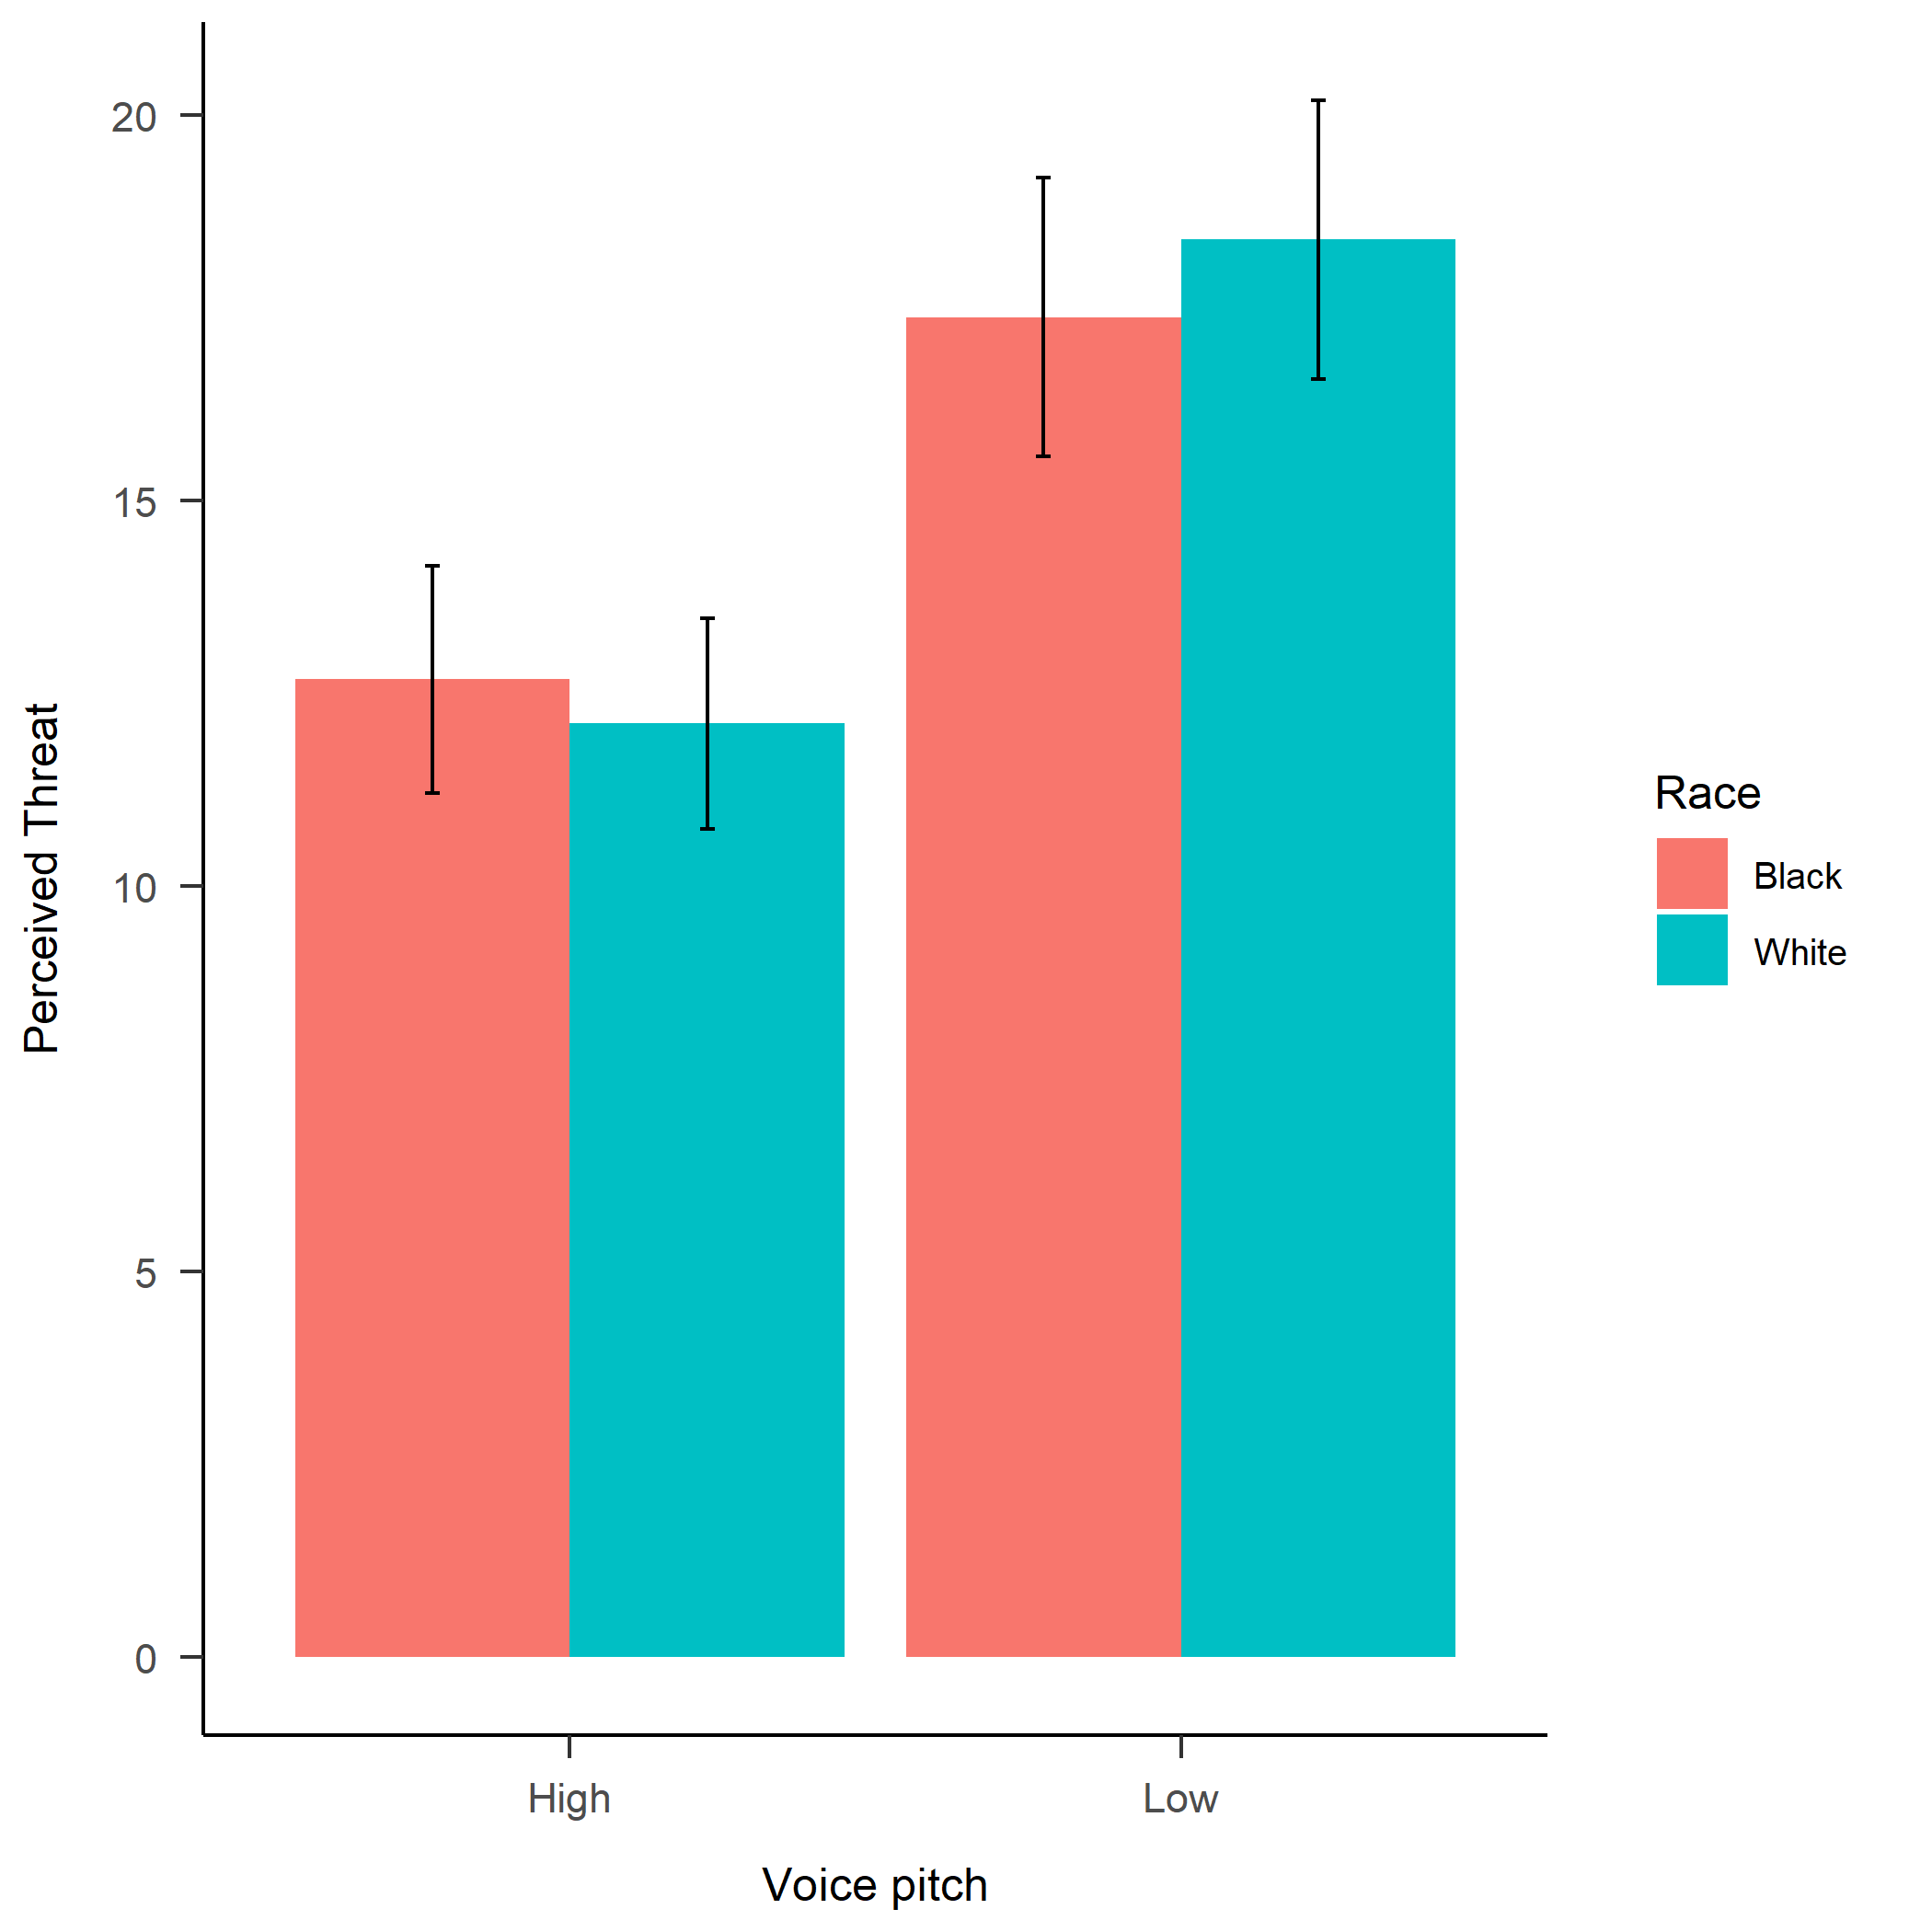
\includegraphics[width=300px]{C:/Users/keana/OneDrive - PennO365/Comp_transfer2018/Penn/stats_masters/stats-masters/figs/fixed_plot1} 

}

\caption{Mean perceptions of threat as a function of voice pitch and perceived race. Error bars represent 95 percent confidence intervals. The perceptions of threat items were on 100 point scales.}\label{fig:f1}
\end{figure}

\hypertarget{effects-of-voice-pitch-and-race-on-perceived-leadership-ability}{%
\subsection{Effects of voice pitch and race on perceived leadership ability}\label{effects-of-voice-pitch-and-race-on-perceived-leadership-ability}}

To determine the effect of voice and race upon perceived leadership ability, we ran a 2 (voice pitch: high or low) X 2 (race: Black or White) analysis with the leadership composite score as the dependent measure. The model specification was as follows: leadership \textasciitilde{} cond\_pitchC + cond\_raceC + cond\_pitchC~\(\times\) cond\_raceC + (1 + cond\_pitchC \textbar{} voice) + (1 \textbar{} id) (Model 2 in Appendix). In contrast to previous studies, voice pitch did not significantly predict perceptions of leadership ability, \(\beta\) = -2.82, \emph{t} = -2.06, \emph{p} = .083. However race significantly predicted perceptions of leadership composite ratings, \(\beta\) = -2.58, \emph{t} = -3.60, \emph{p} \textless{} .001 (see Figure \ref{fig:f2}). Unexpectedly, Black voices were rated higher on leadership traits compared to White voices. The interaction between race and voice pitch on perceived leadership ability was not significant, \(\beta\) = -1.64, \emph{t} = -1.32, \emph{p} = .186.

\begin{figure}

{\centering 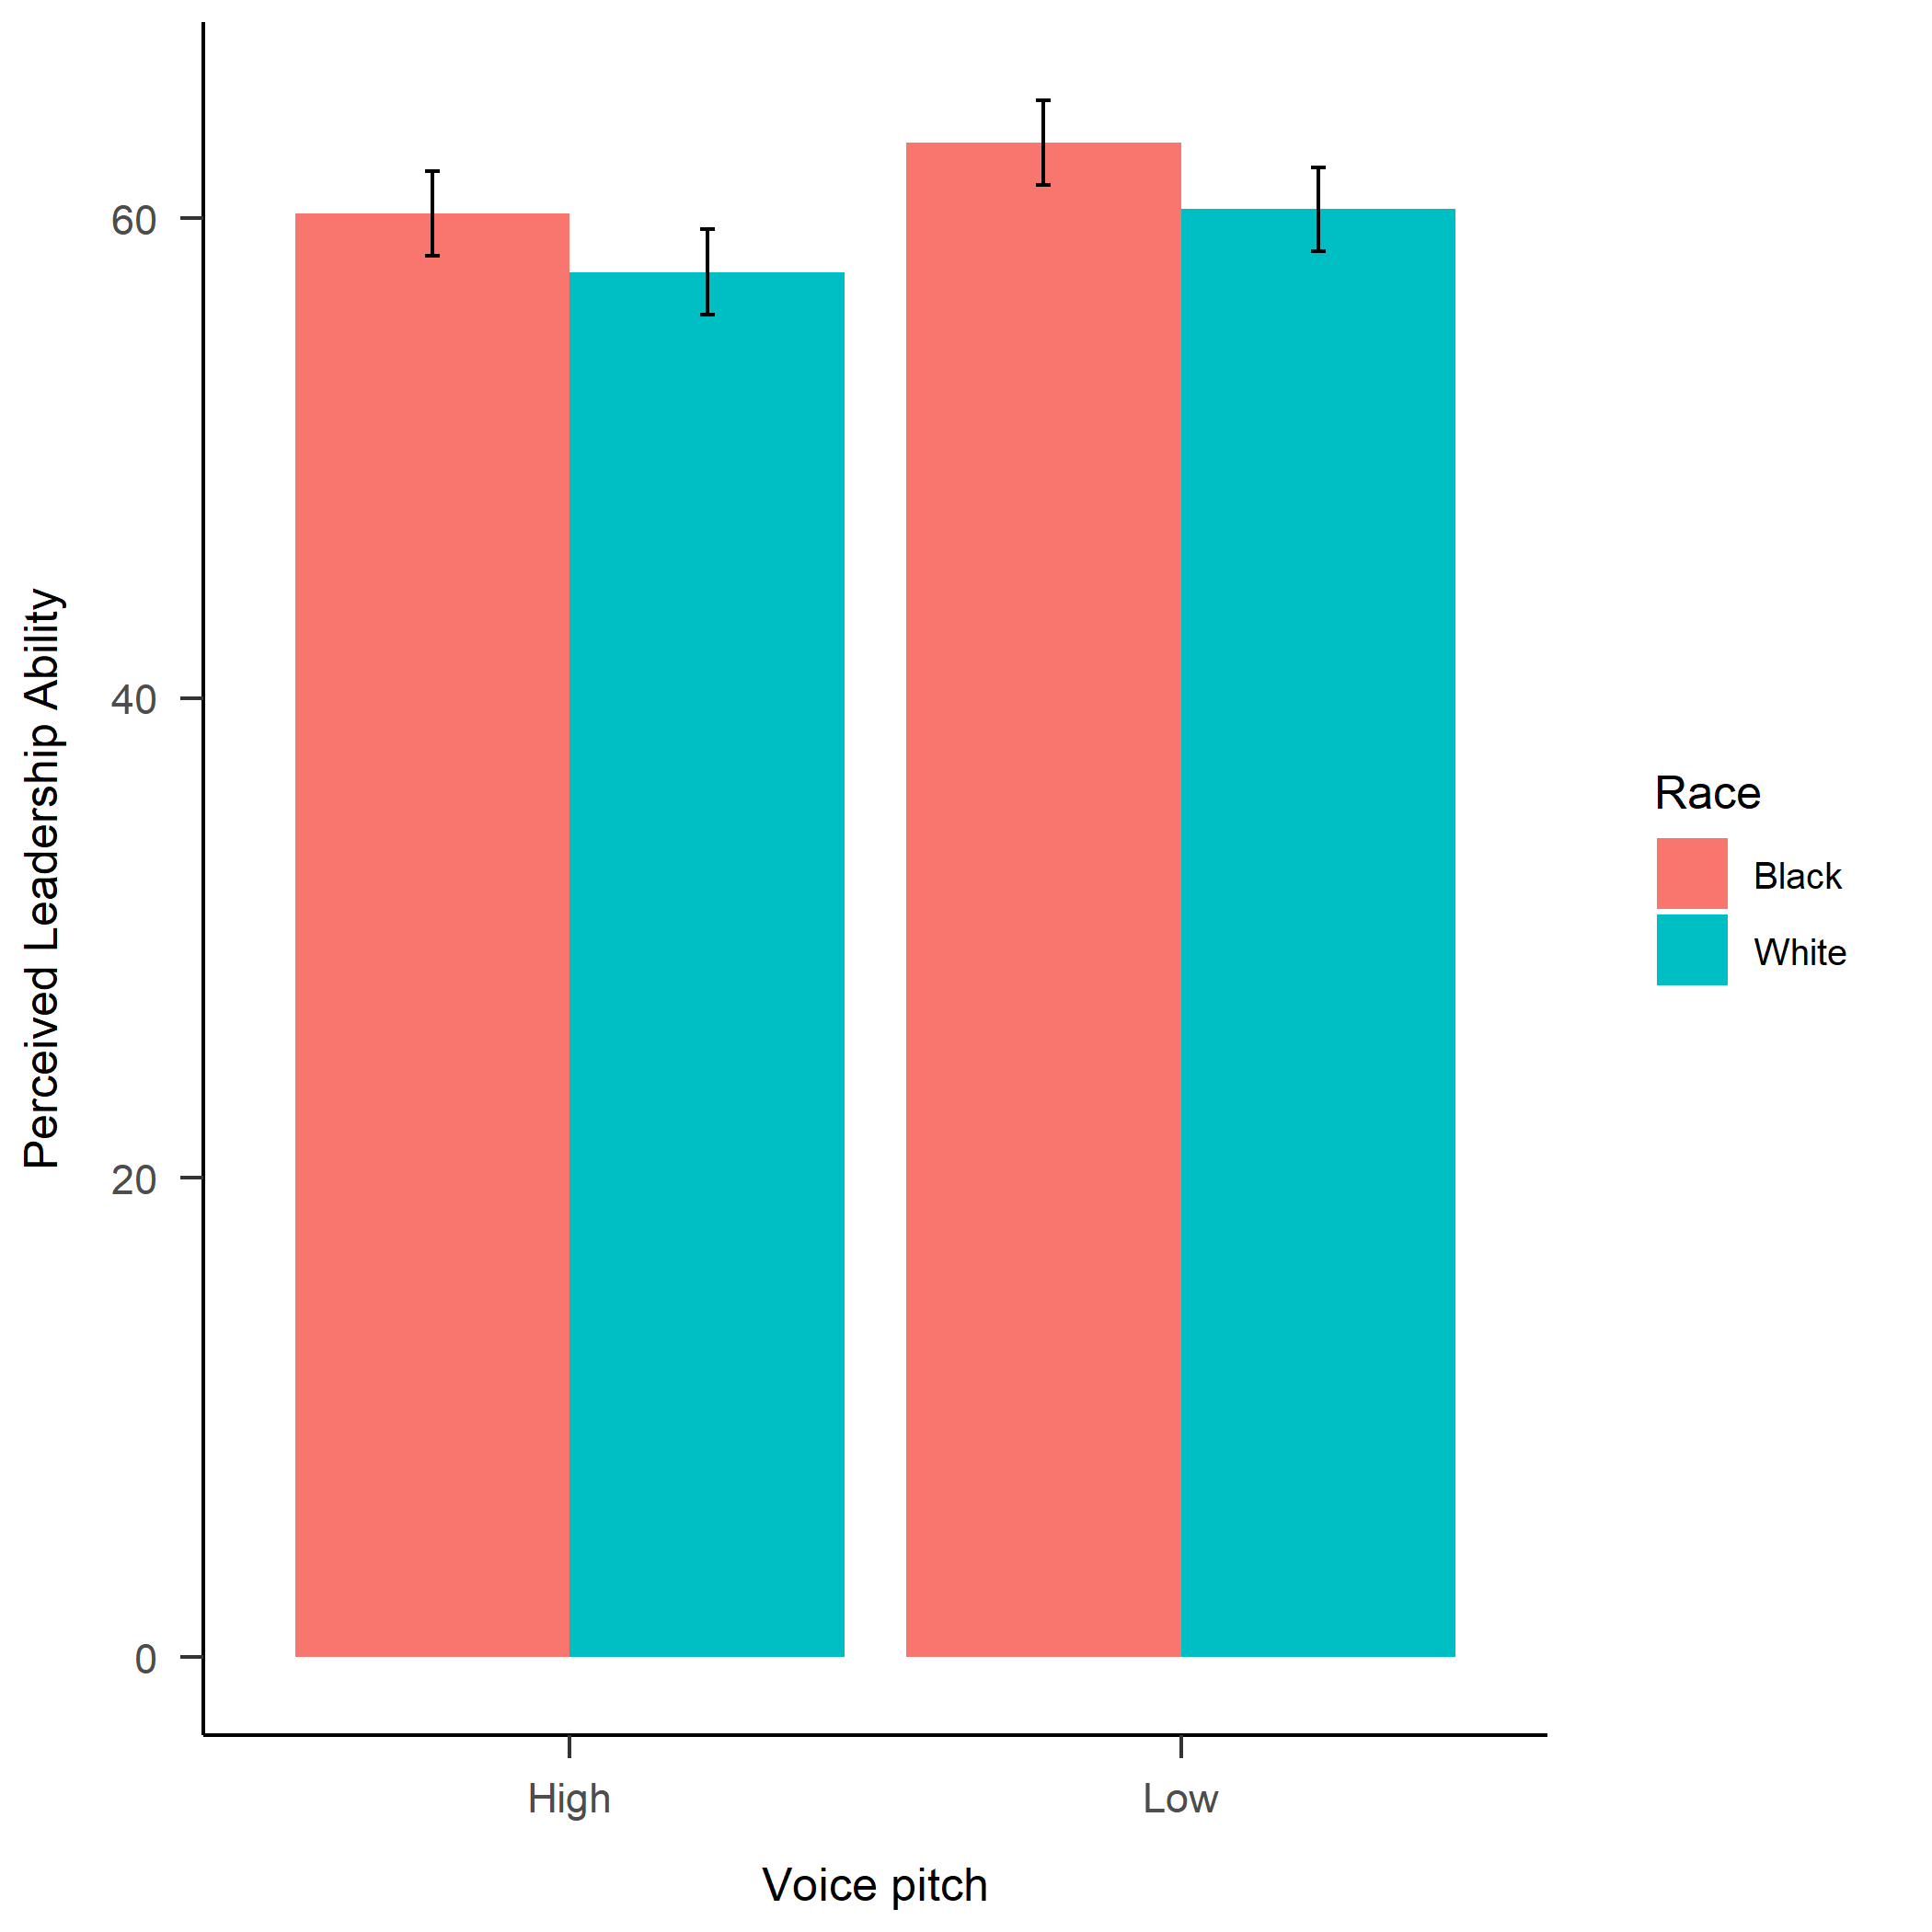
\includegraphics[width=300px]{C:/Users/keana/OneDrive - PennO365/Comp_transfer2018/Penn/stats_masters/stats-masters/figs/fixed_plot2} 

}

\caption{Mean perceptions of leadership traits as a function of voice pitch and perceived race. Error bars represent 95 percent confidence intervals. The perceptions of leadership items were on 100 point scales.}\label{fig:f2}
\end{figure}

\hypertarget{trustworthiness-and-dominance-predicting-threat}{%
\subsection{Trustworthiness and dominance predicting threat}\label{trustworthiness-and-dominance-predicting-threat}}

To examine the relationship between trustworthiness and dominance with perceived threat, we ran a multilevel model with fixed effects for trustworthiness and dominance predicting perceived threat, along with random intercepts for participant and voice. Notably, the Hausman test comparing the fixed effects estimator and random effects estimator for this model suggested that the random effects assumption was not met. Therefore, we employ a CRE model by including the cluster-means for both voice pitch and participant as controls for each fixed effect. The final model specification was as follows: threat \textasciitilde{} trust + dom + trustC\_id + domC\_id +trustC\_voice + domC\_voice + (1 \textbar{} id) + (1 \textbar{} voice) (Model 3 in Appendix). Overall, we found that trustworthiness was negatively related to threat, \(\beta\) = -0.53, \emph{t} = -4.89, \emph{p} = .002, while dominance was positively related to threat, \(\beta\) = 0.45, \emph{t} = 6.40, \emph{p} \textless{} .001.

\hypertarget{effects-of-race-on-perceived-trustworthiness-voice-pitch-on-perceived-dominance}{%
\subsection{Effects of race on perceived trustworthiness \& voice pitch on perceived dominance}\label{effects-of-race-on-perceived-trustworthiness-voice-pitch-on-perceived-dominance}}

To determine the main effect of race upon perceived trustworthiness, we ran a multilevel model with fixed effects for race, perceived trustworthiness as the dependent measure, and random effects for participant and voice to examine whether race altered perceptions of trustworthiness. Based on our random effects selection criteria, we ran the following model: trust \textasciitilde{} cond\_raceC + (1 \textbar{} id) + (1 \textbar{} voice) (Model 4 in Appendix). There was a marginally significant effect of race upon perceived trustworthiness, \(\beta\) = -1.46, \emph{t} = -1.97, \emph{p} = .049, where Black men were perceived as more trustworthy than White men.

We also tested whether voice pitch predicted perceived dominance with perceived dominance as the dependent measure using the following random effects specification: dom \textasciitilde{} cond\_pitchC + (1 \textbar{} voice) + (1 \textbar{} id) (Model 5 in Appendix). The effect of voice pitch on perceived dominance was significant, \(\beta\) = -8.80, \emph{t} = -9.59, \emph{p} \textless{} .001, where higher-pitched voices were less likely to be perceived as dominant.

\hypertarget{interaction-between-voice-pitch-and-race-on-perceived-threat-potential}{%
\subsection{Interaction between voice pitch and race on perceived threat potential}\label{interaction-between-voice-pitch-and-race-on-perceived-threat-potential}}

For our last pre-registered analysis, we examined the effect of voice pitch and race on perceived threat potential, a composite score created by averaging ratings of dominance and reverse-scored ratings of trust (by subtracting each rating from 100) within each condition. For instance, if a participant perceives a voice as extremely dominant (e.g., rating of 95), but also high in trustworthiness (e.g., rating of 95 on original trust measure, -95 after reverse-scoring), their overall threat potential score will be 0. On the other hand, participants rated low on trustworthiness and high on dominance will have high threat potential ratings. This analysis serves as a means of conceptually replicating the primary analysis with voice pitch and race predicting ratings of perceived threat. As suggested previously, research suggests that faces perceived as dominant and untrustworthy are the most likely to be perceived as threatening (Oosterhof \& Todorov, 2008). We expect voices will be categorized in a similar manner, and as such, our findings from the primary analysis with voice pitch and race predicting perceived threat will be replicated using the perceived threat potential composite measure as a proxy for perceived threat. The perceived threat potential measure was submitted as the dependent variable to a multilevel model with the following random effects structure: threatpotential \textasciitilde{} cond\_raceC + cond\_pitchC + cond\_raceC~\(\times\) cond\_pitchC + (1 + cond\_pitchC \textbar{} voice) + (1 \textbar{} id) (Model 6 in Appendix). We find evidence that voice pitch significantly predicts perceived threat potential, \(\beta\) = -5.36, \emph{t} = -5.31, \emph{p} = .002, with higher pitched voices perceived as less threatening. However, we do not find evidence of a significant effect of race, , \(\beta\) = -0.04, \emph{t} = -0.08, \emph{p} = .936, nor the interaction between race and voice pitch, \(\beta\) = -1.05, \emph{t} = -1.01, \emph{p} = .314.

\hypertarget{discussion}{%
\section{Discussion}\label{discussion}}

Overall, we found that voice pitch has a significant effect upon perceived threat, where lower-pitched voices were rated as more threatening compared to their higher-pitched counterparts, replicating previous literature on this topic (Hodges-Simeon et al., 2014). Our original primary hypotheses were not supported, since we did not find the expected interaction effects of voice pitch and race on perceived threat or perceived leadership. Instead, we found an unexpected effect of race upon leadership, where Black men were rated significantly higher on perceived leadership compared to White men. This finding contradicted our expectations, since most other research on this topic suggests that White men are prototypical leaders and are much more likely to be rated higher on perceived leadership than other social groups (Rosette et al., 2008). With regards to our secondary hypotheses, we find support for our prediction that perceived trustworthiness and perceived dominance would be related to perceived threat in the expected directions. Specifically, perceived trustworthiness was negatively related to perceived threat and perceived dominance was positively related to perceived threat across all conditions. This aligns with previous research examining the effect of facial dominance and trustworthiness on person perception, which shows that these characteristics are combined to affect perceived threat (Oosterhof \& Todorov, 2008), but no studies have examined this relationship based upon vocal characteristics and race before. Therefore, our study provides preliminary support for the notion that the observed effects of facial trustworthiness and dominance on threat can be generalized to other personal characteristics (i.e., the voice).

Regarding our other secondary hypotheses, we found a significant effect of race upon perceived trustworthiness, but in the opposite direction of our expectations, where Black men were rated as significantly more trustworthy compared to White men. Most of the literature in this domain suggests that Black men are perceived as less trustworthy (Stanley, Sokol-Hessner, Banaji, \& Phelps, 2011; Stanley et al., 2012), largely because of negative stereotypes that are applied to their social category. Additionally, we found the expected effect of voice pitch on perceived dominance.

In future research, we intend to address several limitations in our methodology that may have affected our results. Specifically, we only used White male voices, most of whom were graduate students at the University of Pennsylvania, which allowed us to have a relatively homogeneous sample of stimuli. Although race cannot be detected from the voice, SES and education levels are reflected by vocal characteristics, so it is entirely possible that participants were expecting the voices associated with stereotypically Black names (which tend to be associated with low SES) to speak with African American Vernacular English (Labov, 2010). However, many of the voices we used as stimuli were from individuals that were attaining a much higher standard of education (PhD students) compared to the average individual, which may be obvious in their speech patterns. Additionally, the threat item was not situated in any context (i.e., participants were not provided any background as to why the voices should be perceived as threatening), and it is possible that participants interpreted the question of threateningness in different ways (i.e., physical threat, threat to resources, etc.). We observed the expected effect of voice pitch upon perceived threat and threat potential, which may reflect an innate understanding of how sounds can convey threat, which is observed even in infancy (e.g., larger objects produce a lower pitch) (Vestergaard et al., 2009). On the other hand, race is not an evolutionarily-relevant coalitional cue, but instead is constructed as a cue of coalitional alliances through ecological conditions (Kurzban \& Leary, 2001), so it is unlikely that the manipulation of race elicited the perceptions of threat to the same degree as the voice manipulations. Since the study was conducted online and approximately half of the participants indicated that they listened to the recordings through speakers, it is also possible that there may have been differences in the listening environment that prevented participants from picking up on the differences in our voice pitch manipulations. Finally, we did not ask participants whether they thought the study was real, which may have provided more information about our observed results, since it is entirely possible that participants answered the suspicion check to align with the cover story because they thought it might have been an attention check.

It is imperative that future research within this domain attempts to address some of these limitations and determine whether the results are generalizable and replicable. Future studies should recruit a more diverse sample for vocal stimuli, including women and people from different racial groups and education levels. It would be useful to ask participants to guess which race and education level each voice represents to determine whether these characteristics will moderate the relationship between the independent variables and perceived leadership. Other studies (Hester \& Gray, 2018) have included endorsement of stereotypes as a moderator for explaining higher ratings on stereotype-consistent items, which would be valuable in future extensions of this research. Finally, reversing the playback of the recordings may allow us to reduce the effects of speech content and vernacular upon participants' ratings.

It will also be important to disentangle the possible explanations for our unexpected effect of race upon perceived leadership. There are a few possible explanations for these results, which we will discuss briefly, along with ways to address these possible explanations in future research. First, social demand effects are always a concern when running within-subjects studies about race, because people are averse to being considered biased against Black people. When participants were presented 2 White names and 2 Black names (in a random order), it is entirely possible that they guessed that the study was focused on perceptions based upon race. Although we included a suspicion check and excluded participants based upon stringent criteria, the suspicion check may have biased participants to indicate that they were not suspicious. Specifically, they had to type in a text entry box if they were suspicious about the hypotheses, whereas they could simply select a multiple-choice option to indicate that they were not aware of the hypotheses. As a result, participants may have chosen the easier multiple-choice option on the suspicion check instead of choosing to type in their actual prediction of the purpose of the study. Future research can overcome social demand effects by offering to pay participants to tell the truth.

Another potential explanation for our unexpected results is contrast effects, which are based upon the shifting stereotypes model (Biernat, Manis, \& Nelson, 1991). This model posits that an individual will judge others on stereotype-relevant dimensions relative to other individuals within their social category. In the case of our study, the order of presentation of the name and voice stimuli may have affected the outcomes, since the stereotypical Black names were presented before the voices. This may have preempted them to expect a voice that sounded relatively uneducated. Previous research shows that the voice can convey SES and education levels (Kreiman \& Sidtis, 2011), so it is entirely possible that participants used this information in their assessments of the individuals in the recordings. Since the individuals that we recruited for our voice stimuli were generally well-educated (University of Pennsylvania graduate students and upper-level undergraduates) relative to the general population, the Black voices might have exceeded their low expectations, eliciting higher ratings. On the contrary, White men tend to have positive stereotypes attributed to them regarding their leadership ability (Rosette et al., 2008), so the baseline expectations for the White voices were relatively high, which may have also contributed to the effect of race upon perceived leadership ability. Future studies should use more objective measures of leadership, since contrast effects are more likely to appear when participants are rating stimuli on subjective measures (e.g., Likert-type items) because these ratings may vary across contexts, while objective measures are consistent, regardless of the target, the perceiver, or immediate environmental influences (Biernat, 2003). If future studies replicate the current study design but replace the leadership composite with objective measures and do not find a similar effect of race upon leadership, this will provide support for contrast effects upon our results.

The final explanation that we encourage future researchers to explore is the possibility that Black men were rated higher on leadership because, in the absence of threat, they may benefit from stereotypes that typically attribute dominance and aggressiveness to their social group (Devine \& Elliot, 1995). Dominance and aggressiveness were invaluable characteristics for leaders throughout our evolutionary history who needed to be successful during lethal inter-group conflicts and dangerous hunting sessions (Van Vugt, Johnson, Kaiser, \& O'Gorman, 2008). Therefore, any personal characteristics that are perceived as more dominant or aggressive may increase perceived leadership ability, even though these traits may not accurately reflect leadership ability in the modern day (Klofstad \& Anderson, 2018; Li, Vugt, \& Colarelli, 2017). In this way, Black men might have been rated as better leaders because they were attributed dominance and aggressiveness to a greater degree than White men based upon stereotypes.

Future extensions of this research will be fruitful in helping us fully understand the complex interplay of vocal characteristics and racial stereotypes in affecting person perception. As other research has demonstrated, Black men are more likely to be perceived as threatening (Trawalter, Todd, Baird, \& Richeson, 2008; Wilson et al., 2017), which can be detrimental to their success in leadership positions when they are typically the minority in the corporate world. There is preliminary evidence in support of the concept that Black men that have disarming mechanisms may benefit from these personal characteristics in leadership positions (Hester \& Gray, 2018; Livingston \& Pearce, 2009; Wilson et al., 2017). Although the current study did not find the expected interaction effects of voice pitch and race upon perceived threat and leadership, there is still room for improvement in the methodological design and we encourage future researchers to extend this line of work to explore possible explanations further.

This line of work is important in helping us disentangle the personal characteristics that have a major effect upon person perception. Since we are incapable of reading others' minds to assess their intentions, we usually must make judgments of their character based upon their personal characteristics, even if these traits may not always be linked to their trustworthiness and/or threat potential. In this way, stereotypes about their group (based upon their observable characteristics that cue group membership) and their personal characteristics that cue their ability to act upon any threatening intentions combine to predict trust towards that person.

The stereotype that Black people are a threat to physical safety and personal property has permeated largely because race and ecology are confounded in the United States, such that Black people are more likely to be impoverished, which is intricately linked with crime risk (Williams, Yu, Jackson, \& Anderson, 1997; Williams, Sng, \& Neuberg, 2016). Along these lines, Black people are overrepresented in certain contexts that link them with threat to physical safety (e.g., prisons) (Mauer \& King, 2007; Roberts, 2004). Over time, Americans began to associate crime with any individuals categorized as Black (Quillian \& Pager, 2001). These stereotypes are especially likely to be spread in the modern context, since there are a multitude of technologies available for communicating with numerous individuals regardless of interpersonal distance, which encourages the uniform and rapid spread of information across a culture. Also, popular press facilitates this stereotyping by reporting racialized crime stories that strengthen the association between race and physical threat (Dixon \& Azocar, 2007; Gilliam, Iyengar, Simon, \& Wright, 1996). Through these mechanisms, stereotypes have become ingrained in the public conscious in America today, and continue to affect how Black people are treated daily, even after explicit prejudice has become less socially acceptable (Murphy, Richeson, Shelton, Rheinschmidt, \& Bergsieker, 2013). Since many of the stereotypes in America are rooted in protracted racial tensions throughout history, any intervention to reduce these stereotypes must be comprehensive, targeting the many factors that contribute to stereotypes about Black people. Specifically, it is possible that the voice may serve as a potent disarming mechanism that can reduce perceived threat in Black men, which we explored through the current study. This research provides an initial glimpse into how certain vocal characteristics can be affected by racial stereotypes, but future research needs to continue this line of work to enlighten us about the importance of nonverbal behavior in influencing perceptions of, and in turn, behavior towards minority individuals.

\hypertarget{appendix}{%
\section{Appendix}\label{appendix}}

\hypertarget{perceptions-of-race-based-on-name}{%
\subsection{Perceptions of race based on name}\label{perceptions-of-race-based-on-name}}

\begin{figure}

{\centering 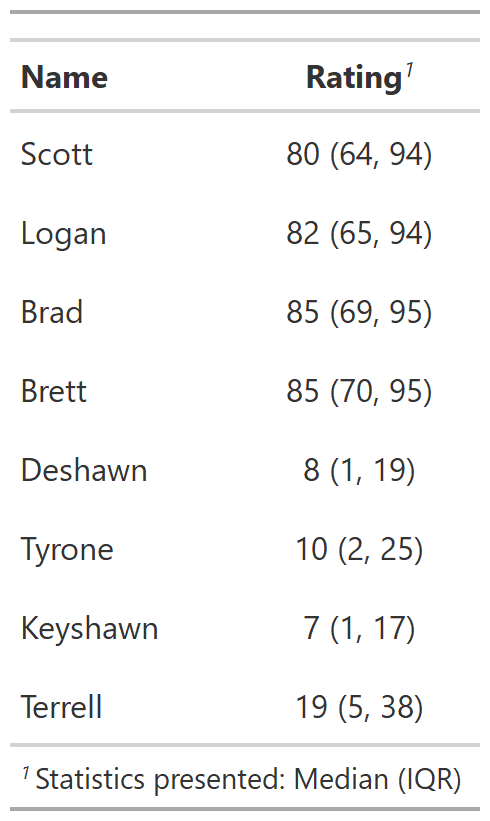
\includegraphics[width=0.35\linewidth]{C:/Users/keana/OneDrive - PennO365/Comp_transfer2018/Penn/stats_masters/stats-masters/figs/MC_ratingsw_tbl} 

}

\caption{Participants' responses to the question "Based upon the names below, please rate the likelihood that the person is White:" on 100 point slider scale.}\label{fig:f3}
\end{figure}

\begin{figure}

{\centering 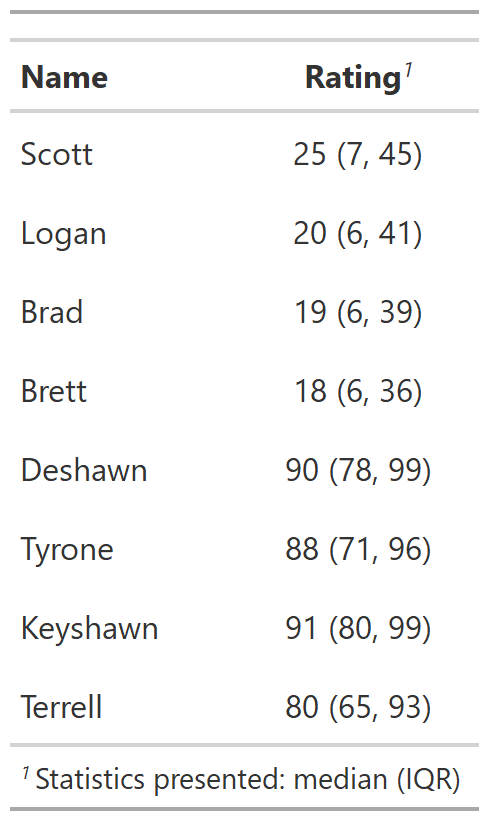
\includegraphics[width=0.35\linewidth]{C:/Users/keana/OneDrive - PennO365/Comp_transfer2018/Penn/stats_masters/stats-masters/figs/MC_ratingsb_tbl} 

}

\caption{Participants' responses to the question "Based upon the names below, please rate the likelihood that the person is Black:" on 100 point slider scale.}\label{fig:f4}
\end{figure}

\hypertarget{final-models}{%
\subsection{Final models}\label{final-models}}

\begin{figure}

{\centering 
\includegraphics[width=0.85\linewidth]{C:/Users/keana/OneDrive - PennO365/Comp_transfer2018/Penn/stats_masters/stats-masters/figs/final_table1} 

}

\caption{Summary of Model 1: Effects of voice pitch and race on perceived threat. The dependent variable is participants' ratings of threat, from 0 to 100. See the methods subsection titled "Multilevel modeling methodology for current research" for a summary of the random effects section interpretation. p < .05 are bolded.}\label{fig:f5}
\end{figure}

\begin{figure}

{\centering 
\includegraphics[width=0.85\linewidth]{C:/Users/keana/OneDrive - PennO365/Comp_transfer2018/Penn/stats_masters/stats-masters/figs/final_table2} 

}

\caption{Summary of Model 2: Effects of voice pitch and race on perceived leadership ability. The dependent variable is the composite measure of leadership ability, which was created by averaging participants' ratings of intelligence, effective communication, confidence, and problem-solving ability (all from 0 to 100). See the methods subsection titled "Multilevel modeling methodology for current research" for a summary of the random effects section interpretation. p < .05 are bolded.}\label{fig:f6}
\end{figure}

\begin{figure}

{\centering 
\includegraphics[width=0.85\linewidth]{C:/Users/keana/OneDrive - PennO365/Comp_transfer2018/Penn/stats_masters/stats-masters/figs/final_table3} 

}

\caption{Summary of Model 3: Trustworthiness and dominance predicting perceived threat. The dependent variable is participants' ratings of threat, from 0 to 100. See the methods subsection titled "Multilevel modeling methodology for current research" for a summary of the random effects section interpretation. p < .05 are bolded.}\label{fig:f7}
\end{figure}

\begin{figure}

{\centering 
\includegraphics[width=0.85\linewidth]{C:/Users/keana/OneDrive - PennO365/Comp_transfer2018/Penn/stats_masters/stats-masters/figs/final_table5} 

}

\caption{Summary of Model 4: Effects of race on perceived trustworthiness. The dependent variable is participants' ratings of trustworthiness, from 0 to 100. See the methods subsection titled "Multilevel modeling methodology for current research" for a summary of the random effects section interpretation. p < .05 are bolded.}\label{fig:f8}
\end{figure}

\begin{figure}

{\centering 
\includegraphics[width=0.85\linewidth]{C:/Users/keana/OneDrive - PennO365/Comp_transfer2018/Penn/stats_masters/stats-masters/figs/final_table6} 

}

\caption{Summary of Model 5: Effects of voice pitch on perceived dominance. The dependent variable is participants' ratings of dominance, from 0 to 100. See the methods subsection titled "Multilevel modeling methodology for current research" for a summary of the random effects section interpretation. p < .05 are bolded.}\label{fig:f9}
\end{figure}

\begin{figure}

{\centering 
\includegraphics[width=0.85\linewidth]{C:/Users/keana/OneDrive - PennO365/Comp_transfer2018/Penn/stats_masters/stats-masters/figs/final_table7} 

}

\caption{Summary of Model 6: Effects of voice pitch and race on perceived threat potential. The dependent variable is threat potential, a composite measure averaging participants' ratings of dominance and reverse-scored trustworthiness (both on 100 point scales). See the methods subsection titled "Multilevel modeling methodology for current research" for a summary of the random effects section interpretation. p < .05 are bolded.}\label{fig:f10}
\end{figure}

\hypertarget{model-comparison}{%
\subsection{Model comparison}\label{model-comparison}}

\begin{figure}

{\centering 
\includegraphics[width=0.85\linewidth]{C:/Users/keana/OneDrive - PennO365/Comp_transfer2018/Penn/stats_masters/stats-masters/figs/compare_table1} 

}

\caption{Comparing maximal, final, and robust versions of Model 1: Effects of voice pitch and race on perceived threat. The dependent variable across models is participants' ratings of threat, from 0 to 100. See the methods subsection titled "Multilevel modeling methodology for current research" for a summary of the random effects section interpretation. p < .05 are bolded.}\label{fig:f11}
\end{figure}

\begin{figure}

{\centering 
\includegraphics[width=0.85\linewidth]{C:/Users/keana/OneDrive - PennO365/Comp_transfer2018/Penn/stats_masters/stats-masters/figs/compare_table2} 

}

\caption{Comparing maximal, final, and robust versions of Model 2: Effects of voice pitch and race on perceived leadership ability. The dependent variable across models is the composite measure of leadership ability, which was created by averaging participants' ratings of intelligence, effective communication, confidence, and problem-solving ability (all from 0 to 100). See the methods subsection titled "Multilevel modeling methodology for current research" for a summary of the random effects section interpretation. p < .05 are bolded.}\label{fig:f12}
\end{figure}

\begin{figure}

{\centering 
\includegraphics[width=0.85\linewidth]{C:/Users/keana/OneDrive - PennO365/Comp_transfer2018/Penn/stats_masters/stats-masters/figs/compare_table3} 

}

\caption{Comparing maximal, final, and robust versions of Model 3: Trustworthiness and dominance predicting threat. The dependent variable across models is participants' ratings of threat, from 0 to 100. See the methods subsection titled "Multilevel modeling methodology for current research" for a summary of the random effects section interpretation. p < .05 are bolded.}\label{fig:f13}
\end{figure}

\begin{figure}

{\centering 
\includegraphics[width=0.85\linewidth]{C:/Users/keana/OneDrive - PennO365/Comp_transfer2018/Penn/stats_masters/stats-masters/figs/compare_table5} 

}

\caption{Comparing maximal, final, and robust versions of Model 4: Effects of race on perceived trustworthiness. The dependent variable across models is participants' ratings of trustworthiness, from 0 to 100. See the methods subsection titled "Multilevel modeling methodology for current research" for a summary of the random effects section interpretation. p < .05 are bolded.}\label{fig:f14}
\end{figure}

\begin{figure}

{\centering 
\includegraphics[width=0.85\linewidth]{C:/Users/keana/OneDrive - PennO365/Comp_transfer2018/Penn/stats_masters/stats-masters/figs/compare_table6} 

}

\caption{Comparing maximal, final, and robust versions of Model 5: Effects of voice pitch on perceived dominance. The dependent variable across models is participants' ratings of dominance, from 0 to 100. See the methods subsection titled "Multilevel modeling methodology for current research" for a summary of the random effects section interpretation. p < .05 are bolded.}\label{fig:f15}
\end{figure}

\begin{figure}

{\centering 
\includegraphics[width=0.85\linewidth]{C:/Users/keana/OneDrive - PennO365/Comp_transfer2018/Penn/stats_masters/stats-masters/figs/compare_table7} 

}

\caption{Comparing maximal, final, and robust versions of Model 6: Effects of voice pitch and race on perceived threat potential. The dependent variable across models is threat potential, a composite measure averaging participants' ratings of dominance and reverse-scored trustworthiness (both on 100 point scales). See the methods subsection titled "Multilevel modeling methodology for current research" for a summary of the random effects section interpretation. p < .05 are bolded.}\label{fig:f16}
\end{figure}

\hypertarget{assumption-checking}{%
\subsection{Assumption checking}\label{assumption-checking}}

\begin{figure}
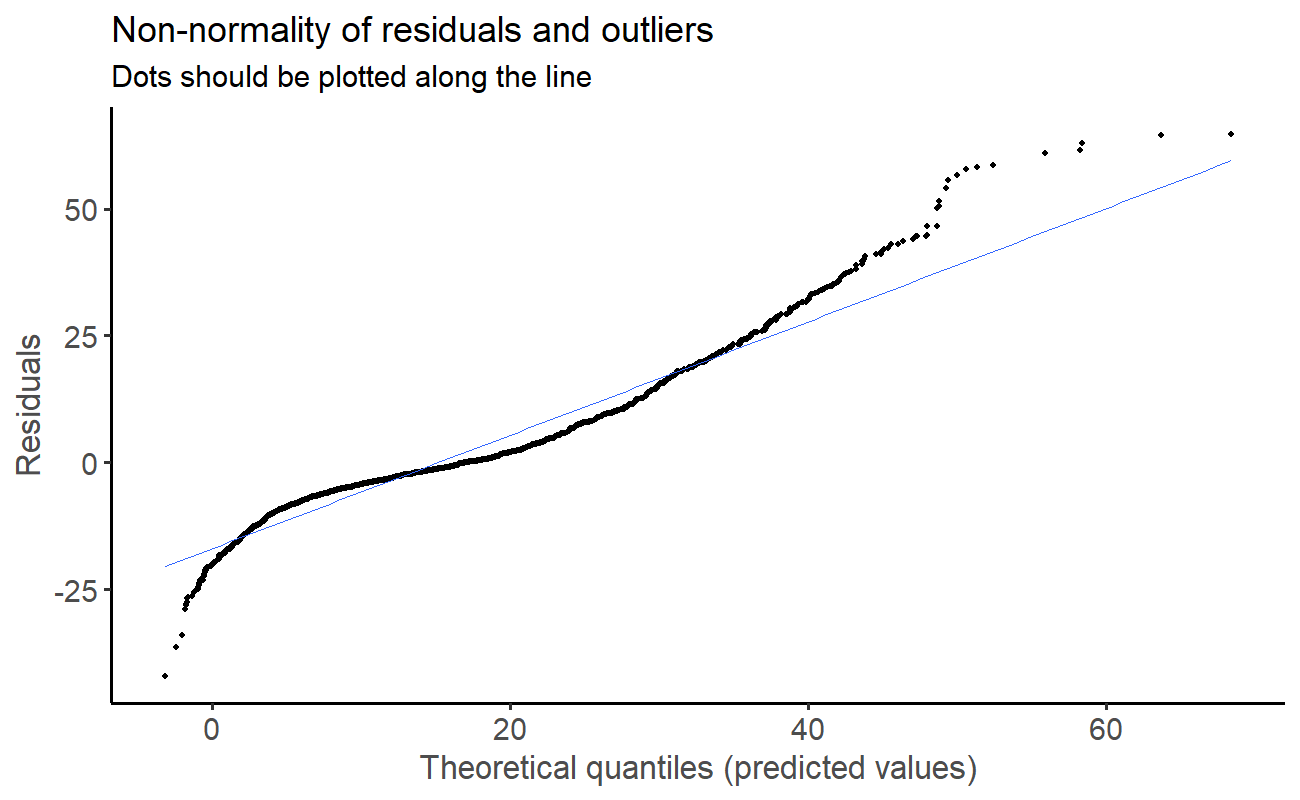
\includegraphics[width=0.5\linewidth]{C:/Users/keana/OneDrive - PennO365/Comp_transfer2018/Penn/stats_masters/stats-masters/figs/asm_mod1.1} 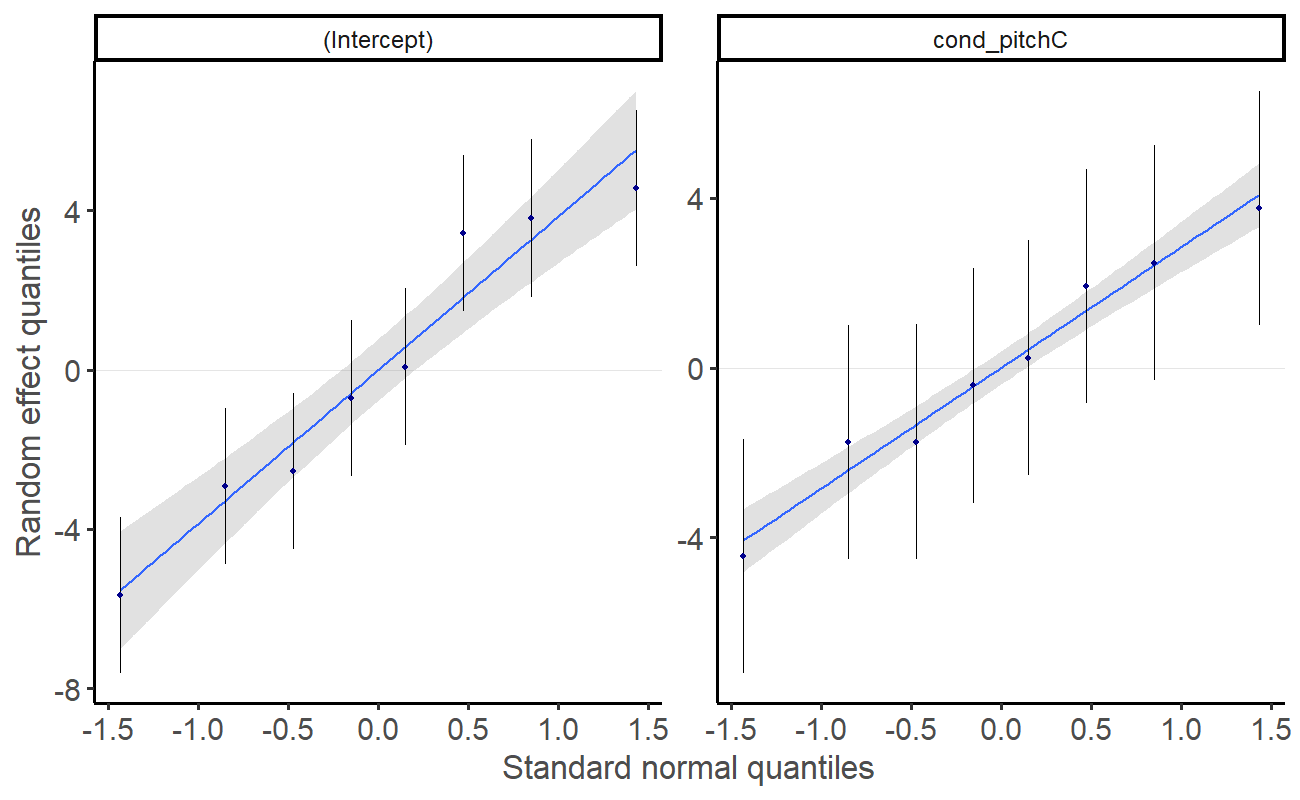
\includegraphics[width=0.5\linewidth]{C:/Users/keana/OneDrive - PennO365/Comp_transfer2018/Penn/stats_masters/stats-masters/figs/asm_mod1.2} 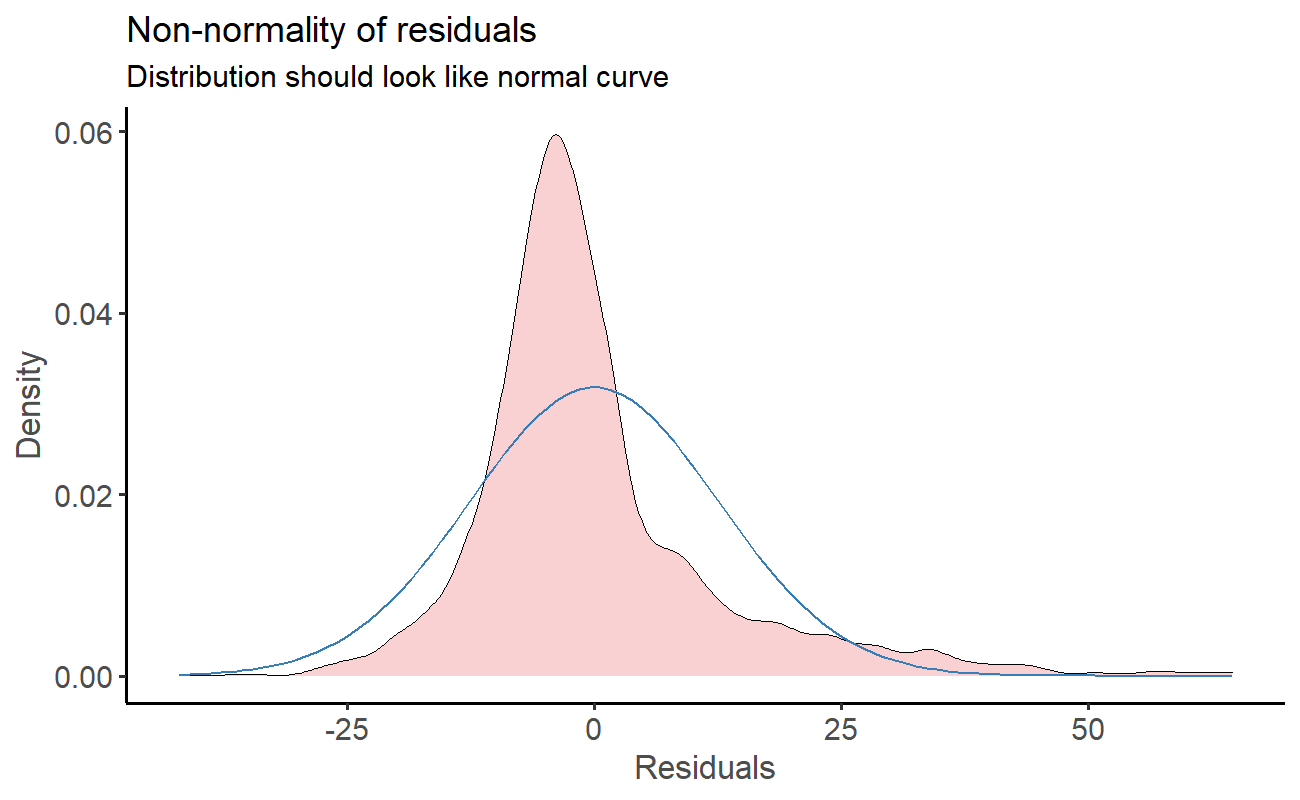
\includegraphics[width=0.5\linewidth]{C:/Users/keana/OneDrive - PennO365/Comp_transfer2018/Penn/stats_masters/stats-masters/figs/asm_mod1.3} 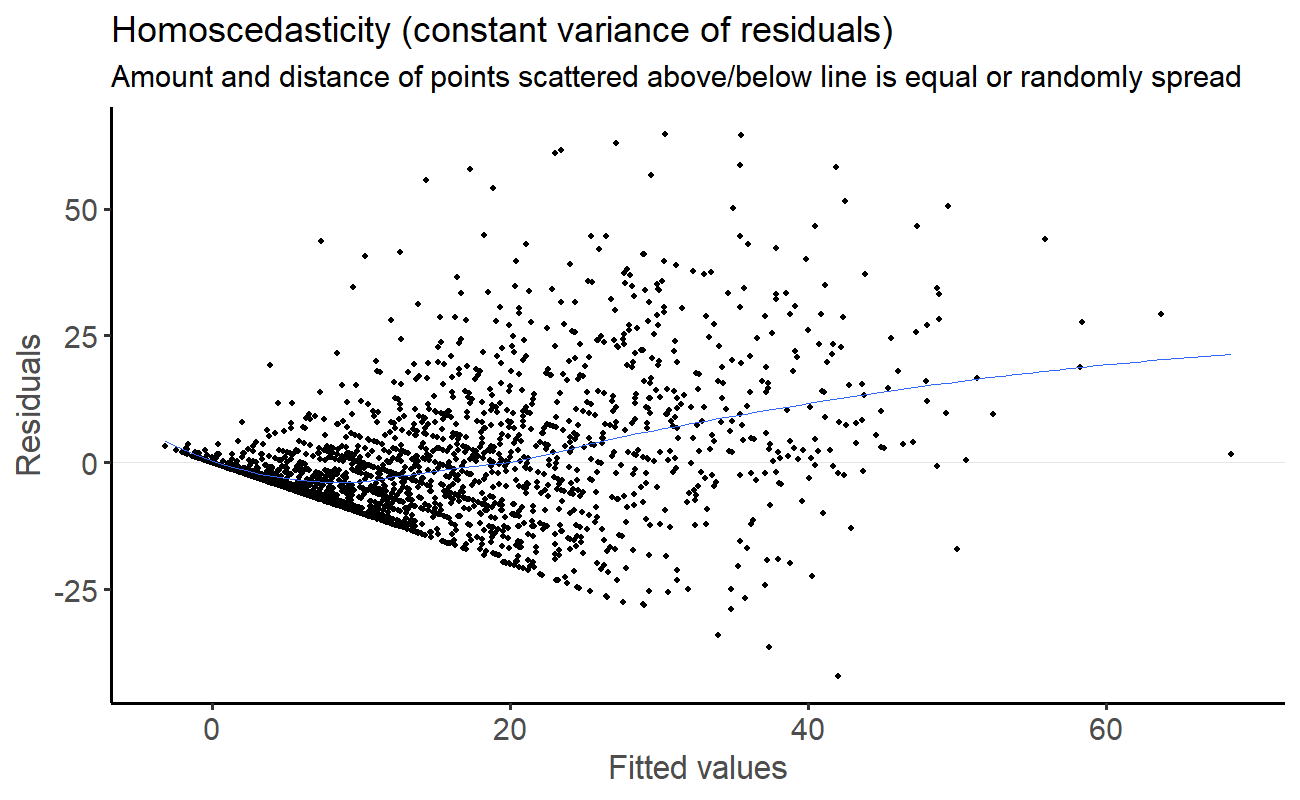
\includegraphics[width=0.5\linewidth]{C:/Users/keana/OneDrive - PennO365/Comp_transfer2018/Penn/stats_masters/stats-masters/figs/asm_mod1.4} \caption{Assumptions for Model 1: Effects of voice pitch and race on perceived threat. Overall, the plots suggest that the assumptions of normality and homoscedasicity may not have been met. For instance, the plot in the lower left-hand corner of the panel shows that the residuals do not appear to follow a normal curve. The plot in the lower right-hand corner shows a pattern, suggesting heteroscedasticity, where the points appear to be cut off sharply in the lower range of the values. Thus, readers are encouraged to compare the effects in the final and robust versions of the model.}\label{fig:f17}
\end{figure}

\begin{figure}
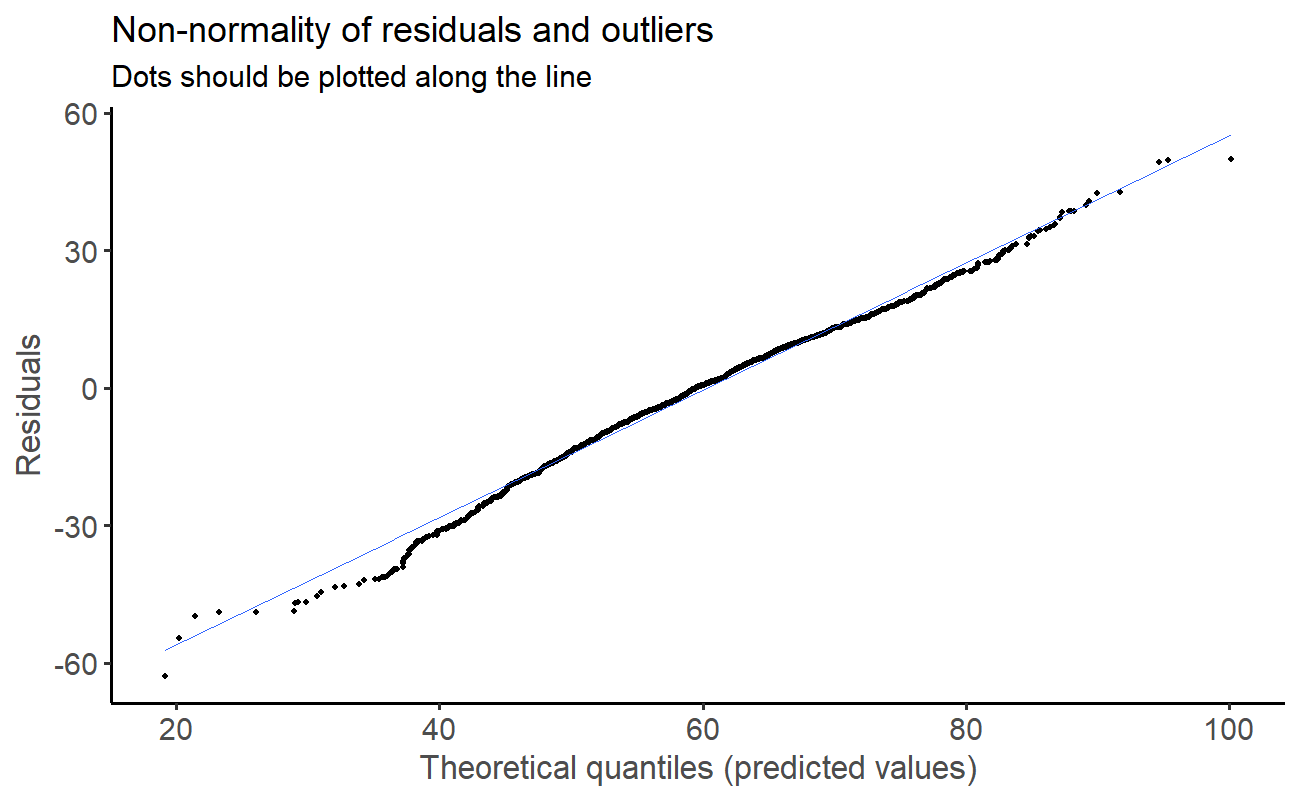
\includegraphics[width=0.5\linewidth]{C:/Users/keana/OneDrive - PennO365/Comp_transfer2018/Penn/stats_masters/stats-masters/figs/asm_mod2.1} 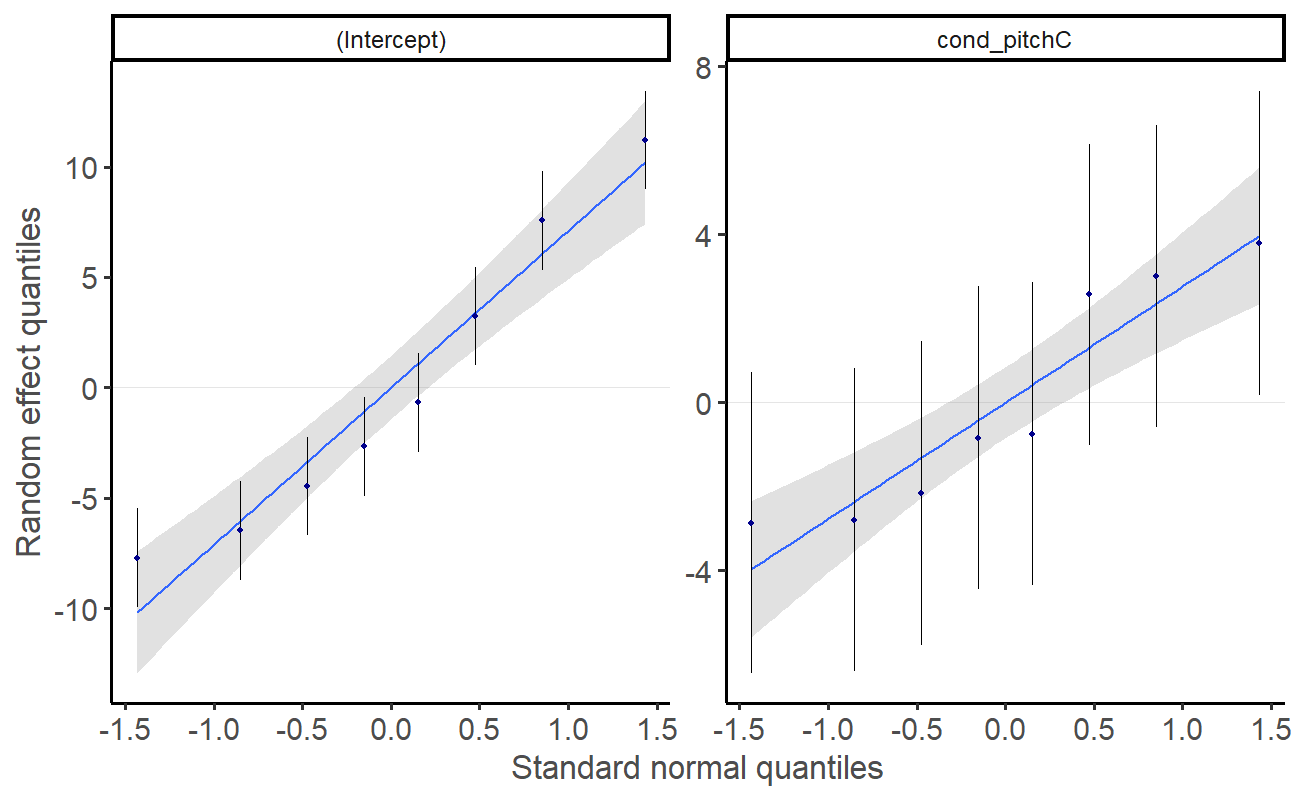
\includegraphics[width=0.5\linewidth]{C:/Users/keana/OneDrive - PennO365/Comp_transfer2018/Penn/stats_masters/stats-masters/figs/asm_mod2.2} 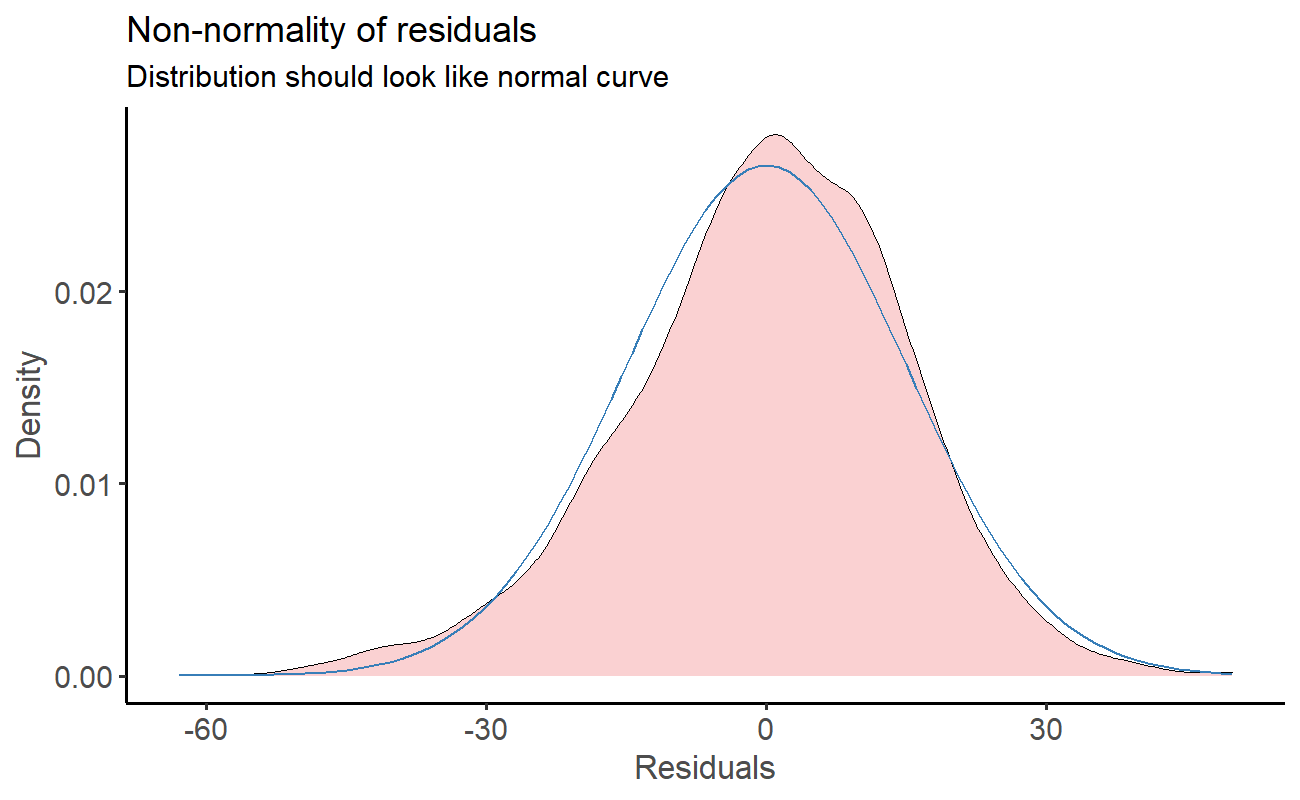
\includegraphics[width=0.5\linewidth]{C:/Users/keana/OneDrive - PennO365/Comp_transfer2018/Penn/stats_masters/stats-masters/figs/asm_mod2.3} 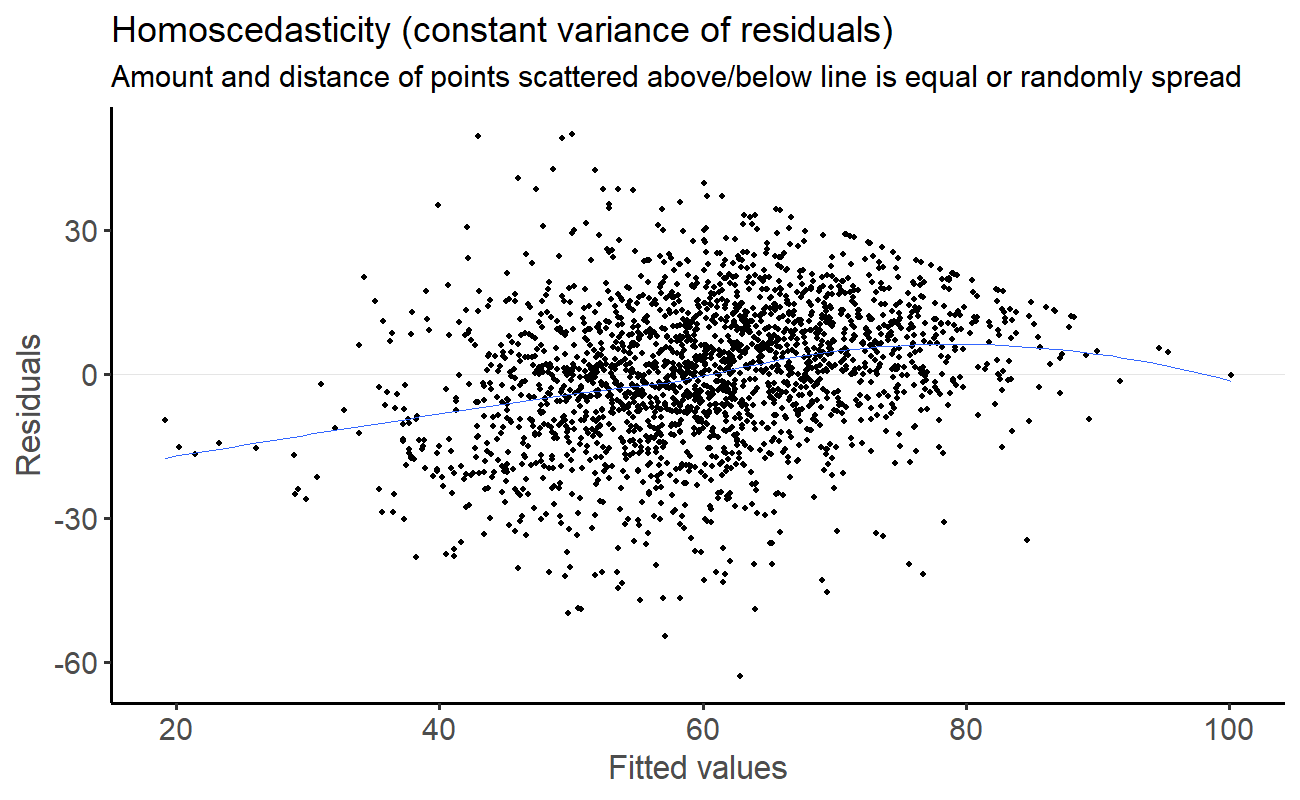
\includegraphics[width=0.5\linewidth]{C:/Users/keana/OneDrive - PennO365/Comp_transfer2018/Penn/stats_masters/stats-masters/figs/asm_mod2.4} \caption{Assumptions for Model 2: Effects of voice pitch and race on perceived leadership ability. Overall, the plots suggest that the assumptions of homoscedasticity and normality of residuals have been met, since the plot mapping predicted values to the residuals from the model shows that the points have a linear relationship and there is relatively homogeneous variance of residuals.}\label{fig:f18}
\end{figure}

\begin{figure}
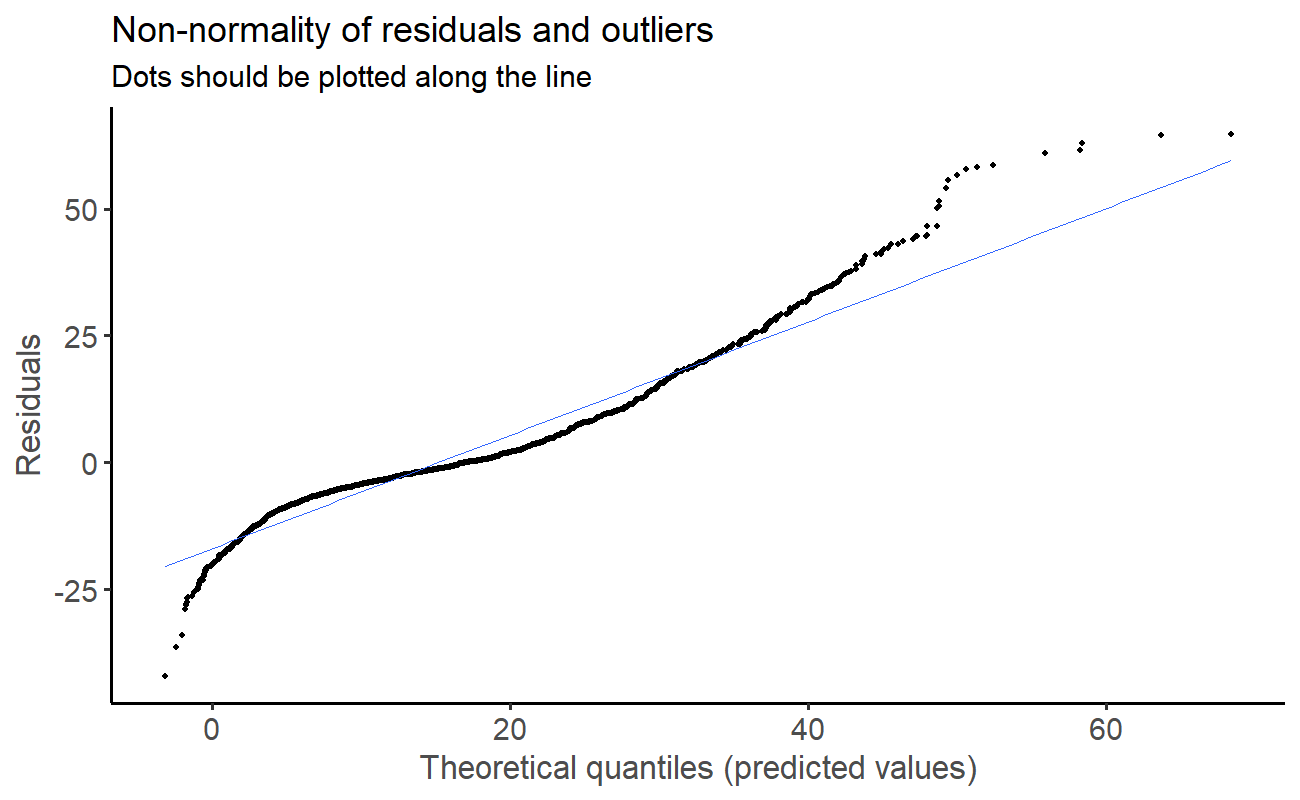
\includegraphics[width=0.5\linewidth]{C:/Users/keana/OneDrive - PennO365/Comp_transfer2018/Penn/stats_masters/stats-masters/figs/asm_mod3.1} 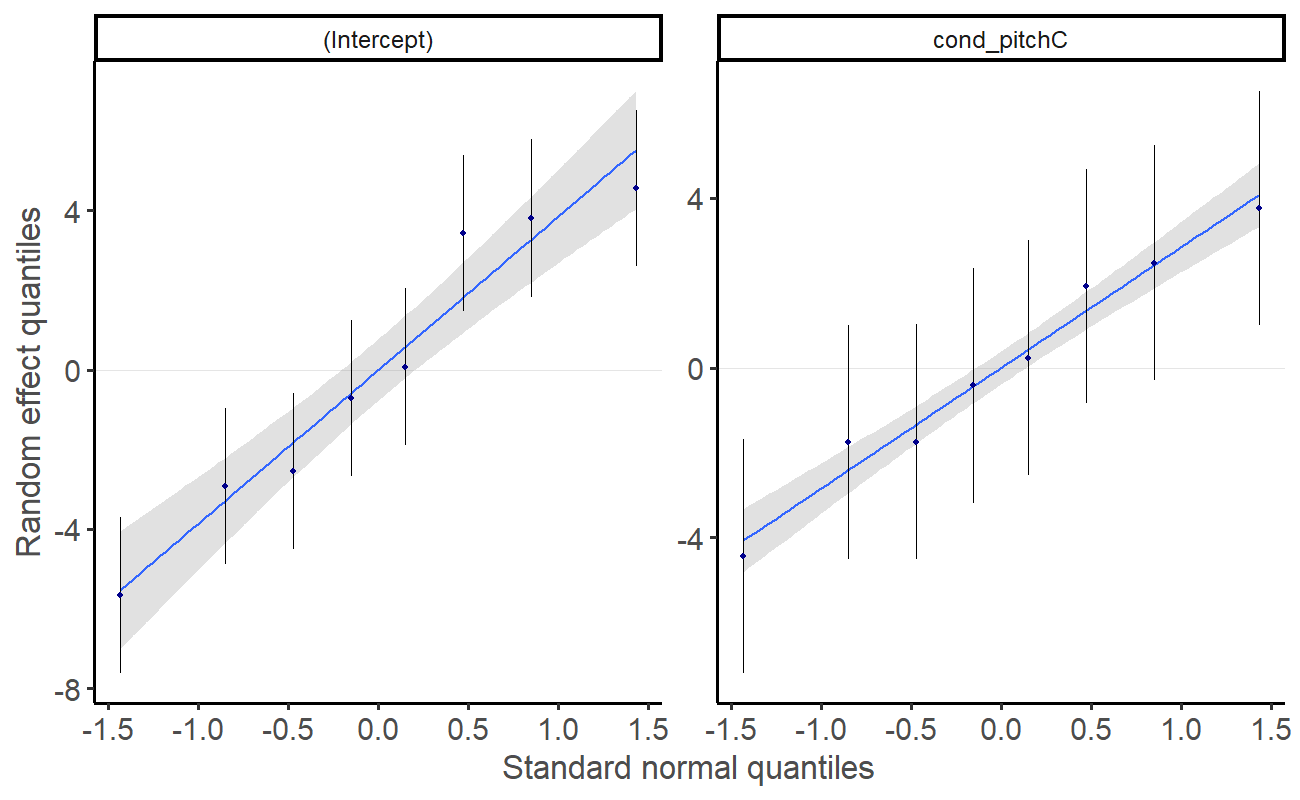
\includegraphics[width=0.5\linewidth]{C:/Users/keana/OneDrive - PennO365/Comp_transfer2018/Penn/stats_masters/stats-masters/figs/asm_mod3.2} 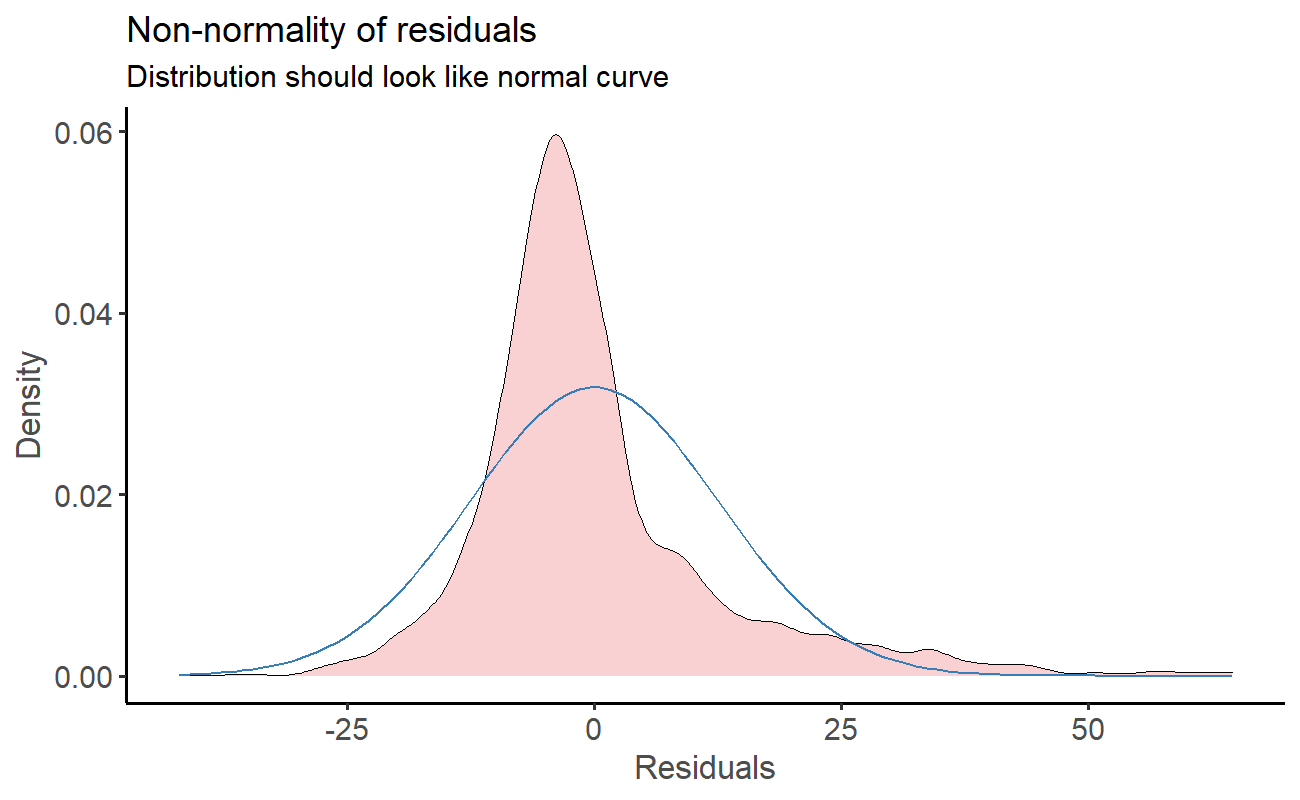
\includegraphics[width=0.5\linewidth]{C:/Users/keana/OneDrive - PennO365/Comp_transfer2018/Penn/stats_masters/stats-masters/figs/asm_mod3.3} 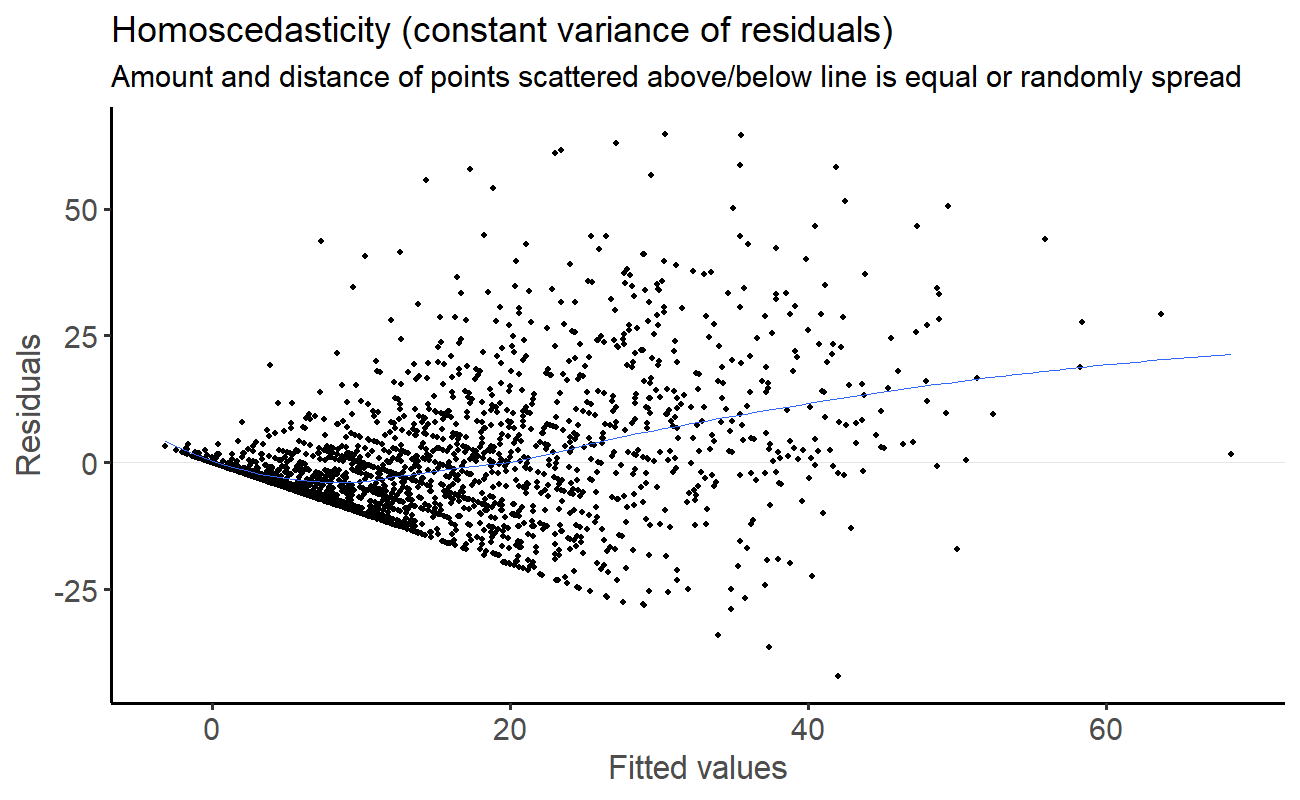
\includegraphics[width=0.5\linewidth]{C:/Users/keana/OneDrive - PennO365/Comp_transfer2018/Penn/stats_masters/stats-masters/figs/asm_mod3.4} \caption{Assumptions for Model 3: Trustworthiness and dominance predicting threat. The assumptions of normality and homoscedasticity for this model do not appear to have been met, with a relatively non-normal distribution of the residuals and a pattern in the plot showing fitted values against the residuals where there appears to be a sharp cut-off among the lower values of the plot. Thus, readers should compare the results from the final model to the robust version of the model to see if they replicate.}\label{fig:f19}
\end{figure}

\begin{figure}
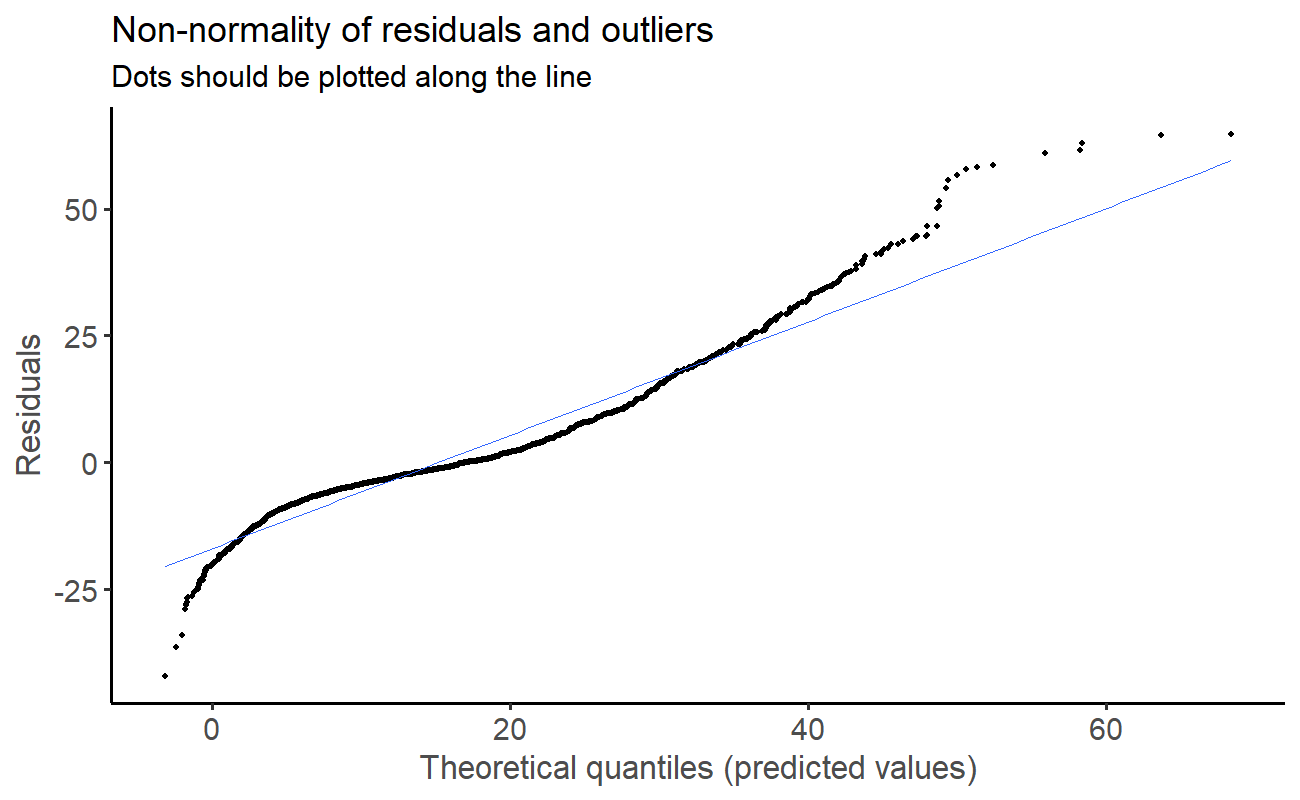
\includegraphics[width=0.5\linewidth]{C:/Users/keana/OneDrive - PennO365/Comp_transfer2018/Penn/stats_masters/stats-masters/figs/asm_mod5.1} 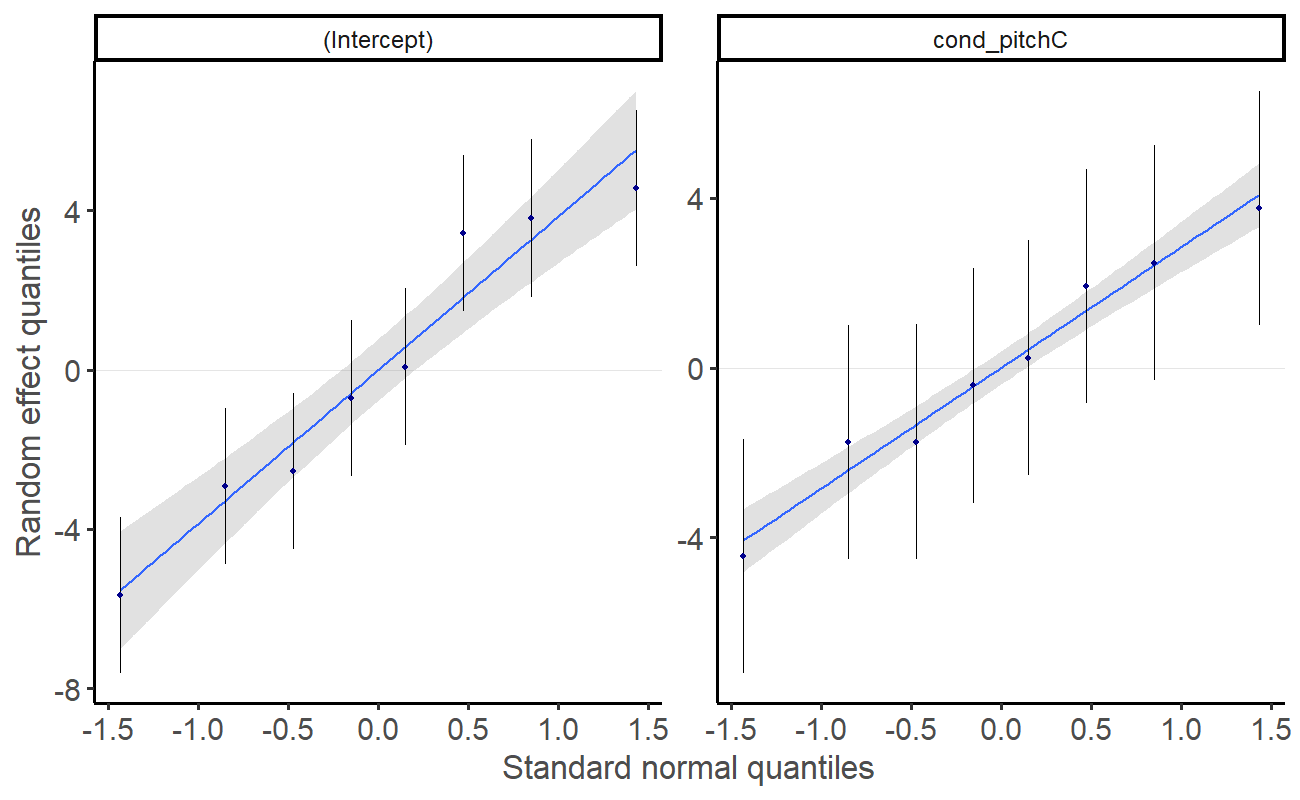
\includegraphics[width=0.5\linewidth]{C:/Users/keana/OneDrive - PennO365/Comp_transfer2018/Penn/stats_masters/stats-masters/figs/asm_mod5.2} 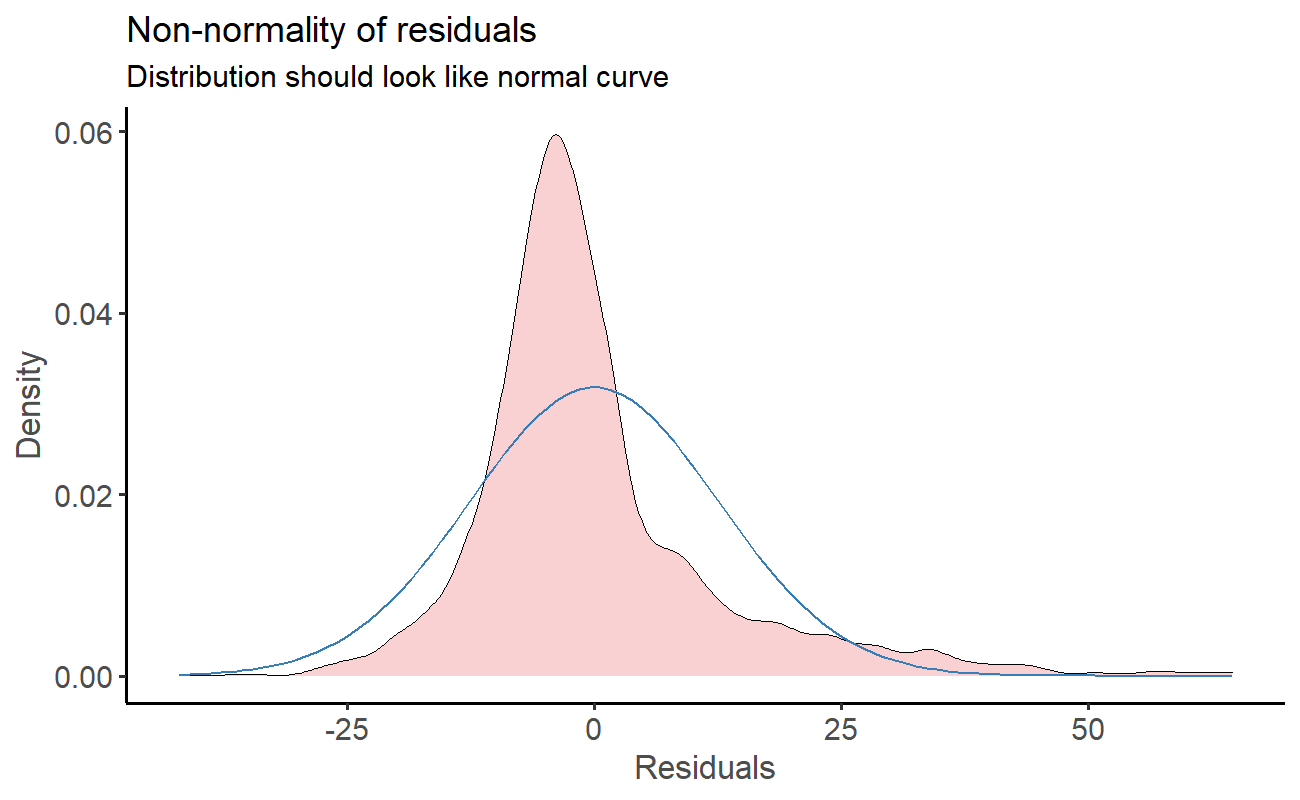
\includegraphics[width=0.5\linewidth]{C:/Users/keana/OneDrive - PennO365/Comp_transfer2018/Penn/stats_masters/stats-masters/figs/asm_mod5.3} 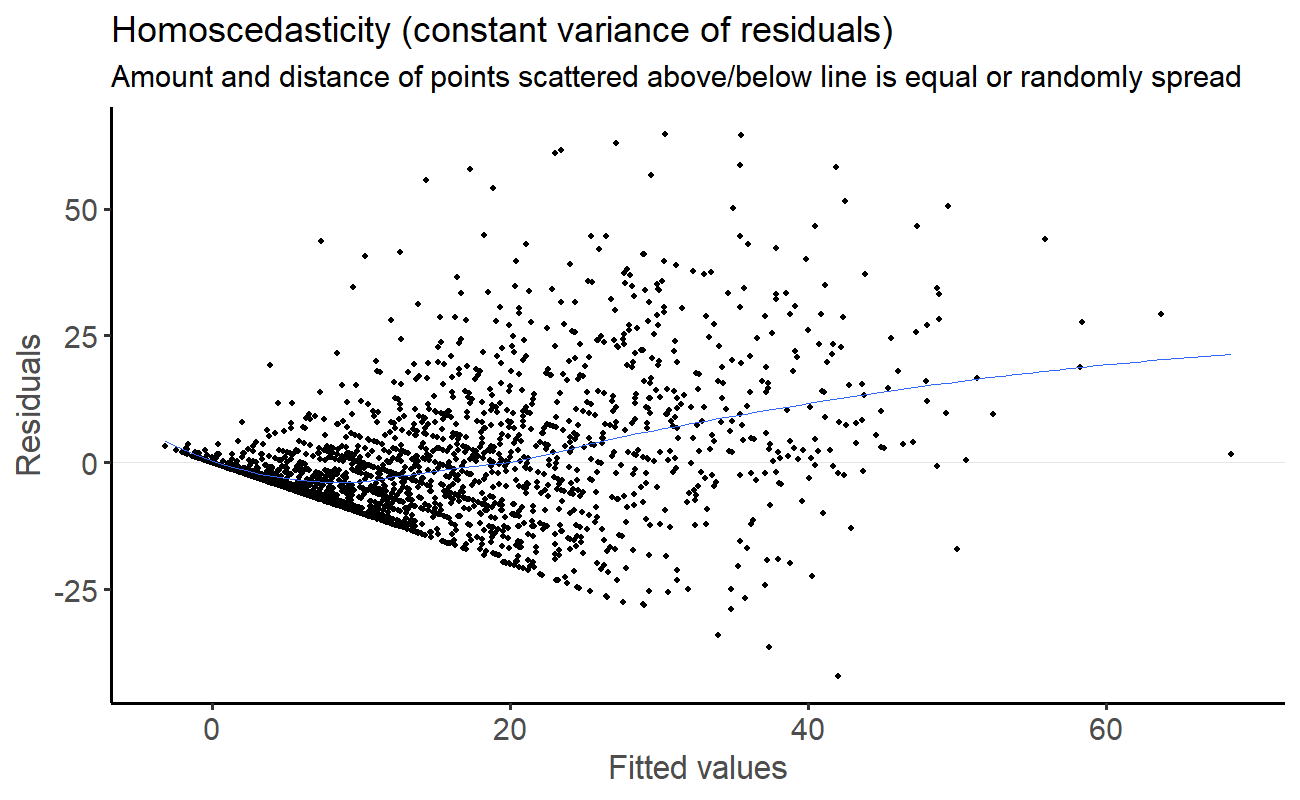
\includegraphics[width=0.5\linewidth]{C:/Users/keana/OneDrive - PennO365/Comp_transfer2018/Penn/stats_masters/stats-masters/figs/asm_mod5.4} \caption{Assumptions for Model 4: Effects of race on perceived trustworthiness. The assumptions of normality and homoscedasticity do not appear to have been met. There is not a linear relationship between the predicted values and the residuals, and there does not appear to be constant variance of the residuals. Thus, we encourage readers to refer to the robust model as a point of comparison.}\label{fig:f20}
\end{figure}

\begin{figure}
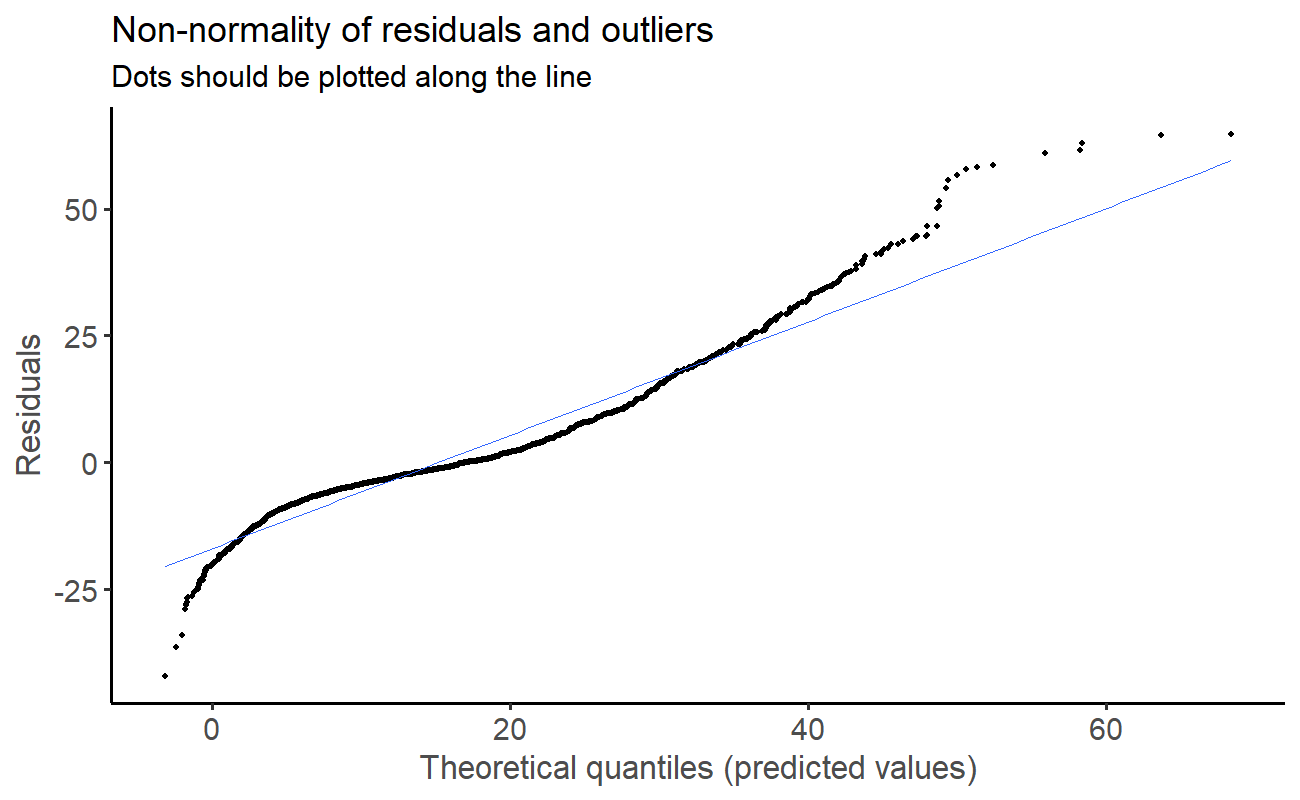
\includegraphics[width=0.5\linewidth]{C:/Users/keana/OneDrive - PennO365/Comp_transfer2018/Penn/stats_masters/stats-masters/figs/asm_mod6.1} 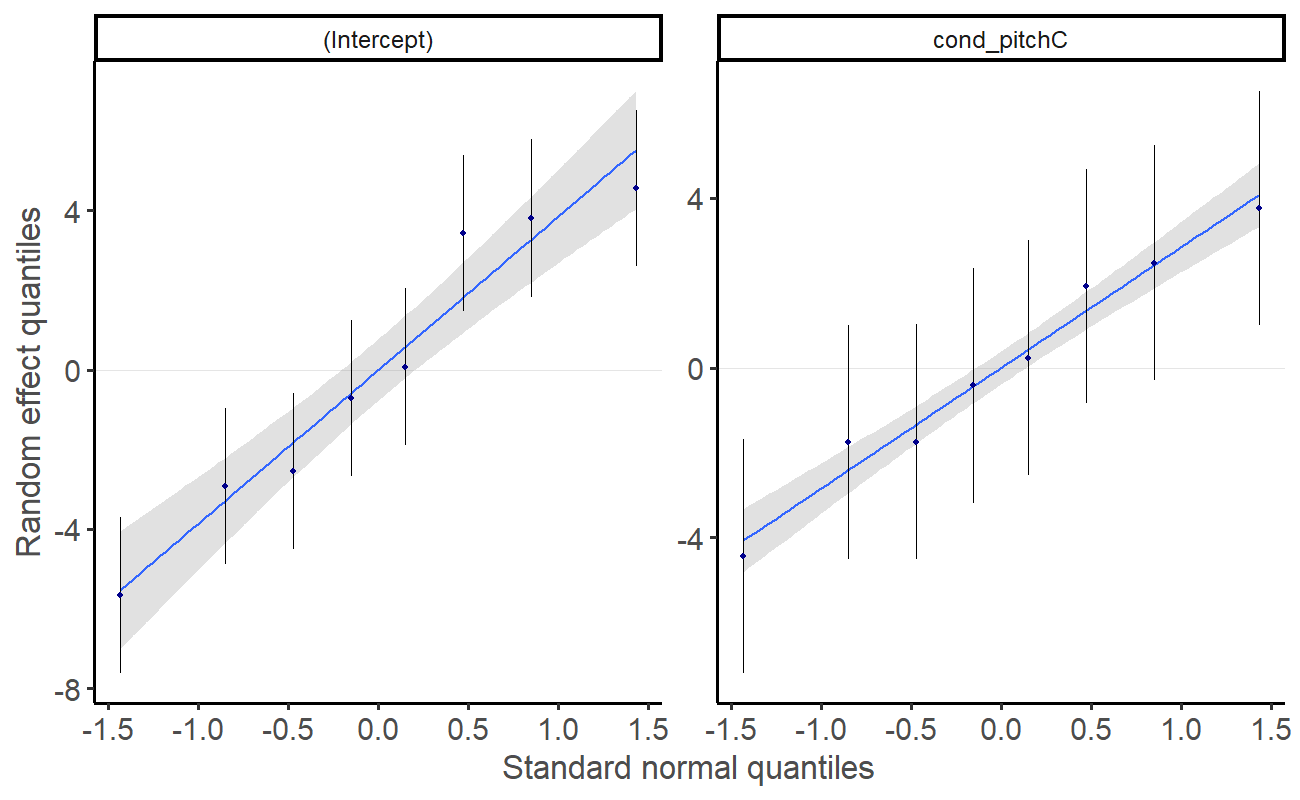
\includegraphics[width=0.5\linewidth]{C:/Users/keana/OneDrive - PennO365/Comp_transfer2018/Penn/stats_masters/stats-masters/figs/asm_mod6.2} 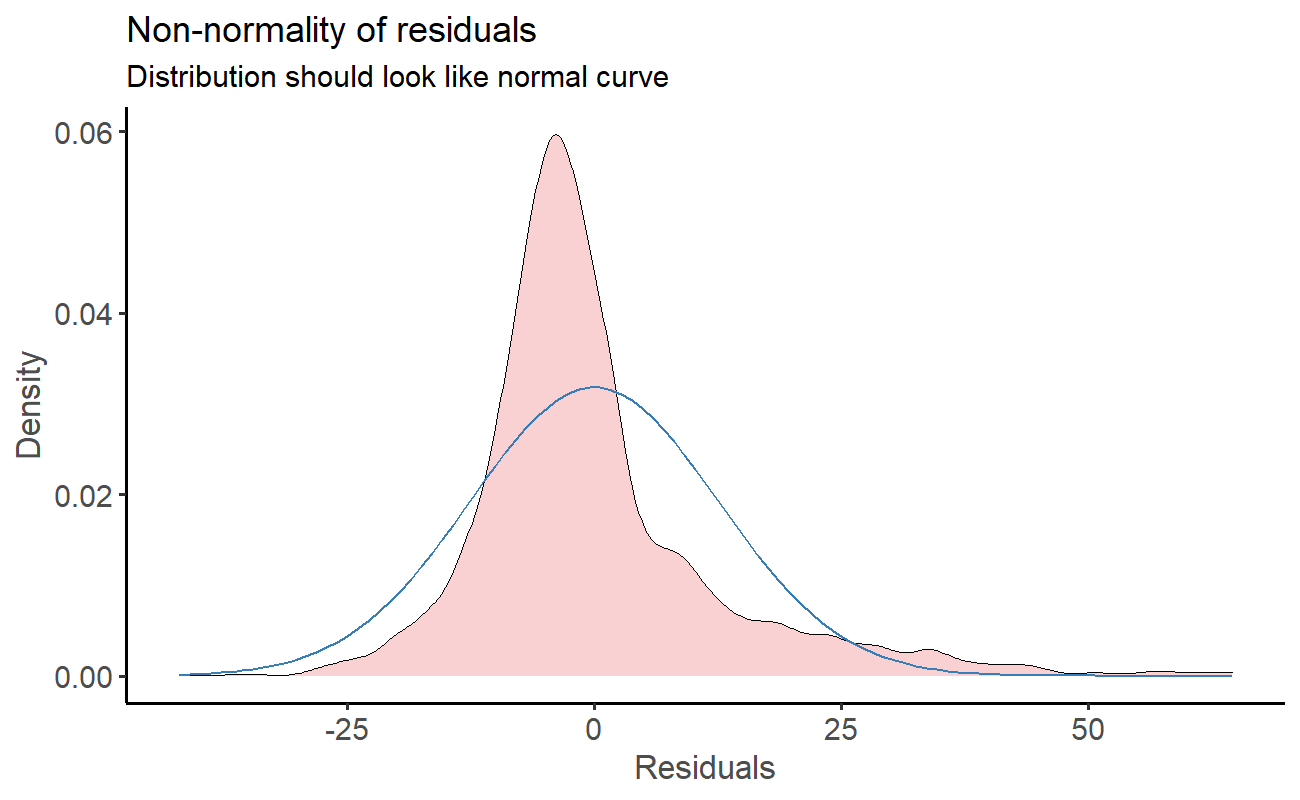
\includegraphics[width=0.5\linewidth]{C:/Users/keana/OneDrive - PennO365/Comp_transfer2018/Penn/stats_masters/stats-masters/figs/asm_mod6.3} 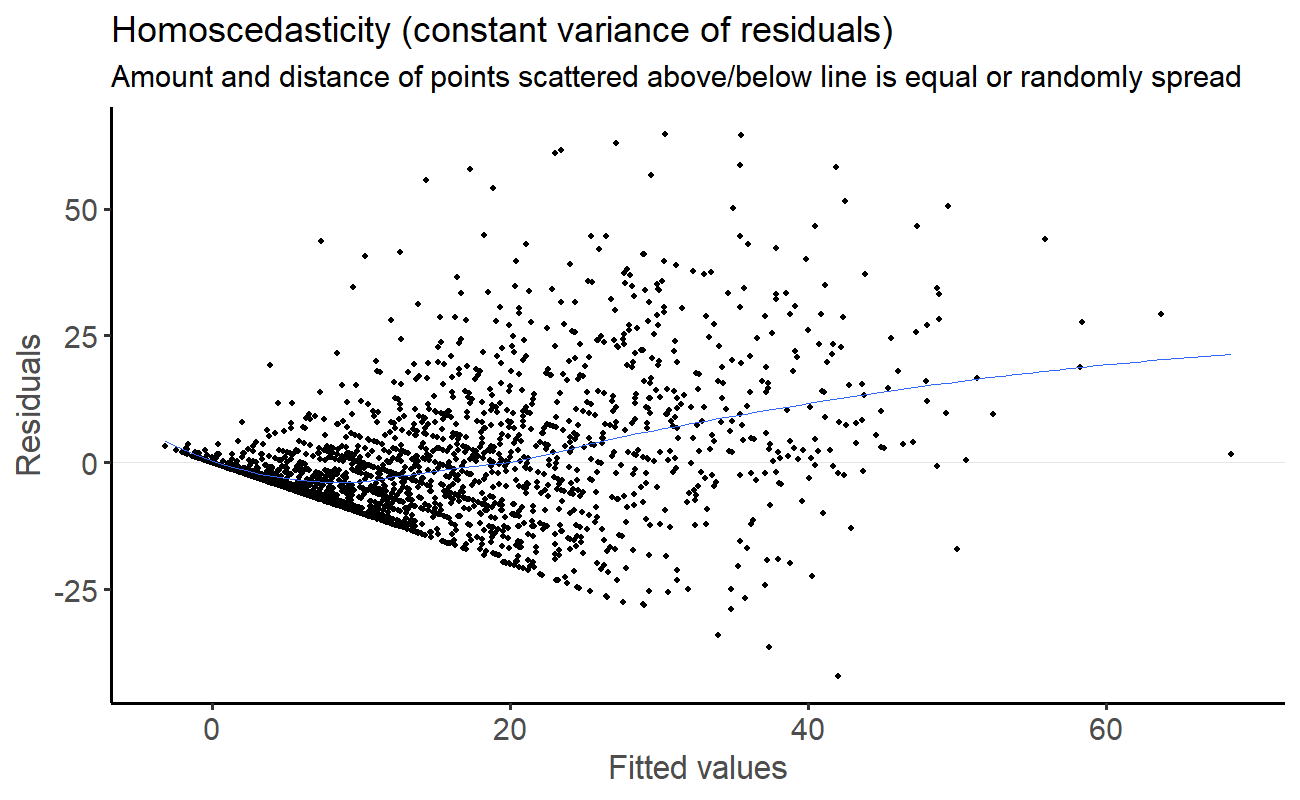
\includegraphics[width=0.5\linewidth]{C:/Users/keana/OneDrive - PennO365/Comp_transfer2018/Penn/stats_masters/stats-masters/figs/asm_mod6.4} \caption{Assumptions for Model 5: Effects of voice pitch on perceived dominance. Readers should compare the effects from the robust version of the model to the effects shown in the final models, since the assumptions of normality and homoscedasticity do not appear to have been met, with a the residuals following a non-normal distribution in the plot comparing the distribution of residuals to the normal distribution and the points in the plot checking homoscedasticity showing a pattern in the variation of the residuals.}\label{fig:f21}
\end{figure}

\begin{figure}
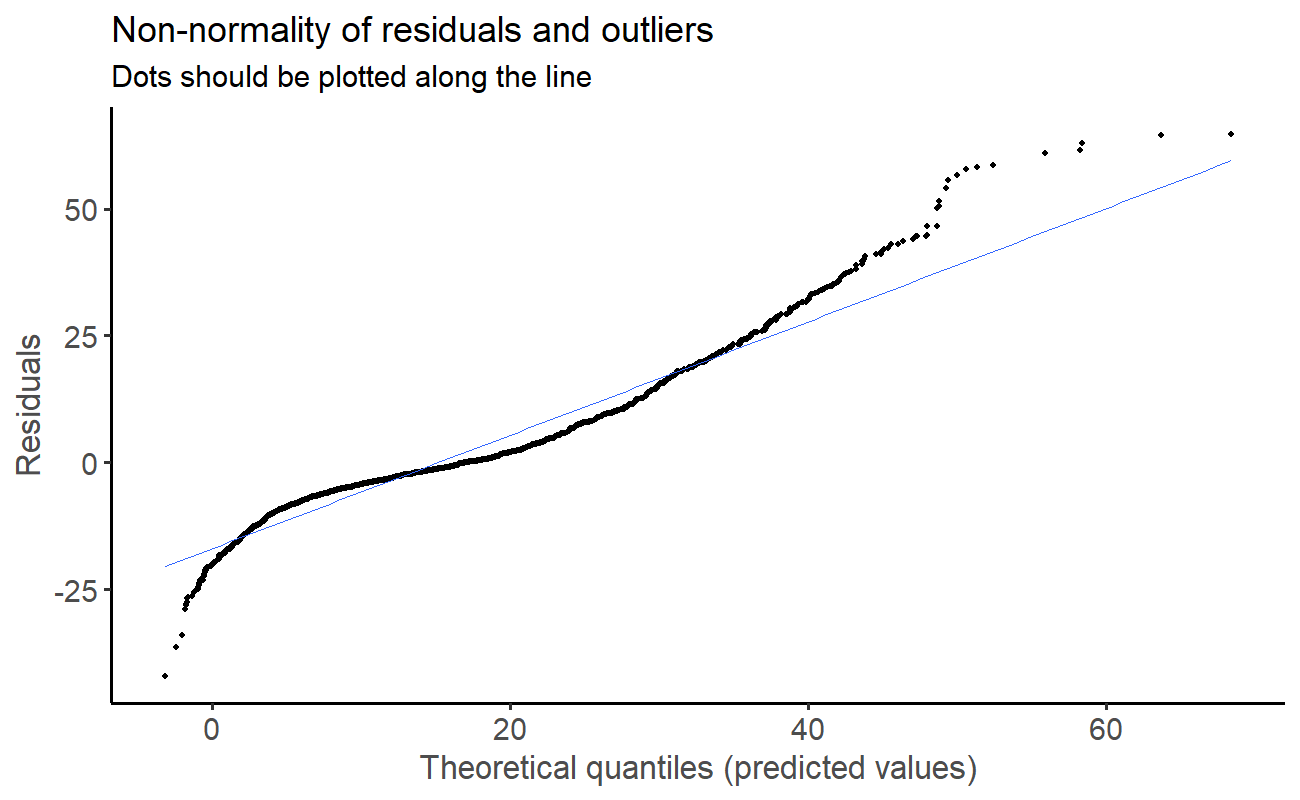
\includegraphics[width=0.5\linewidth]{C:/Users/keana/OneDrive - PennO365/Comp_transfer2018/Penn/stats_masters/stats-masters/figs/asm_mod7.1} 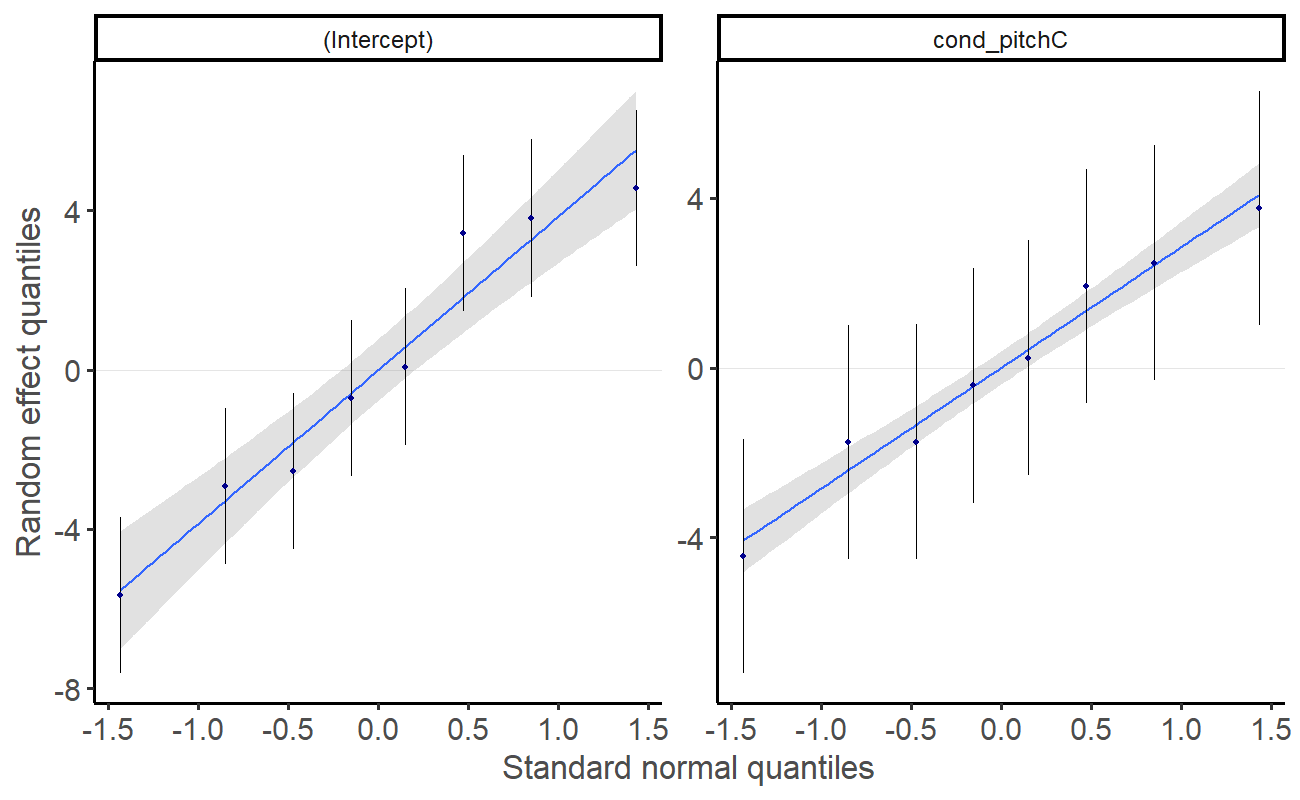
\includegraphics[width=0.5\linewidth]{C:/Users/keana/OneDrive - PennO365/Comp_transfer2018/Penn/stats_masters/stats-masters/figs/asm_mod7.2} 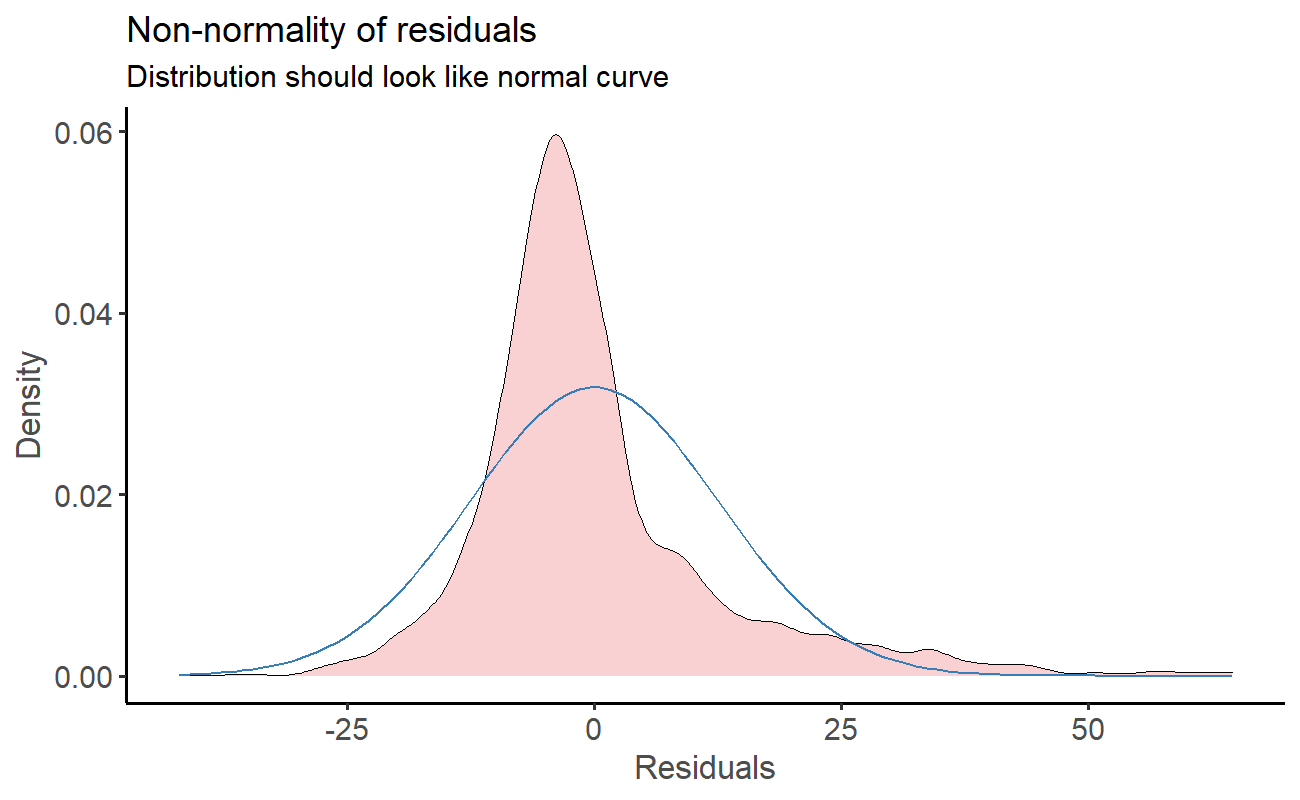
\includegraphics[width=0.5\linewidth]{C:/Users/keana/OneDrive - PennO365/Comp_transfer2018/Penn/stats_masters/stats-masters/figs/asm_mod7.3} 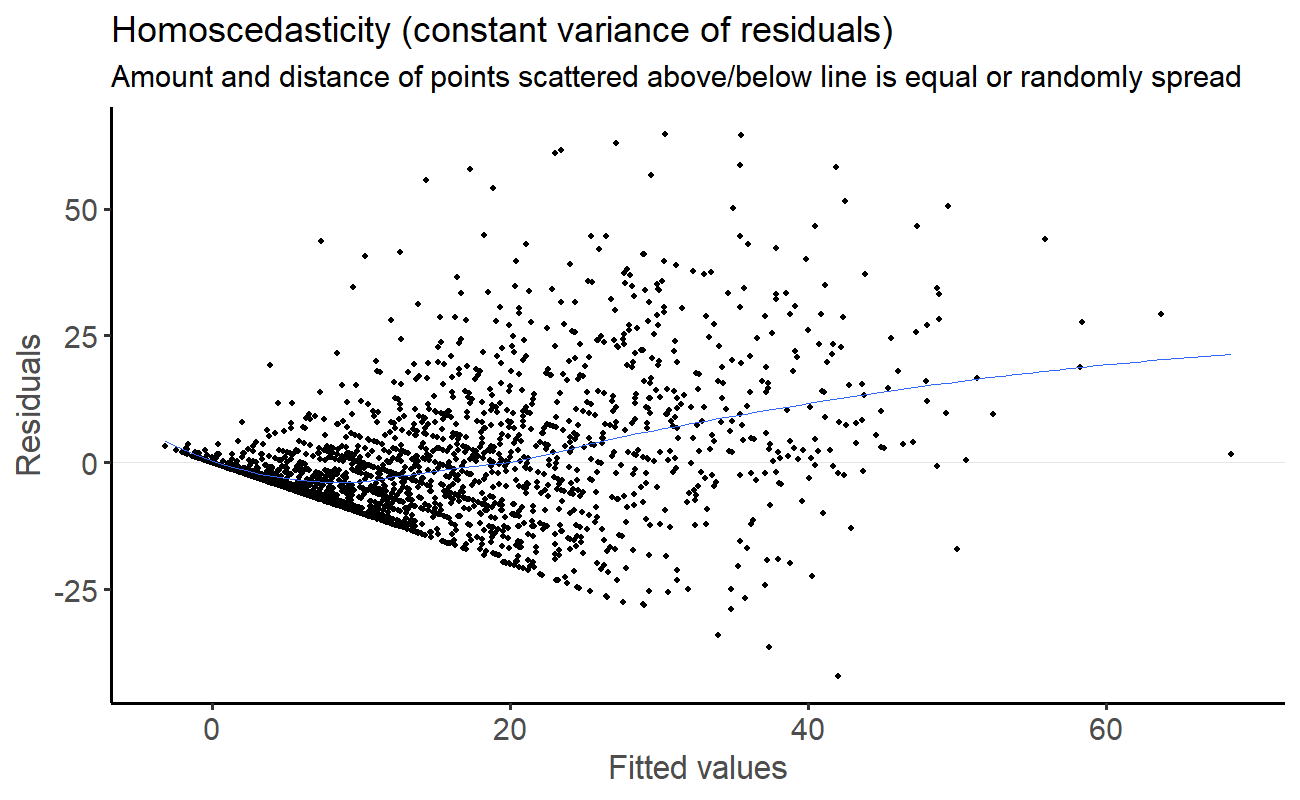
\includegraphics[width=0.5\linewidth]{C:/Users/keana/OneDrive - PennO365/Comp_transfer2018/Penn/stats_masters/stats-masters/figs/asm_mod7.4} \caption{Assumptions for Model 6: Effects of voice pitch and race on perceived threat potential. Based on these plots, the assumptions of homoscedasticity and normality of residuals do not appear to have been met. The upper left-hand plot shows that there is not a linear relationship between the residuals and predicted values. Additionally, the plot comparing the fitted values to the residuals checking shows heteroscedasticity in the variance of the residuals. Readers are encouraged to refer to the robust versions of the final model as a point of comparison.}\label{fig:f22}
\end{figure}

\hypertarget{software-references}{%
\subsection{Software references}\label{software-references}}

We used the following for analyses and write-up: R (Version 4.0.3; R Core Team, 2020) and the R-packages \emph{broom.mixed} (Version 0.2.6; Bolker \& Robinson, 2020), \emph{buildmer} (Version 1.7.1; Voeten, 2020), \emph{conflicted} (Version 1.0.4; Wickham, 2019a), \emph{data.table} (Version 1.13.0; Dowle \& Srinivasan, 2020), \emph{devtools} (Version 2.3.2; Wickham et al., 2020), \emph{ggplot2} (Version 3.3.2; Wickham, Chang, et al., 2020), \emph{gt} (Version 0.2.2; Iannone, Cheng, \& Schloerke, 2020; D. D. Sjoberg et al., 2020), \emph{gtsummary} (Version 1.3.5; Sjoberg et al., 2020), \emph{hablar} (Version 0.3.0; D. Sjoberg, 2020), \emph{here} (Version 0.1; Müller, 2017), \emph{knitr} (Version 1.30; Xie, 2020), \emph{lme4} (Version 1.1.23; Bates, Maechler, Bolker, \& Walker, 2020), \emph{lmerTest} (Version 3.1.2; Kuznetsova et al., 2020), \emph{memisc} (Version 0.99.25.6; Elff, 2020), \emph{nlme} (Version 3.1.149; Pinheiro, Bates, \& R-core, 2020), \emph{officer} (Version 0.3.14; Gohel, 2020), \emph{papaja} (Version 0.1.0.9997; Aust \& Barth, 2020), \emph{plm} (Version 2.2.4; Croissant et al., 2020), \emph{readr} (Version 1.4.0; Wickham \& Hester, 2020), \emph{reshape} (Version 0.8.8; Wickham, 2018), \emph{robustlmm} (Version 2.3; Koller, 2019), \emph{sjlabelled} (Version 1.1.7; Lüdecke, 2020a), \emph{sjmisc} (Version 2.8.5; Lüdecke, 2020b), \emph{sjPlot} (Version 2.8.5; Lüdecke, 2020c), \emph{snakecase} (Version 0.11.0; Grosser, 2019), \emph{summarytools} (Version 0.9.6; Comtois, 2020), \emph{tidyverse} (Version 1.3.0; Wickham, 2019b), \emph{webshot} (Version 0.5.2; Chang, 2019), and \emph{xtable} (Version 1.8.4; Dahl, Scott, Roosen, Magnusson, \& Swinton, 2019).

\newpage

\hypertarget{references}{%
\section{References}\label{references}}

\begingroup
\setlength{\parindent}{-0.5in}
\setlength{\leftskip}{0.5in}

\hypertarget{refs}{}
\begin{cslreferences}
\leavevmode\hypertarget{ref-Antonakis2019}{}%
Antonakis, J., Bastardoz, N., \& Ronkko, M. (2019). On ignoring the random effects assumption in multilevel models: Review, critique, and recommendations. \emph{Organizational Research Methods}. \url{https://doi.org/10.1177/1094428119877457}

\leavevmode\hypertarget{ref-Apicella2009}{}%
Apicella, C. L., \& Feinberg, D. R. (2009). Voice pitch alters mate-choice-relevant perception in hunter-gatherers. \emph{Proceedings of the Royal Society B: Biological Sciences}, \emph{276}, 1077--1082. \url{https://doi.org/10.1098/rspb.2008.1542}

\leavevmode\hypertarget{ref-R-papaja}{}%
Aust, F., \& Barth, M. (2020). \emph{Papaja: Prepare reproducible apa journal articles with r markdown}. Retrieved from \url{https://github.com/crsh/papaja}

\leavevmode\hypertarget{ref-Ayres2015}{}%
Ayres, I., Banaji, M., \& Jolls, C. (2015). Race effects on eBay. \emph{RAND Journal of Economics}, \emph{46}(4), 891--917. \url{https://doi.org/10.1111/1756-2171.12115}

\leavevmode\hypertarget{ref-Baayen2008}{}%
Baayen, R. H., Davidson, D. J., \& Bates, D. M. (2008). Mixed-effects modeling with crossed random effects for subjects and items. \emph{Journal of Memory and Language}, \emph{59}(4), 390--412. \url{https://doi.org/10.1016/j.jml.2007.12.005}

\leavevmode\hypertarget{ref-Barr2013}{}%
Barr, D., Levy, R., Scheepers, C., \& Tily, H. J. (2013). Random effects structure for confirmatory hypothesis testing: Keep it maximal. \emph{Journal of Memory and Language}, \emph{68}(3), 1--43. \url{https://doi.org/10.1016/j.jml.2012.11.001.Random}

\leavevmode\hypertarget{ref-Bates2015}{}%
Bates, D., Kliegl, R., Vasishth, S., \& Baayen, H. (2015). Parsimonious mixed models. Retrieved from \url{http://arxiv.org/abs/1506.04967}

\leavevmode\hypertarget{ref-R-lme4}{}%
Bates, D., Maechler, M., Bolker, B., \& Walker, S. (2020). \emph{Lme4: Linear mixed-effects models using eigen and s4}. Retrieved from \url{https://github.com/lme4/lme4/}

\leavevmode\hypertarget{ref-Biernat2003}{}%
Biernat, M. (2003). Toward a broader view of social stereotyping. \emph{American Psychologist}, \emph{58}(12), 1019--1027. \url{https://doi.org/10.1037/0003-066X.58.12.1019}

\leavevmode\hypertarget{ref-Biernat1991}{}%
Biernat, M., Manis, M., \& Nelson, T. E. (1991). Stereotypes and standards of judgment. \emph{Journal of Personality and Social Psychology}, \emph{60}(4), 485--499. \url{https://doi.org/10.1037/0022-3514.60.4.485}

\leavevmode\hypertarget{ref-Boersma2001}{}%
Boersma, P., \& Heuven, V. van. (2001). Speak and unSpeak with Praat. \emph{Glot International}, \emph{5}(9-10), 341--347.

\leavevmode\hypertarget{ref-R-broom.mixed}{}%
Bolker, B., \& Robinson, D. (2020). \emph{Broom.mixed: Tidying methods for mixed models}. Retrieved from \url{http://github.com/bbolker/broom.mixed}

\leavevmode\hypertarget{ref-Bowles2009}{}%
Bowles, S. (2009). Did warfare among ancestral hunter-gatherer affect the evolution of human social behaviors? \emph{Science}, \emph{324}, 1293--1298. Retrieved from \url{http://science.sciencemag.org/content/324/5932/1293.short}

\leavevmode\hypertarget{ref-Brauer2018}{}%
Brauer, M., \& Curtin, J. J. (2018). Linear mixed-effects models and the analysis of nonindependent data: A unified framework to analyze categorical and continuous independent variables that vary within-subjects and/or within-items. \emph{Psychological Methods}, \emph{23}(3), 389--411.

\leavevmode\hypertarget{ref-Browne2006}{}%
Browne, W. J., \& Draper, D. (2006). A comparison of Bayesian and likelihood-based methods for fitting multilevel models. \emph{Bayesian Analysis}, \emph{1}(3), 473--514. \url{https://doi.org/10.1214/06-BA117}

\leavevmode\hypertarget{ref-R-webshot}{}%
Chang, W. (2019). \emph{Webshot: Take screenshots of web pages}. Retrieved from \url{https://github.com/wch/webshot/}

\leavevmode\hypertarget{ref-Clarke2007}{}%
Clarke, P., \& Wheaton, B. (2007). Addressing data sparseness in contextual population research using cluster analysis to create synthetic neighborhoods. \emph{Sociological Methods \& Research}, \emph{35}(3), 311--351.

\leavevmode\hypertarget{ref-R-summarytools}{}%
Comtois, D. (2020). \emph{Summarytools: Tools to quickly and neatly summarize data}. Retrieved from \url{https://github.com/dcomtois/summarytools}

\leavevmode\hypertarget{ref-Correll2007}{}%
Correll, J., Park, B., Judd, C. M., \& Wittenbrink, B. (2007). The influence of stereotypes on decisions to shoot. \emph{European Journal of Social Psychology}, \emph{37}, 1102--1117. \url{https://doi.org/10.1002/ejsp}

\leavevmode\hypertarget{ref-Cottrell2005}{}%
Cottrell, C. A., \& Neuberg, S. L. (2005). Different emotional reactions to different groups: A sociofunctional threat-based approach to "prejudice". \emph{Journal of Personality and Social Psychology}, \emph{88}(5), 770--789. \url{https://doi.org/10.1037/0022-3514.88.5.770}

\leavevmode\hypertarget{ref-R-plm}{}%
Croissant, Y., Millo, G., \& Tappe, K. (2020). \emph{Plm: Linear models for panel data}. Retrieved from \url{https://CRAN.R-project.org/package=plm}

\leavevmode\hypertarget{ref-R-xtable}{}%
Dahl, D. B., Scott, D., Roosen, C., Magnusson, A., \& Swinton, J. (2019). \emph{Xtable: Export tables to latex or html}. Retrieved from \url{http://xtable.r-forge.r-project.org/}

\leavevmode\hypertarget{ref-Devine1995}{}%
Devine, P. G., \& Elliot, A. J. (1995). Are Racial Stereotypes Really Fading? The Princeton Trilogy Revisited. \emph{Personality and Social Psychology Bulletin}, \emph{21}(11), 1139--1150.

\leavevmode\hypertarget{ref-Dixon2007}{}%
Dixon, T. L., \& Azocar, C. L. (2007). Priming crime and activating blackness: Understanding the psychological impact of the overrepresentation of blacks as lawbreakers on television news. \emph{Journal of Communication}, \emph{57}(2), 229--253. \url{https://doi.org/10.1111/j.1460-2466.2007.00341.x}

\leavevmode\hypertarget{ref-Doleac2013}{}%
Doleac, J. L., \& Stein, L. C. D. (2013). The visible hand: Race and online market outcomes. \emph{The Economic Journal}, \emph{123}(572), 1--18. \url{https://doi.org/10.1111/ecoj.12082}

\leavevmode\hypertarget{ref-R-data.table}{}%
Dowle, M., \& Srinivasan, A. (2020). \emph{Data.table: Extension of `data.frame`}. Retrieved from \url{https://CRAN.R-project.org/package=data.table}

\leavevmode\hypertarget{ref-Eberhardt2006}{}%
Eberhardt, J. L., Davies, P. G., Purdie-Vaughns, V. J., \& Johnson, S. L. (2006). Looking deathworthy perceived stereotypicality of black defendants predicts capital-sentencing outcomes. \emph{Psychological Science}, \emph{17}(5), 383--386. \url{https://doi.org/10.1111/j.1467-9280.2006.01716.x}

\leavevmode\hypertarget{ref-R-memisc}{}%
Elff, M. (2020). \emph{Memisc: Management of survey data and presentation of analysis results}. Retrieved from \url{https://CRAN.R-project.org/package=memisc}

\leavevmode\hypertarget{ref-Elff2020}{}%
Elff, M., Heisig, J. P., Schaeffer, M., \& Shikano, S. (2020). Multilevel analysis with few clusters: Improving likelihood-based methods to provide unbiased estimates and accurate inference. \emph{British Journal of Political Science}, 1--15. \url{https://doi.org/10.1017/S0007123419000097}

\leavevmode\hypertarget{ref-Fairbanks1960}{}%
Fairbanks, G. (1960). \emph{Voice and articulation drillbook}. New York, NY: Harper.

\leavevmode\hypertarget{ref-Feinberg2005}{}%
Feinberg, D. R., Jones, B. C., Little, A. C., Burt, D. M., \& Perrett, D. I. (2005). Manipulations of fundamental and formant frequencies influence the attractiveness of human male voices. \emph{Animal Behaviour}, \emph{69}(3), 561--568. \url{https://doi.org/10.1016/j.anbehav.2004.06.012}

\leavevmode\hypertarget{ref-Finch2014}{}%
Finch, W. H., Bolin, J. E., \& Kelley, K. (2014). \emph{Multilevel modeling using R}.

\leavevmode\hypertarget{ref-Fraccaro2011}{}%
Fraccaro, P. J., Jones, B. C., Vukovic, J., Smith, F. G., Watkins, C. D., Feinberg, D. R., \ldots{} Debruine, L. M. (2011). Experimental evidence that women speak in a higher voice pitch to men they find attractive. \emph{Journal of Evolutionary Psychology}, \emph{9}(1), 57--67. \url{https://doi.org/10.1556/JEP.9.2011.33.1}

\leavevmode\hypertarget{ref-Fraccaro2013}{}%
Fraccaro, P. J., O'Connor, J. J. M., Re, D. E., Jones, B. C., DeBruine, L. M., \& Feinberg, D. R. (2013). Faking it: Deliberately altered voice pitch and vocal attractiveness. \emph{Animal Behaviour}, \emph{85}(1), 127--136. \url{https://doi.org/10.1016/j.anbehav.2012.10.016}

\leavevmode\hypertarget{ref-Gaddis2017}{}%
Gaddis, S. (2017). How Black are Lakisha and Jamal? Racial perceptions from names used in correspondence audit studies. \emph{Sociological Science}, \emph{4}, 469--489. \url{https://doi.org/10.15195/v4.a19}

\leavevmode\hypertarget{ref-Galecki2013}{}%
Galecki, A., \& Burzykowski, T. (2013). \emph{Linear mixed-effects models using R: A step-by-step approach}.

\leavevmode\hypertarget{ref-Garson2013}{}%
Garson, G. D. (2013). \emph{Hierarchical linear modeling: Guide and applications}.

\leavevmode\hypertarget{ref-Gelman2007}{}%
Gelman, A., \& Hill, J. (2007). \emph{Data analysis using regression and multilevel/hierarchical models}.

\leavevmode\hypertarget{ref-Gilliam1996}{}%
Gilliam, F. D., Iyengar, S., Simon, A., \& Wright, O. (1996). Crime in black and white: The violent, scary world of local news. \emph{Harvard International Journal of Press/Politics}, \emph{1}(3), 6--23. \url{https://doi.org/10.1177/1081180X96001003003}

\leavevmode\hypertarget{ref-R-officer}{}%
Gohel, D. (2020). \emph{Officer: Manipulation of microsoft word and powerpoint documents}. Retrieved from \url{https://davidgohel.github.io/officer/}

\leavevmode\hypertarget{ref-R-snakecase}{}%
Grosser, M. (2019). \emph{Snakecase: Convert strings into any case}. Retrieved from \url{https://github.com/Tazinho/snakecase}

\leavevmode\hypertarget{ref-Harries1998}{}%
Harries, M., Hawkins, S., Hacking, J., \& Hughes, I. (1998). Changes in the male voice at puberty: vocal fold length and its relationship to the fundamental frequency of the voice. \emph{The Journal of Laryngology and Otology}, \emph{112}, 451--454.

\leavevmode\hypertarget{ref-Hausman1978}{}%
Hausman, J. (1978). Specification tests in econometrics. \emph{Econometrica}, \emph{46}(6), 1251--1271. Retrieved from \url{http://www.jstor.org/stable/1913827\%7B/\%\%7D5Cnhttp://www.jstor.org/\%7B/\%\%7D5Cnhttp://www.jstor.org/action/showPublisher?publisherCode=econosoc.\%7B/\%\%7D5Cnhttp://www.jstor.org}

\leavevmode\hypertarget{ref-Hayward2000}{}%
Hayward, M. D., Miles, T. P., Crimmins, E. M., \& Yang, Y. (2000). The significance of socioeconomic status in explaining the racial gap in chronic health conditions. \emph{American Sociological Review}, \emph{65}(6), 910--930.

\leavevmode\hypertarget{ref-Hester2018}{}%
Hester, N., \& Gray, K. (2018). For Black men, being tall increases threat stereotyping and police stops. \emph{Proceedings of the National Academy of Sciences}, \emph{115}(11), 2711--2715. \url{https://doi.org/10.1073/pnas.1714454115}

\leavevmode\hypertarget{ref-Hodges-Simeon2015}{}%
Hodges-Simeon, C. R., Gurven, M., \& Gaulin, S. J. C. (2015). The low male voice is a costly signal of phenotypic quality among Bolivian adolescents. \emph{Evolution and Human Behavior}, \emph{36}(4), 1--9. \url{https://doi.org/10.1016/j.evolhumbehav.2015.01.002}

\leavevmode\hypertarget{ref-Hodges-Simeon2014}{}%
Hodges-Simeon, C. R., Gurven, M., Puts, D., \& Gaulin, S. (2014). Vocal fundamental and formant frequencies are honest signals of threat potential in peripubertal males. \emph{Behavioral Ecology}, \emph{25}(4), 984--988. \url{https://doi.org/10.1093/beheco/aru081}

\leavevmode\hypertarget{ref-Hox2020}{}%
Hox, J., \& McNeish, D. (2020). Small samples in multilevel modeling. In \emph{Small sample size solutions} (pp. 215--225).

\leavevmode\hypertarget{ref-Hughes2014}{}%
Hughes, S. M., Mogilski, J. K., \& Harrison, M. A. (2014). The perception and parameters of intentional voice manipulation. \emph{Journal of Nonverbal Behavior}, \emph{38}(1), 107--127. \url{https://doi.org/10.1007/s10919-013-0163-z}

\leavevmode\hypertarget{ref-R-gt}{}%
Iannone, R., Cheng, J., \& Schloerke, B. (2020). \emph{Gt: Easily create presentation-ready display tables}. Retrieved from \url{https://github.com/rstudio/gt}

\leavevmode\hypertarget{ref-Judd2017}{}%
Judd, C. M., Westfall, J., \& Kenny, D. A. (2017). Experiments with more than one random factor: Designs, analytic models, and statistical power. \emph{Annual Review of Psychology}, \emph{68}, 17.1--17.25. \url{https://doi.org/10.1146/annurev-psych-122414-033702}

\leavevmode\hypertarget{ref-Kenward1997}{}%
Kenward, M. G., \& Roger, J. H. (1997). Small sample inference for fixed effects from restricted maximum likelihood. \emph{Biometrics}, \emph{53}(3), 983--997.

\leavevmode\hypertarget{ref-Kirkpatrick1991}{}%
Kirkpatrick, S. A., \& Locke, E. A. (1991). Leadership: Do traits matter? \emph{The Executive}, \emph{5}(2), 48--60. \url{https://doi.org/10.5465/AME.1991.4274679}

\leavevmode\hypertarget{ref-Klofstad2018}{}%
Klofstad, C. A., \& Anderson, R. C. (2018). Voice pitch predicts electability , but does not signal leadership ability. \emph{Evolution and Human Behavior}. \url{https://doi.org/10.1016/j.evolhumbehav.2018.02.007}

\leavevmode\hypertarget{ref-Klofstad2012}{}%
Klofstad, C. A., Anderson, R. C., \& Peters, S. (2012). Sounds like a winner: Voice pitch influences perception of leadership capacity in both men and women. \emph{Proceedings of the Royal Society B: Biological Sciences}, \emph{279}(1738), 2698--2704. \url{https://doi.org/10.1098/rspb.2012.0311}

\leavevmode\hypertarget{ref-Knuycky2014}{}%
Knuycky, L. R., Kleider, H. M., \& Cavrak, S. E. (2014). Line-up misidentifications: When being 'prototypically black' is perceived as criminal. \emph{Applied Cognitive Psychology}, \emph{28}(1), 39--46. \url{https://doi.org/10.1002/acp.2954}

\leavevmode\hypertarget{ref-Koller2016}{}%
Koller, M. (2016). robustlmm: An R Package for robust estimation of linear mixed-effects models. \emph{Journal of Statistical Software}, \emph{75}(6), 1--24.

\leavevmode\hypertarget{ref-R-robustlmm}{}%
Koller, M. (2019). \emph{Robustlmm: Robust linear mixed effects models}. Retrieved from \url{https://github.com/kollerma/robustlmm}

\leavevmode\hypertarget{ref-Koller2011}{}%
Koller, M., \& Stahel, W. A. (2011). Sharpening Wald-type inference in robust regression for small samples. \emph{Computational Statistics and Data Analysis}, \emph{55}(8), 2504--2515. \url{https://doi.org/10.1016/j.csda.2011.02.014}

\leavevmode\hypertarget{ref-Kreiman2011}{}%
Kreiman, J., \& Sidtis, D. (2011). \emph{Foundations of voice studies: An interdisciplinary approach to voice production and perception}.

\leavevmode\hypertarget{ref-Kurzban2001}{}%
Kurzban, R., \& Leary, M. R. (2001). Evolutionary origins of stigmatization: The functions of social exclusion. \emph{Psychological Bulletin}, \emph{127}(2), 187--208. \url{https://doi.org/10.1037/0033-2909.127.2.187}

\leavevmode\hypertarget{ref-R-lmerTest}{}%
Kuznetsova, A., Bruun Brockhoff, P., \& Haubo Bojesen Christensen, R. (2020). \emph{LmerTest: Tests in linear mixed effects models}. Retrieved from \url{https://github.com/runehaubo/lmerTestR}

\leavevmode\hypertarget{ref-Labov2010}{}%
Labov, W. (2010). Unendangered dialect, endangered people: The case of African American vernacular English. \emph{Transforming Anthropology}, \emph{18}(1), 15--28. \url{https://doi.org/10.1111/j.1548-7466.2010.01066.x.15}

\leavevmode\hypertarget{ref-Li2017}{}%
Li, N. P., Vugt, M. van, \& Colarelli, S. M. (2017). The Evolutionary Mismatch Hypothesis: Implications for Psychological Science. \emph{Current Directions in Psychological Science}, 096372141773137. \url{https://doi.org/10.1177/0963721417731378}

\leavevmode\hypertarget{ref-Livingston2009}{}%
Livingston, R. W., \& Pearce, N. A. (2009). The teddy-bear effect: Does having a baby face benefit black chief executive officers? \emph{Psychological Science}, \emph{20}(10), 1229--1236. \url{https://doi.org/10.1111/j.1467-9280.2009.02431.x}

\leavevmode\hypertarget{ref-Luke2017}{}%
Luke, S. G. (2017). Evaluating significance in linear mixed-effects models in R. \emph{Behavior Research Methods}, \emph{49}, 1494--1502. \url{https://doi.org/10.3758/s13428-016-0809-y}

\leavevmode\hypertarget{ref-R-sjlabelled}{}%
Lüdecke, D. (2020a). \emph{Sjlabelled: Labelled data utility functions}. Retrieved from \url{https://strengejacke.github.io/sjlabelled/}

\leavevmode\hypertarget{ref-R-sjmisc}{}%
Lüdecke, D. (2020b). \emph{Sjmisc: Data and variable transformation functions}. Retrieved from \url{https://strengejacke.github.io/sjmisc}

\leavevmode\hypertarget{ref-R-sjPlot}{}%
Lüdecke, D. (2020c). \emph{SjPlot: Data visualization for statistics in social science}. Retrieved from \url{https://strengejacke.github.io/sjPlot/}

\leavevmode\hypertarget{ref-Maas2004}{}%
Maas, C. J. M., \& Hox, J. J. (2004). The influence of violations of assumptions on multilevel parameter estimates and their standard errors. \emph{Computational Statistics and Data Analysis}, \emph{46}(3), 427--440. \url{https://doi.org/10.1016/j.csda.2003.08.006}

\leavevmode\hypertarget{ref-Maas2005}{}%
Maas, C. J. M., \& Hox, J. J. (2005). Sufficient sample sizes for multilevel modeling. \emph{Methodology}, \emph{1}(3), 86--92. \url{https://doi.org/10.1027/1614-1881.1.3.86}

\leavevmode\hypertarget{ref-Maner2005}{}%
Maner, J. K., Kenrick, D. T., Backer, D. V., Robertson, T. E., Hofer, B., Neuberg, S. L., \ldots{} Schaller, M. (2005). Functional projection: How fundamental social motives can bias interpersonal perception. \emph{Journal of Personality and Social Psychology}, \emph{88}(1), 63--78. \url{https://doi.org/10.1037/0022-3514.88.1.63}

\leavevmode\hypertarget{ref-Matuschek2017}{}%
Matuschek, H., Kliegl, R., Vasishth, S., Baayen, H., \& Bates, D. (2017). Balancing Type I error and power in linear mixed models. \emph{Journal of Memory and Language}, \emph{94}, 305--315. \url{https://doi.org/10.1016/j.jml.2017.01.001}

\leavevmode\hypertarget{ref-Mauer2007}{}%
Mauer, M., \& King, R. S. (2007). Uneven justice: State rates of incarceration by race and ethnicity. \emph{The Sentencing Project}, 1--23. Retrieved from \url{http://sites.google.com/site/lkeber/SentencingProjRatesofIncarcerationby.pdf}

\leavevmode\hypertarget{ref-Mayew2013}{}%
Mayew, W. J., Parsons, C. A., \& Venkatachalam, M. (2013). Voice pitch and the labor market success of male chief executive officers. \emph{Evolution and Human Behavior}, \emph{34}(4), 243--248. \url{https://doi.org/10.1016/j.evolhumbehav.2013.03.001}

\leavevmode\hypertarget{ref-McNeish2017}{}%
McNeish, D. (2017). Small sample methods for multilevel modeling: A colloquial elucidation of REML and the Kenward-Roger correction. \emph{Multivariate Behavioral Research}, \emph{52}(5), 661--670. \url{https://doi.org/10.1080/00273171.2017.1344538}

\leavevmode\hypertarget{ref-Mcneish2016a}{}%
McNeish, D. M., \& Stapleton, L. M. (2016). The effect of small sample size on two-level model estimates: A review and illustration. \emph{Educational Psychology Review}, \emph{28}, 295--314. \url{https://doi.org/10.1007/s10648-014-9287-x}

\leavevmode\hypertarget{ref-Mcneish2016}{}%
McNeish, D., \& Stapleton, L. M. (2016). Modeling clustered data with very few clusters. \emph{Multivariate Behavioral Research}, \emph{51}(4), 495--518. \url{https://doi.org/10.1080/00273171.2016.1167008}

\leavevmode\hypertarget{ref-Meteyard2020}{}%
Meteyard, L., \& Davies, R. A. (2020). Best practice guidance for LMMs. \emph{Journal of Memory and Language}, \emph{112}, 1--62. \url{https://doi.org/DOI\%2010.17605/OSF.IO/BFQ39}

\leavevmode\hypertarget{ref-Misangyi2006}{}%
Misangyi, V. F., LePine, J. A., Algina, J., \& Geoddeke Jr., F. (2006). The adequacy of repeated-measures regression for multilevel research: Comparisons with repeated-measures ANOVA, multivariate repeated-measures ANOVA, and multilevel modeling across various multilevel research designs. \emph{Organizational Research Methods}, \emph{9}(1), 5--28.

\leavevmode\hypertarget{ref-Murphy2013}{}%
Murphy, M. C., Richeson, J. A., Shelton, J. N., Rheinschmidt, M. L., \& Bergsieker, H. B. (2013). Cognitive costs of contemporary prejudice. \emph{Group Processes and Intergroup Relations}, \emph{16}(5), 560--571. \url{https://doi.org/10.1177/1368430212468170}

\leavevmode\hypertarget{ref-R-here}{}%
Müller, K. (2017). \emph{Here: A simpler way to find your files}. Retrieved from \url{https://CRAN.R-project.org/package=here}

\leavevmode\hypertarget{ref-Nakagawa2017}{}%
Nakagawa, S., Johnson, P. C. D., \& Schielzeth, H. (2017). The coefficient of determination R 2 and intra-class correlation coefficient from generalized linear mixed-effects models revisited and expanded. \emph{Journal of the Royal Society Interface}, \emph{14}.

\leavevmode\hypertarget{ref-Navarrete2010}{}%
Navarrete, C. D., McDonald, M. M., Molina, L. E., \& Sidanius, J. (2010). Prejudice at the nexus of race and gender: An outgroup male target hypothesis. \emph{Journal of Personality and Social Psychology}, \emph{98}(6), 933--945. \url{https://doi.org/10.1037/a0017931}

\leavevmode\hypertarget{ref-Neuberg2008}{}%
Neuberg, S. L., \& Cottrell, C. A. (2008). Managing the threats and opportunities afforded by human sociality. \emph{Group Dynamics}, \emph{12}(1), 63--72. \url{https://doi.org/10.1037/1089-2699.12.1.63}

\leavevmode\hypertarget{ref-Neuberg2016}{}%
Neuberg, S. L., \& Schaller, M. (2016). An evolutionary threat-management approach to prejudices. \emph{Current Opinion in Psychology}, \emph{7}, 1--5. \url{https://doi.org/10.1016/j.copsyc.2015.06.004}

\leavevmode\hypertarget{ref-OConnor2017}{}%
O'Connor, J. J. M., \& Barclay, P. (2017). The influence of voice pitch on perceptions of trustworthiness across social contexts. \emph{Evolution and Human Behavior}, \emph{38}(4), 506--512. \url{https://doi.org/10.1016/j.evolhumbehav.2017.03.001}

\leavevmode\hypertarget{ref-Oosterhof2008}{}%
Oosterhof, N. N., \& Todorov, A. (2008). The functional basis of face evaluation. \emph{Proceedings of the National Academy of Sciences}, \emph{105}(32), 11087--11092. \url{https://doi.org/10.1073/pnas.0805664105}

\leavevmode\hypertarget{ref-R-nlme}{}%
Pinheiro, J., Bates, D., \& R-core. (2020). \emph{Nlme: Linear and nonlinear mixed effects models}. Retrieved from \url{https://svn.r-project.org/R-packages/trunk/nlme/}

\leavevmode\hypertarget{ref-Pisanski2016}{}%
Pisanski, K., Mora, E. C., Pisanski, A., Reby, D., Sorokowski, P., Frackowiak, T., \& Feinberg, D. R. (2016). Volitional exaggeration of body size through fundamental and formant frequency modulation in humans. \emph{Scientific Reports}, \emph{6}, 1--8. \url{https://doi.org/10.1038/srep34389}

\leavevmode\hypertarget{ref-Puts2010}{}%
Puts, D. A. (2010). Beauty and the beast: Mechanisms of sexual selection in humans. \emph{Evolution and Human Behavior}, \emph{31}(3), 157--175. \url{https://doi.org/10.1016/j.evolhumbehav.2010.02.005}

\leavevmode\hypertarget{ref-Puts2012}{}%
Puts, D. A., Apicella, C. L., \& Cardenas, R. A. (2012). Masculine voices signal men's threat potential in forager and industrial societies. \emph{Proceedings of the Royal Society B: Biological Sciences}, \emph{279}(1728), 601--609. \url{https://doi.org/10.1098/rspb.2011.0829}

\leavevmode\hypertarget{ref-Puts2006}{}%
Puts, D. A., Gaulin, S. J. C., \& Verdolini, K. (2006). Dominance and the evolution of sexual dimorphism in human voice pitch. \emph{Evolution and Human Behavior}, \emph{27}(4), 283--296. \url{https://doi.org/10.1016/j.evolhumbehav.2005.11.003}

\leavevmode\hypertarget{ref-Quillian2001}{}%
Quillian, L., \& Pager, D. (2001). Black neighbors, higher crime? The role of racial stereotypes in evaluations of neighborhood crime. \emph{American Journal of Sociology}, \emph{107}(3), 717--767. \url{https://doi.org/10.1086/338938}

\leavevmode\hypertarget{ref-Raudenbush2002}{}%
Raudenbush, S., \& Byrk, A. (2002). \emph{Hierarchical linear models: Applications and data analysis methods}.

\leavevmode\hypertarget{ref-R-base}{}%
R Core Team. (2020). \emph{R: A language and environment for statistical computing}. Vienna, Austria: R Foundation for Statistical Computing. Retrieved from \url{https://www.R-project.org/}

\leavevmode\hypertarget{ref-Riach2002}{}%
Riach, P., \& Rich, J. (2002). Field experiments of discrimination in the market place. \emph{The Economic Journal}, \emph{112}(483), F480--F518.

\leavevmode\hypertarget{ref-Roberts2004}{}%
Roberts, D. E. (2004). The social and moral cost of mass incarceration in African American communities. \emph{Stanford Law Review}, \emph{56}(5), 1271--1305. \url{https://doi.org/10.2307/40040178}

\leavevmode\hypertarget{ref-Rosette2008}{}%
Rosette, A. S., Leonardelli, G. J., \& Phillips, K. W. (2008). The White standard: Racial bias in leader categorization. \emph{Journal of Applied Psychology}, \emph{93}(4), 758--777. \url{https://doi.org/10.1037/0021-9010.93.4.758}

\leavevmode\hypertarget{ref-Satterthwaite1941}{}%
Satterthwaite, F. E. (1941). Synthesis of variance. \emph{Psychometrika}, \emph{6}(5), 309--316.

\leavevmode\hypertarget{ref-Scherbaum2009}{}%
Scherbaum, C. A., \& Ferreter, J. M. (2009). Estimating statistical power and required sample sizes for organizational research using multilevel modeling. \emph{Organizational Research Methods}, \emph{12}(2), 347--367.

\leavevmode\hypertarget{ref-Schielzeth2009}{}%
Schielzeth, H., \& Forstmeier, W. (2009). Conclusions beyond support: Overconfident estimates in mixed models. \emph{Behavioral Ecology}, \emph{20}, 416--420. \url{https://doi.org/10.1093/beheco/arn145}

\leavevmode\hypertarget{ref-Sidanius2000}{}%
Sidanius, J., \& Veniegas, R. C. (2000). Gender and race discrimination: The interactive nature of disadvantage. \emph{Reducing Prejudice and Discrimination}, 47--69.

\leavevmode\hypertarget{ref-R-hablar}{}%
Sjoberg, D. (2020). \emph{Hablar: Non-astonishing results in r}. Retrieved from \url{https://davidsjoberg.github.io/}

\leavevmode\hypertarget{ref-R-gtsummary}{}%
Sjoberg, D. D., Curry, M., Hannum, M., Whiting, K., \& Zabor, E. C. (2020). \emph{Gtsummary: Presentation-ready data summary and analytic result tables}. Retrieved from \url{https://CRAN.R-project.org/package=gtsummary}

\leavevmode\hypertarget{ref-Smid2020}{}%
Smid, S. C., Mcneish, D., Miočević, M., \& Schoot, R. V. D. (2020). Bayesian versus frequentist estimation for structural equation models in small sample contexts: A systematic review. \emph{Structural Equation Modeling: A Multidisciplinary Journal}, \emph{27}, 131--161. \url{https://doi.org/10.1080/10705511.2019.1577140}

\leavevmode\hypertarget{ref-Stanley2011}{}%
Stanley, D. A., Sokol-Hessner, P., Banaji, M. R., \& Phelps, E. A. (2011). Implicit race attitudes predict trustworthiness judgments and economic trust decisions. \emph{Proceedings of the National Academy of Sciences}, \emph{108}(19), 7710--7715. \url{https://doi.org/10.1073/pnas.1014345108}

\leavevmode\hypertarget{ref-Stanley2012}{}%
Stanley, D. A., Sokol-Hessner, P., Fareri, D. S., Perino, M. T., Delgado, M. R., Banaji, M. R., \& Phelps, E. A. (2012). Race and reputation: Perceived racial group trustworthiness influences the neural correlates of trust decisions. \emph{Philosophical Transactions of the Royal Society B: Biological Sciences}, \emph{367}(1589), 744--753. \url{https://doi.org/10.1098/rstb.2011.0300}

\leavevmode\hypertarget{ref-Stegmueller2013}{}%
Stegmueller, D. (2013). How many countries for multilevel modeling? A comparison of frequentist and bayesian approaches. \emph{American Journal of Political Science}, \emph{57}(3), 748--761. \url{https://doi.org/10.1111/ajps.12001}

\leavevmode\hypertarget{ref-Tigue2012}{}%
Tigue, C. C., Borak, D. J., O'Connor, J. J. M., Schandl, C., \& Feinberg, D. R. (2012). Voice pitch influences voting behavior. \emph{Evolution and Human Behavior}, \emph{33}(3), 210--216. \url{https://doi.org/10.1016/j.evolhumbehav.2011.09.004}

\leavevmode\hypertarget{ref-Todorov2008}{}%
Todorov, A., Said, C. P., Engell, A. D., \& Oosterhof, N. N. (2008). Unconscious evaluation of faces on social dimensions. \emph{Trends in Cognitive Sciences}, \emph{12}(12), 455--460. \url{https://doi.org/10.1037/a0027950}

\leavevmode\hypertarget{ref-Trawalter2008}{}%
Trawalter, S., Todd, A. R., Baird, A. A., \& Richeson, J. A. (2008). Attending to threat: Race-based patterns of selective attention. \emph{Journal of Experimental Social Psychology}, \emph{44}(5), 1322--1327. \url{https://doi.org/10.1016/j.jesp.2008.03.006}

\leavevmode\hypertarget{ref-VanVugt2008}{}%
Van Vugt, M., Johnson, D. D. P., Kaiser, R. B., \& O'Gorman, R. (2008). Evolution and the social psychology of leadership: The mismatch hypothesis. In \emph{Social psychology and leadership} (pp. 1--26). \url{https://doi.org/10.1336/027599760x}

\leavevmode\hypertarget{ref-Vestergaard2009}{}%
Vestergaard, M. D., Háden, G. P., Shtyrov, Y., Patterson, R. D., Pulvermüller, F., Denham, S. L., \ldots{} Winkler, I. (2009). Auditory size-deviant detection in adults and newborn infants. \emph{Biological Psychology}, \emph{82}(2), 169--175. \url{https://doi.org/10.1016/j.biopsycho.2009.07.004.Auditory}

\leavevmode\hypertarget{ref-Voelter2008}{}%
Voelter, C., Kleinsasser, N., Joa, P., Nowack, I., Martínez, R., Hagen, R., \& Voelker, H. (2008). Detection of hormone receptors in the human vocal fold. \emph{European Archives of Otorhinolaryngol}, \emph{265}, 1239--1244. \url{https://doi.org/10.1007/s00405-008-0632-x}

\leavevmode\hypertarget{ref-R-buildmer}{}%
Voeten, C. C. (2020). \emph{Buildmer: Stepwise elimination and term reordering for mixed-effects regression}. Retrieved from \url{https://CRAN.R-project.org/package=buildmer}

\leavevmode\hypertarget{ref-Vogel2009}{}%
Vogel, A. P., Maruff, P., Snyder, P. J., \& Mundt, J. C. (2009). Standardization of pitch range settings in voice acoustic analysis. \emph{Behavior Research Methods}, \emph{41}(2), 318--324. \url{https://doi.org/10.3758/BRM.41.2.318.Standardization}

\leavevmode\hypertarget{ref-Vukovic2010}{}%
Vukovic, J., Jones, B. C., Debruine, L., Feinberg, D. R., Smith, F. G., Little, A. C., \ldots{} Main, J. (2010). Women's own voice pitch predicts their preferences for masculinity in men's voices. \emph{Behavioral Ecology}, \emph{21}(4), 767--772. \url{https://doi.org/10.1093/beheco/arq051}

\leavevmode\hypertarget{ref-Welch2007}{}%
Welch, K. (2007). Black criminal stereotypes and racial profiling. \emph{Journal of Contemporary Criminal Justice}, \emph{23}(3), 276--288.

\leavevmode\hypertarget{ref-Westfall2015}{}%
Westfall, J., Judd, C. M., \& Kenny, D. A. (2015). Replicating studies in which samples of participants respond to samples of stimuli. \emph{Perspectives on Psychological Science}, \emph{10}(3), 390--399. \url{https://doi.org/10.1177/1745691614564879}

\leavevmode\hypertarget{ref-Westfall2014}{}%
Westfall, J., Kenny, D. A., \& Judd, C. M. (2014). Statistical power and optimal design in experiments in which samples of participants respond to samples of stimuli. \emph{Journal of Experimental Psychology: General}, \emph{143}(5), 1--26. \url{https://doi.org/10.1037/xge0000014}

\leavevmode\hypertarget{ref-R-reshape}{}%
Wickham, H. (2018). \emph{Reshape: Flexibly reshape data}. Retrieved from \url{http://had.co.nz/reshape}

\leavevmode\hypertarget{ref-R-conflicted}{}%
Wickham, H. (2019a). \emph{Conflicted: An alternative conflict resolution strategy}. Retrieved from \url{https://github.com/r-lib/conflicted}

\leavevmode\hypertarget{ref-R-tidyverse}{}%
Wickham, H. (2019b). \emph{Tidyverse: Easily install and load the tidyverse}. Retrieved from \url{https://CRAN.R-project.org/package=tidyverse}

\leavevmode\hypertarget{ref-R-ggplot2}{}%
Wickham, H., Chang, W., Henry, L., Pedersen, T. L., Takahashi, K., Wilke, C., \ldots{} Dunnington, D. (2020). \emph{Ggplot2: Create elegant data visualisations using the grammar of graphics}. Retrieved from \url{https://CRAN.R-project.org/package=ggplot2}

\leavevmode\hypertarget{ref-R-readr}{}%
Wickham, H., \& Hester, J. (2020). \emph{Readr: Read rectangular text data}. Retrieved from \url{https://CRAN.R-project.org/package=readr}

\leavevmode\hypertarget{ref-R-devtools}{}%
Wickham, H., Hester, J., \& Chang, W. (2020). \emph{Devtools: Tools to make developing r packages easier}. Retrieved from \url{https://CRAN.R-project.org/package=devtools}

\leavevmode\hypertarget{ref-Williams1997}{}%
Williams, D. R., Yu, Y., Jackson, J. S., \& Anderson, N. B. (1997). Racial differences in physical and mental health: Socio-economic status, stress and discrimination. \emph{Journal of Health Psychology}, \emph{2}(3), 335--351. \url{https://doi.org/10.1177/135910539700200305}

\leavevmode\hypertarget{ref-Williams2016}{}%
Williams, K. E. G., Sng, O., \& Neuberg, S. L. (2016). Ecology-driven stereotypes override race stereotypes. \emph{Proceedings of the National Academy of Sciences}, \emph{113}(2), 310--315. \url{https://doi.org/10.1073/pnas.1519401113}

\leavevmode\hypertarget{ref-Wilson2017}{}%
Wilson, J. P., Hugenberg, K., \& Rule, N. O. (2017). Racial bias in judgments of physical size and formidability: From size to threat. \emph{Journal of Personality and Social Psychology}, \emph{113}(1), 59--80. \url{https://doi.org/10.1037/pspi0000092.supp}

\leavevmode\hypertarget{ref-R-knitr}{}%
Xie, Y. (2020). \emph{Knitr: A general-purpose package for dynamic report generation in r}. Retrieved from \url{https://yihui.org/knitr/}
\end{cslreferences}


\end{document}
